\documentclass[11pt,a4paper,english,twoside,openright]{book}

\usepackage{html}
\usepackage{hyperref}
\usepackage{doipubmed}
\usepackage{a4,graphicx,texdraw,amsmath,amssymb,natbib}
\usepackage{fancyhdr}
\usepackage{a4wide}
\usepackage{babel}
\parskip 11pt

\newcommand{\beq}{\begin{equation}}
\newcommand{\eeq}{\end{equation}}
\newcommand{\beqn}{\begin{eqnarray}}
\newcommand{\eeqn}{\end{eqnarray}}


\begin{document}
\pagenumbering{arabic}

\pagestyle{empty}

\newcommand{\um}{$\mu$m}

\newcommand{\bx}{\mathbf{x}}
\newcommand{\bn}{\mathbf{n}}
\newcommand{\bnp}{\mathbf{n}'}

\title{SOCRATES Technical Guide\\
Suite Of Community RAdiative Transfer codes based on Edwards and Slingo}
\date{\today}

\author{James Manners, John M. Edwards, Peter Hill \& Jean-Claude Thelen\\
Met Office, FitzRoy Rd, Exeter EX1 3PB
\thanks{
 The contents of this document are Crown Copyright.
}}
\maketitle

\tableofcontents

\clearpage

\pagestyle{fancy}
\latex{
\fancyhf{}
\fancyhead[LE,RO]{\thepage}
\fancyhead[LO]{\nouppercase{\rightmark}}
\fancyhead[RE]{\nouppercase{\leftmark}}
}

\chapter{The Two-Stream Radiation Code}
\label{sec:twostream}

\section{Formulation of the Core Radiation Scheme}

\subsection{Overview}

The purpose of the radiation code is to calculate radiative fluxes, 
from which heating rates and related 
quantities may be determined. In this radiation scheme these fluxes are 
determined by summing the 
results of a number of quasi-monochromatic calculations, each carried 
out using a two-stream 
approximation (in which the angular variation of the radiance field is
represented simply by an upward and a downward diffuse flux, together
with a direct solar flux in the shortwave region).
The algorithm can perhaps most clearly be explained by describing first 
the spectral 
integration in broad terms, then the treatment of the 
quasi-monochromatic calculations in an 
atmospheric column composed of homogeneous layers, working backwards to 
the original physical 
inputs, before passing on to a discussion of the treatment of 
overlapping gaseous absorption and the 
treatment of fractional cloudiness. \\

\noindent
Spectral data for the parametrizations used and the decomposition of 
each spectral region into bands 
are stored in a {\em spectral file}, generated by a pre-processing 
package (see section~\ref{sec:spec} for further discussion of spectral files).
It is important to note that parametrizations which require 
spectrally dependent data may be 
selected only if such data are present in the spectral file, and 
therefore that parametrizations must be 
selected with due consideration to the spectral data available. Once 
created, a spectral file may be used 
with any subsequent version of the radiation code.

\subsection{Spectral Integration}

In this section $F$ will denote any flux, whether direct, diffuse or 
net. The spectral region under 
consideration is divided into a number of spectral bands within which 
all quantities except the gaseous 
mass absorption coefficient are treated as independent of frequency. 
The total flux is then the sum 
over the partial fluxes, $F^{(b)}_{j}$, in each of the bands:
\beq
F=\sum_{j} F^{(b)}_{j}
\label{p2_eq1}
\eeq 
The flux in a band is calculated by dividing the band into a number of 
quasi-monochromatic regions 
in each of which the gaseous absorption coefficients for the active 
absorbing gases within the band 
have fixed values. A weight, $w_{k}$, is assigned to the  $k^{th}$ 
region, and the flux, taking the appropriate 
values of the gaseous absorption coefficients
into account, is calculated for this 
region. The flux in the band is then 
a weighted sum of these quasi-monochromatic fluxes, $F^{(qm)}_{k}$      
        
\beq
F^{(b)}_{j}=\sum_{k} w_{k} F^{(qm)}_{k}
\label{p2_eq2}
\eeq 
The number of quasi-monochromatic calculations and the weights are 
determined by the method 
adopted for treating overlapping gaseous absorption and the data in 
the spectral file.

\subsection{The Calculation of Monochromatic Fluxes}

To calculate monochromatic fluxes the atmosphere is divided into $N$ 
layers which are treated as homogeneous. The layers are numbered from 1 
to $N$, starting at the top. The boundaries of these layers, referred to 
as levels, are numbered from 0 to $N$, again starting at the top; so that 
the $i^{th}$ level marks the base of the  $i^{th}$ layer (see Fig.\ref{CMF1}). 
The layers match those adopted elsewhere in the model, with the interior 
boundaries corresponding to the $\rho$-levels $2,\ldots, N$, although inverted;
the first $\rho$-level is omitted on the physics grid. Increments to the 
heating rates are applied on $\theta$-levels.
\begin{figure}
\begin{center}
\includegraphics[width=8.0cm,angle=270]{layer.ps}
\caption{Vertical Resolution of Atmosphere}
\label{CMF1}
\end{center}
\end{figure}
\noindent
In order to minimize the execution time, it is convenient to choose the 
upward flux, $U$ , the total downward (diffuse plus direct) flux, $V$, 
and the direct solar flux, $Z$  , as the primary variables in the solar region 
(notice the non-standard choice of the total rather than the diffuse 
downward flux which allows a slight reduction of the operation count). In the 
infra-red it is convenient to use the upward and downward differential 
fluxes (the actual upward and downward fluxes less $\pi B$ ), which we here 
denote as $U$  and $V$  to achieve a unified description valid in both spectral 
regions. For applications where only heating rates or net fluxes 
are required, it is often convenient to work with the net flux $N=V-U$.
The fluxes in a column consisting of homogeneous layers are then determined 
from the equations:
\beqn
U_{i-1} & = & T_{i} U_{i}+ R_{i}V_{i-1}+S^{+}_{i} \nonumber \\
V_{i}   & = & T_{i} V_{i-1} + R_{i} U_{i}+S^{-}_{i} \\
Z_{i}   & = & T_{0i} Z_{i-1} \nonumber
\label{p2_eq3}
\eeqn
$T$  and $R$ are the diffuse transmission and reflection coefficients 
and $T_{0}$ is the direct transmission 
coefficient. The subscripts on fluxes refer to levels and those on  
$T$, $R$ , $T_{0}$ and $S$ refer to layers. 
At the top of the atmosphere there is no incident diffuse flux, so the 
boundary condition for solar 
radiation is $V_{0} =Z_{0}=\Phi_{0}/\chi_{0}$ where $\Phi_{0}$ is the 
solar irradiance in the band at the top of the 
atmosphere and $\chi_{0}$  is the secant of the solar zenith angle. In 
the infra-red, the boundary condition 
is $V_{0}=0$ . At the surface the appropriate boundary condition on the 
shortwave fluxes is
\beqn
U_{N} & = & (\alpha_{s}-\alpha_{d})Z_{N}+\alpha_{d} V_{N} \nonumber \\
      & = & \alpha_{s} Z_{N} +\alpha_{D}(V_{N}-Z_{N})
\label{p2_eq4}
\eeqn 
where $\alpha_{s}$  and $\alpha_{d}$  are the surface albedos for 
direct and diffuse radiation. In the infra-red
\beq
U_{N}=\alpha_{d} V_{N} + \epsilon_{*} \pi B_{*}
\label{p2_eq5}
\eeq 
where $\epsilon_{*}$ is the emissivity of the surface and $B_{*}$ is 
the corresponding Planckian function.\\

\noindent
The source terms, $S^{\pm}$, are related to the direct solar flux (scattering 
of the direct beam into diffuse radiation) or to variations in the Planckian source 
function across the layer, as appropriate to the spectral region. In the solar spectrum,
\beq
S_{i}^{+}=c_{1i}Z_{i-1} \ \  \textrm{and} \ \ S^{-}_{i}=c_{2i}Z_{i-1}
\label{p2_eq6}
\eeq
where the $c_{j}$ depend on the properties of the layer and
are considered below. In the infra-red
\beq
S_{i}^{+}=c_{1i}\Delta_{1i}+c_{2i} \Delta_{2i} \ \  \textrm{and} \ \ 
S^{-}_{i}=-c_{1i}\Delta_{1i}+c_{2i}\Delta_{2i}
\label{p2_eq7}
\eeq
where $\Delta_{1}$ and $\Delta_{2}$ are related to the first and second 
differences of the Planck function across the 
layer, and terms involving $\Delta_{2}$ are present only if the 
Planckian source function is assumed to vary quadratically 
across the layer. Explicitly,
\beqn
\Delta_{1i} & = & B_{i}-B_{i-1} \nonumber \\
\Delta_{1i} & = & 2(B_{i}+B_{i-1}-2B_{i}^{(m)})
\label{p2_eq8}
\eeqn
where $B$ denotes the Planckian function integrated across the band at 
the appropriate level in the 
atmosphere and $B^{(m)}_{i}$ denotes the Planckian  function at the 
middle of the  $i^{th}$ layer. $B$ is given 
by a polynomial:
\beq
B=\sum^{n}_{k=0} \beta_{k} ( \theta/\theta_{R})^{k} 
\label{p2_eq9}
\eeq
where the order of the polynomial, n, the coefficients $\beta_{k}$ and 
the reference temperature, $\theta_{R}$, are 
determined externally.\\

{\it Note: In stand-alone radiation codes, it is usual to take the
variation of the Planckian as linear across layer. In the Unified Model,
because of the way in which temperatures are interpolated to the
edges of layers and the weakness of non-radiative damping in the
stratosphere, this led to the build up of two-grid-length waves
on the timescale of about a month. The quadratic variation was introduced
to allow these to be damped in climate integrations.}


\subsection{The Calculation of Fluxes}

$T$, $T_{0}$, $R$ and the  $c_{j}$ are related to the optical 
properties of the layer. Since each layer may be 
considered independently, the subscript $i$ will be dropped  in this 
section. The fundamental single scattering properties 
of a layer are the optical depth, $\tau$, the albedo of single 
scattering, $\omega$, and the asymmetry $g$ . The 
precise way in which these determine the overall transmission and 
reflection coefficients depends on the actual 
two-stream approximation selected (there are several two-stream 
approximations: see, for example, \cite{Zdunkowski80ts}).
Here they determine two quantities $s$  and $d$ in the 
first instance. Usually the two-stream 
equations are expressed in terms of the diffuse fluxes, $F^{\pm}$ as
\beq
\frac{dF^{+}}{d\tau}=\alpha_{1}F^{+}-\alpha_{2}F^{-}-Q^{+}
\label{p2_eq10}
\eeq
\beq
\frac{dF^{-}}{d\tau}=\alpha_{2}F^{+}-\alpha_{1}F^{-}-Q^{-}
\label{p2_eq11}
\eeq
where $Q^{\pm}$ are source terms: In terms of the variables used here, 
$s=\alpha_{1}+\alpha_{2}$ and $d=\alpha_{1}-\alpha_{2}$.\\ 

\noindent
In the Eddington approximation,
\beqn
s & = & \frac{3}{2}(1-\omega g) \nonumber \\
d & = & 2 (1- \omega)
\label{p2_eq12}
\eeqn
Using the approximation given by \cite{Zdunkowski85}, which we 
denote as PIFM85,
\beqn
s & = & D-\frac{3}{2}\omega g \nonumber \\
d & = & D (1- \omega)
\label{p2_eq13}
\eeqn 
where $D$ is the diffusivity factor, which is taken as 2 by these 
authors, though 1.66 is more 
commonly used in the infra-red to agree with Elsasser's value. The 
original version of the 
approximation given by \cite{Zdunkowski80ts} is
 \beqn
s & = & 2-\frac{3}{2}\omega g - \frac{1}{2} \omega \nonumber \\
d & = & 2 (1- \omega)
\label{p2_eq14}
\eeqn
This approximation follows less naturally from the derivation, but 
agrees more closely with 
reference results in the solar region. Using discrete ordinates,
 \beqn
s & = & \sqrt{3}(1-\omega g) \nonumber \\
d & = & \sqrt{3}(1- \omega)
\label{p2_eq15}
\eeqn
Under the Hemispheric mean approximation,
 \beqn
s & = & 2(1-\omega g \nonumber) \\
d & = & 2(1- \omega)
\label{p2_eq16}
\eeqn
These quantities determine the diffuse transmission and reflection 
coefficients:
\beqn
\lambda & = & \sqrt{sd} \nonumber \\
p       & = & e^{-\lambda \tau} \nonumber \\
\Gamma  & = & \frac{s-\lambda}{s+\lambda} \nonumber \\
T       & = & \frac{p(1-\Gamma^{2})}{1-p^{2} \Gamma^{2}} \nonumber \\
R       & = & \frac{\Gamma(1-p^{2})}{1-p^{2}\Gamma^{2}} = \Gamma (1-pT)
\label{p2_eq17}
\eeqn
In the infra-red,
\beqn
c_1 & = & \frac{1-T+R}{s \tau} \nonumber \\
c_2 & = & -\frac{1}{s \tau}\bigg[1+R+T-2 \frac{1-T-R}{\tau d}\bigg]
\label{p2_eq18}
\eeqn
It will be noticed that these expressions become indeterminate in the 
limit $\tau \rightarrow 0$ . This  
indeterminacy is removed by adding a small tolerance (the square root 
of the precision of the machine) 
to the terms $s \tau$, $d \tau$, $1-T+R$, and $1+R+T$. However, when 
$\tau$ is very small we prefer to use 
the asymptotic form for the second term within square brackets in 
$c_{2}$  {\it viz.}:
\beq
2\frac{1-T-R}{\tau d} \approx 2- \tau d
\label{p2_eq19}
\eeq
To define the $c_{j}$ in the solar region we introduce the quantity 
$\xi_{0}$, where
\beq
\xi_{0}=\frac{3g}{2 \chi_{0}}
\label{p2_eq20}
\eeq
for all the above two-stream approximations, except the discrete 
ordinate approximation, for 
which
\beq
\xi_{0}=\frac{\sqrt{3}g}{\chi_{0}}
\label{p2_eq21}
\eeq
In this spectral region we now define
\beq
f=\omega \frac{\chi_{0}}{2}
\label{p2_eq22}
\eeq
\beqn
\nu_{+} & = & f(s-\chi_{0}-\xi_{0}(d-\chi_{0})) \nonumber \\
\nu_{-} & = & f(s+\chi_{0}+\xi_{0}(d+\chi_{0})) 
\label{p2_eq23}
\eeqn
Then,
\beqn 
c_{1} & = & (\nu_{+}-R(1+\nu_{-}))-\nu_{+}T T_{0} \nonumber \\
c_{2} & = & T_{0}(1+\nu_{-} -R \nu_{+})-(1+\nu_{-}) T
\label{p2_eq24}
\eeqn

\subsection{Rescaling of the Single Scattering Properties}

The rather crude representation of the angular variation of the 
radiance in the two-stream 
equations causes unacceptable inaccuracies in the representation of 
scattering. However, these 
errors can be substantially reduced by the $\delta$-rescaling transformation 
(\cite{Joseph76}) which allows 
for the strong forward scattering exhibited by most atmospheric 
scatterers. A forward scattering 
fraction, $f$, is defined, using the standard prescription $f=g^{2}$  , 
and the single scattering properties are 
rescaled using the transformation
\beqn
\tau & \rightarrow & \tau(1- \omega f) \nonumber \\
\omega & \rightarrow & \omega(1-f)/(1- \omega f) \nonumber \\
g & \rightarrow & (g-f)/(1-f)
\label{p2_eq25}
\eeqn

\subsection{The Calculation of the Single Scattering Properties}

The single scattering properties most easily related to the 
physical sources are the mass extinction and 
scattering coefficients, $k^{(e)}$ and $k^{(s)}$, and the asymmetry $g$. 
When a number of optical processes 
are active in a region the contributions from each of them are combined 
in accordance with the 
formulae:
\beqn
k^{(e)} & = & \sum_{j} k_{j}^{(e)}, \nonumber \\
k^{(s)} & = & \sum_{j} k_{j}^{(s)}, \nonumber \\
g       & = &  \sum_{j} k_{j}^{(s)} g_{j}/ \sum_{j} k_{j}^{(s)} 
\nonumber \\
f       & = &  \sum_{j} k_{j}^{(s)} f_{j}/ \sum_{j} k_{j}^{(s)} 
\label{p2_eq26}
\eeqn
where, for each process, indexed by $j$, $f_{j}=g_{j}^{2}$. The optical 
depth and single scattering albedo are then 
determined from the formulae:
\beqn
\tau &= &k^{(e)} \Delta m \nonumber \\
\omega &=& \frac{k^{(s)}}{k^{(e)}}
\label{p2_eq27}
\eeqn
where $\Delta m$ is the column mass in the layer.

\subsection{The Representation of Single 
Scattering Properties for Individual Processes}

\subsubsection{Gaseous Absorption}

If there are $M$ active absorbing gases, $j=1,\dots, M$   in a band, each 
will enter a single quasi-monochromatic calculation with mass extinction
coefficients appropriate for the conditions of temperature and pressure
at each layer of the atmosphere.
The total contribution to the mass extinction coefficient is then
\beq
k^{(e,g)}=\sum^{M}_{j}K^{(g)}_{j} q_{j} f_{j}(p,\theta)
\label{p2_eq28}
\eeq
where $K^{(g)}_{j}$ is a mass extinction coefficient at reference pressure
and temperature, $q_{j}$ is the mixing ratio of the $j^{th}$ gas and $f_{j}$ is 
the  scaling function, which allows for variations in the
pressure, $p$, and the temperature, $\theta$. The scaled extinction
coefficients may be interpolated directly from a look-up table in the
spectral file which is now the preferred method. Alternatively, scaling
functions may be used of which two forms for $f$ are allowed within the code:
\beq
f=\bigg(\frac{p+\Delta}{p_{0}+\Delta}\bigg)^{\alpha} 
\bigg(\frac{\theta}{\theta_{0}}\bigg)^{\beta}
\label{p2_eq29}
\eeq
\beq
f=\bigg(\frac{p+\Delta}{p_{0}+\Delta}\bigg)^{\alpha} 
\bigg[1+A\bigg(\frac{\theta-\theta_{0}}{\theta_{0}}\bigg)
+B\bigg(\frac{\theta-\theta_{0}}{\theta_{0}}\bigg) ^{2}\bigg]
\label{p2_eq30}
\eeq
The second form is generally preferred as being more flexible and 
cheaper  to compute. The free parameters $\alpha$,
$\beta$, $\Delta$, $A$ and $B$ are determined by fitting to gaseous 
transmission data and are chosen such  that if 
they are given values of 0 then $f=1$. $p_{0}$  and $\theta_{0}$  are the 
reference pressure and temperature. $\Delta$  
represents the effects of Doppler broadening. A different scaling 
function may be used for each $k$-term, or one 
value may be used across the band; the latter is faster and originally
was commonly used, but we now tend to use separate scaling for each
term since this more accurate. 
All these choices are determined 
from the data in the spectral file.

\subsubsection{Self-broadening of gases}

If the mixing ratio of a gaseous absorber is close to unity,
pressure broadening due to collisions between molecules of the same
species will become important. The pressure-broadened width of a line
will depend on the volume mixing ratio of the gas, which is in the code
termed the gas fraction, and can be derived from the mass mixing ratios.

If dry mixing ratios are provided to the radiation code, then the gas
fraction of species $i$ is given by
\begin{equation}
\frac{n_i}{n_\text{tot}}
=\frac{n_i}{n_\text{tot, dry} + n_\text{H$_2$O}}
=\frac{\frac{n_i}{n_\text{tot, dry}}}
{1 + \frac{n_\text{H$_2$O}}{n_\text{tot, dry}}}
=\frac{\zeta_i \frac{m_\text{air, dry}}{m_i}}{1 + \zeta_\text{H$_2$O}
\frac{m_\text{air, dry}}{m_\text{H$_2$O}}},
\end{equation}
%
where $n_i$ is the number density of species $i$, $n_\text{tot}$ and
$n_\text{tot, dry}$ are the total air and dry air number density,
respectively, $\zeta_i$ is the mass mixing ratio
of species $i$, respectively, $m_i$ is the molar weight of species $i$
and $m_\text{air, dry}$ is the mean molar weight of dry air.

If mixing ratios include water vapour in the total density, then the
gas fraction is given by
\begin{equation}
\frac{n_i}{n_\text{tot}} =
\zeta_i \frac{m_\text{air, wet}}{m_i},
\end{equation}
%
where $m_\text{air, wet}$ is the mean molar weight of wet air. It is
given by
\begin{equation}
m_\text{air, wet}
=\frac{n_\text{tot, dry}}{n_\text{tot}} m_\text{air, dry}
+\frac{n_\text{H$_2$O}}{n_\text{tot}} m_\text{H$_2$O}
=\frac{m_\text{air, dry}}{1
+\left( \frac{m_\text{air, dry}}{m_\text{H$_2$O}} - 1 \right)
\zeta_\text{H$_2$O}} .
\end{equation}

\subsubsection{Continuum Absorption}

Theoretical models of gaseous absorption agree well with observations
at frequencies close to the centres of lines, but there remain some
discrepancies far from the centres which are represented by a smoothly 
varying {\em continuum} in radiation codes. Continua are not significant
for all gases and 
two continua are normally included in radiative calculations: the self 
and  foreign-broadened 
continua of water vapour. Their contribution to the mass extinction 
coefficient is
\beq
k^{(e,c)}=K^{(c)}_{f}q_{w}f_{f} n_{bf}+K^{(c)}_{s}q_{w}f_{s}n_{bs}
\label{p2_eq31}
\eeq 
where $q_{w}$ is the mixing ratio of water vapour, $f$ is the scaling 
function and $n_{b}$ is 
the molar density of the appropriate broadening species; the subscripts 
$f$  and $s$  stand for 
the foreign and self-broadened continua respectively. The coefficients 
$K^{(c)}_{f}$ and $K^{(c)}_{s}$  
are determined externally by fitting and the coefficients are read from 
the spectral file. For the 
self-broadened continuum, the broadening species is water vapour, and 
for the foreign-broadened continuum 
it comprises all other species except water vapour. The same functional 
forms for the scaling function that were 
used in the treatment of gaseous absorption are employed here. In the 
Unified Model it is often 
convenient to combine the line data and the foreign continuum data, 
making use of the fact that in practice
$n_{bf}$  is almost exactly a function of the pressure and the 
temperature. $k$-terms are then determined for the combined transmission:
this is discussed further in section~\ref{sec:spec}.

There are a number of models for the continuum. The one used here is
originally based on the CKD model of \cite{Clough89}, which has been
developed as new observations to constrain it become available. The
updating of this model is an issue in the generation of spectral files,
rather than in the radiation code itself.

A more general continuum absorption parametrisation, which also
supports collision-induced absorption (CIA), is also available. Continuum
$k$-terms are derived in the same way as gaseous absorption $k$-terms. These
are tabulated as a function temperature only in units of absorption per mass
density of each of the two continuum gases [m$^5$/kg$^2$]. Overlapping
absorption between different continua, and continua and gaseous absorption is
treated as overlapping gaseous absorption, however, a continuum absorption
spectrum can also be assumed to be perfectly correlated to that of a
particular gas. The latter assumption is generally more accurate for the
water vapour continua than random overlap. The overlap treatment for a
particular continuum is specified in the spectral file, and defaults to
that selected for gases.

\subsubsection{Absorption and Scattering by Aerosols}

The radiation code contains provision for treating aerosols. This 
section is concerned only with
the description of the radiative treatment of aerosols within the code. 
The specification of mixing 
ratios and aerosol models is described in the UM documentation.\\

\noindent
For each species of aerosol in each spectral band the contributions to 
the total and scattering 
extinctions are simply set proportional to the mass mixing ratio of the 
aerosol: the constants of 
proportionality and the asymmetry are determined externally and read 
from the spectral file. There 
is no allowance for variations in the shape of the size distribution
within the model. 
Hence,
\beqn
k^{(e,a)} & = & \sum_{j} K_{j}^{(e,a)} q_{j}, \nonumber \\
k^{(s,a)} & = & \sum_{j} K_{j}^{(s,a)} q_{j}, \nonumber \\
g^{(a)}   & = &  \sum_{j} K_{j}^{(s,a)} q_{j} g_{j}/ k^{(s,a)}
\label{p2_eq32}
\eeqn
where the sum is taken over all the species of aerosols present and the 
mixing ratios are denoted 
by $q_{j}$. Parametrizations of the influence of 
humidity on the optical properties 
hygroscopic aerosols are included by the use of a look-up table in
the humidity. This look-up table is read from the spectral file.

\subsubsection{Rayleigh Scattering}

Rayleigh scattering is represented by adding to the scattering and 
total extinctions a constant value 
for each spectral band, again determined externally and read from the 
spectral file. The 
asymmetry for Rayleigh scattering is 0.

\subsubsection{Absorption and Scattering by Water Droplets}

The single scattering properties in a cloud clearly depend on the
mass mixing ratio of water $L$ and of ice $I$, but they also depend
critically on the size of cloud particles, which can vary considerably.
It is therefore important that the radiation code should include a
treatment of the effect of particle size. A full scattering calculation 
for the whole size distribution is not possible, so a parametrization
in terms of a radiatively appropriate size is used. For water droplets
the effective radius is always used.

The properties of water droplets, then,  are determined from the mass mixing 
ratio of liquid water, $L$, 
and the effective radius of the droplets, $r_{e}$, using an appropriate 
parametrization, which may take various different forms. 
With the parametrization of 
\cite{Slingo82},
\beqn
k^{(e)} & = & L(a+b/r_{e}) \nonumber \\
k^{(s)} & = & k^{(e)}(1-c-d r_{e})  \nonumber \\
g       & = & e+fr_{e}
\label{p2_eq33}
\eeqn 
where the constants $a, \dots, f$ are determined externally and vary
with spectral band. An 
alternative is the parametrization of 
Ackerman and Stephens (\cite{Ackerman87}) as extended by
\cite{Hu93}:
\beqn
k^{(e)} & = & L(a_1 r_{e}^{b_2}+c_1) \nonumber \\
k^{(s)} & = & k^{(e)}(1-a_2 r_{e}^{b_2}-c_2 ) \nonumber \\
g       & = & a_3 r_{e}^{b_3}+c_3
\label{p2_eq34}
\eeqn 
Again, the $a_{j}$, $b_{j}$  and the $c_{j}$  are determined externally 
by fitting and are read from the spectral file.
{\it Note: Whilst this parametrization is more flexible than that of
\cite{Slingo82}, we have not used in practice because of the
expense of calculating exponentials}.

For fitting over a wide range of sizes, a parametrization with more
free terms is required. A scheme based on the use of Pad\'e approximants
has therefore been introduced
\beqn
k^{(e)} & = & L { {p_1 + p_2 r_e + p_3 r_e^2} \over 
                  { 1 + p_4 r_e + p_5 r_e^2 + p_6 r_e^3} } \nonumber \\
k^{(s)} & = & k^{(e)} \left(1 -{ {p_7 + p_8 r_e + p_9 r_e^2} \over 
                  { 1 + p_{10} r_e + p_{11} r_e^2 } }\right) \nonumber \\
g       & = & {p_{12} + p_{13} r_e + p_{14} r_e^2} \over
                  { 1 + p_{15} r_e + p_{16} r_e^2 }
\label{p2_xx0}
\eeqn
Section~\ref{sec:spec} should be consulted for information on the fits
available in the spectral files.

\subsubsection{Absorption and Scattering by Ice Crystals}

Conceptually, the treatment of scattering by ice crystals is similar
to that used for water vapour, but there are complexities because of
the irregular shape of crystals. From the point of view of parametrizations,
it is important to be aware that a number of different measures of
crystal size are in use, and that different schemes are based on
different measures.
Thus, if the prediction of crystal size in the model is
altered, it is important to be sure what is used by the radiation
scheme.

The simplest scheme is to proceed by analogy with water clouds and
to use a parametrization similar in form to that of \cite{Slingo82}:
 \beqn
k^{(e)} & = & I(a+b/r_{e}) \nonumber \\
k^{(s)} & = & k^{(e)}(1-c-d r_{e})  \nonumber \\
g       & = & e+fr_{e}
\label{p2_eq35}
\eeqn 
where the constants $a,\dots,f$ are determined externally. We stress that 
this scheme is based on the use of $r_e$ to measure the size. Schemes of
this form were used in HadAM3.

A more elaborate and better scheme is based on the modified anomalous
diffraction approximation (\cite{Mitchell96rp}). In this scheme,
the size of crystals is specified using the mean maximum dimension of
the large mode, $\bar D_l$. $\bar D_l$ is not a natural measure of
size for radiative purposes, but in this scheme, the underlying
(bimodal) size distribution is characterized by a single free
parameter, for which $\bar D_l$ is an acceptable choice, since once
a particle shape is specified there is a bijective relationship between
$\bar D_l$ and $r_e$. $\bar D_l$ varies by over two orders of magnitude
in this scheme so a fairly elaborate fit is required. This has been done
in two ways. The original form consists of two quartic polynomials for
the small and large ranges of $\bar D_l$. We define $x=\log(\bar D_l /D_T)$
where $D_T$ is a transitional dimension, supplied with the parametrization. 
Then,
\beqn
k^{(e)} & = & I \exp \left (\sum_{j=0}^4 a_j^\pm x^j \right ) \nonumber \\
k^{(s)} & = & k^{(e)} \left (1-\sum_{j=0}^4 b_j^\pm x^j \right )  \nonumber \\
g       & = & \sum_{j=0}^4 c_j^\pm x^j
\label{p2_xx2}
\eeqn 
where $a_j^\pm$,  $b_j^\pm$ and $c_j^\pm$ are constants supplied with the
parametrization, the sign being chosen according as $x>0$ or $x<0$.

For the published comparison of the scheme with runs in CCM3 
(\cite{Kristjansson99}, \cite{Kristjansson00}) a slightly
different form based on tenth order polynomials in $\bar D_l$ was developed.
This scheme represents the same data and, numerical differences in
the fit aside, is identical to the matched quartic scheme. 

Different crystal shapes may be represented within this same methodology,
but data in the standard spectral files are based on planar polycrystals
as these are the single most representative shape available amongst those
to which Mitchell's scheme is applicable.

A number of parametrizations for the single scattering properties of 
ice crystals have been suggested by various authors, based on an effective
dimension, $D_e$ or $D_{ge}$, as the measure of size. These are proportional
to the ratio of volume to projected area, and, for a sphere, $D_e$ is 
equal to the diameter. A parametrization in $D_e$ based on both the SW and
LW parametrizations of \cite{Fu96} and \cite{Fu98} has been
developed:
\beqn
k^{(e)} & = & I \sum_{j=0}^2 a_j / D_e^j  \nonumber \\
k^{(s)} & = & k^{(e)} \left (1-\sum_{j=0}^3 b_j D_e^j \right )  \nonumber \\
g       & = & \sum_{j=0}^3 c_j D_e^j
\label{p2_xx3}
\eeqn 
To some extent, using $D_e$ obviates the need to know the crystal shape
(but see \cite{Mitchell02}); however, one may need to know the crystal 
shape to determine $D_e$.

The specification of crystal size is an important issue in these 
parametrizations. The size is supplied as an input field to the radiation 
code. In the Unified Model it is generally parametrized as a function of
temperature only.

\cite{Baran09} and \cite{Baran12} argue that ice crystal optical properties 
should be linked directly to GCM prognostic variables rather than indirect 
diagnosed quantities such as $D_e$. Three such parametrizations are available; 
the first relates the optical properties to ice water content and temperature 
as described by \cite{Baran13}. The second depends on ice water content only as
described by \cite{Baran14}. The third is based on the same ensemble of ice
crystals used by \cite{Baran14}, but reintroduces a temperature dependence.

The spectral file may contain data for a number of types of ice crystal,
and the types used may be selected at runtime. For a given type,
the form of parametrization is determined by the spectral file. Further
discussion of types in particular files is given in section~\ref{sec:spec}. 


\subsection{The Treatment of Overlapping Gaseous Absorption}

If several gases absorb in a spectral band which does not cover too 
large a range of frequencies, 
their spectral lines may be taken to overlap randomly. In representing 
this absorption using $k$-terms 
it is necessary to consider the overlap of each $k$-term for one gas 
with each $k$-term for every 
other gas active in the band. This full treatment of random overlap is 
available within the code, 
but it is computationally expensive, and computationally faster 
approximations to it are provided.\\

\noindent
Equivalent extinction is an extension of the method of FESFT 
(\cite{Ritter92}) in which the effects of 
minor gases are represented 
by a single absorption coefficient within the band, but that 
coefficient is determined for the local 
atmospheric conditions by a  subsidiary calculation. In the infra-red 
region, supposing a minor gas 
to have $k$-terms $K_{r}$, $r=1, \dots,n$ the net flux, $N_{r}$  , 
including just absorption by 
the $r^{th}$ $k$-term of the gas (and any non-cloudy  grey 
absorption) is calculated. The equivalent 
extinction is then defined as
\beq
\bar{K}=\sum_{r} w_{r}K_{r}N_{r}/\sum_{r}w_{r}N_{r}
\label{p2_eq37}
\eeq
where the $w_{r}$ are the corresponding weights. A practical point 
concerning the numerical 
implementation of this approximation is that fluxes are calculated on 
levels, whereas the extinction 
coefficient must be a representative value in a layer. The equivalent 
extinction is therefore 
calculated using the mean net flux in the layer, which is taken as a 
simple average of the values 
at the boundaries. This is described more fully in \cite{Edwards96ek}.

\noindent
Two further variations of this method are available: the modulus
(absolute value) of the layer incident fluxes may be used in place of the
net fluxes in equation \ref{p2_eq37}. This should lead to increased
accuracy around temperature inversions where the net flux may change sign.
Where each $k$-term has different scaling characteristics a correction to
the method is also required so that the scaled values are used before
the meaning is done (this method also uses the modulus of the incident
fluxes to weight the $k$-terms in the LW).

\noindent
In the solar region it is less easy to define an equivalent extinction, 
since the character of 
downwelling radiation may be quite different from that of upwelling 
radiation, and the scheme 
adopted is provisional. For each minor gas the direct transmission 
through any atmospheric layer 
may be calculated and these transmissions are multiplicative, so the 
direct flux may be  calculated 
precisely and efficiently at all atmospheric levels. The calculation
of diffuse fluxes is less straightforward, but also much less critical,
given the particular spectral characteristics of the SW overlaps.
It is assumed that 
the absorption by the minor gas falls into weak and strong parts, so 
that radiation which is 
scattered into the diffuse beam will be effectively denuded in parts of 
the band where absorption 
is strong. If the remaining absorption is weak it may be treated as 
grey. The equivalent extinction 
for diffuse radiation is therefore taken to have a uniform value
\beq
\bar{K}=\sum_{r} w_{r}K_{r}Z_{*r}/\sum_{r}w_{r}Z_{*r}
\label{p2_eq38}
\eeq
where $Z_{*r}$ is the direct flux at the surface for the $r$th $k$-term. 
One further approximation is 
necessary to fit in with the calculation of cloudy transmission and 
reflection coefficients: in the 
calculation of source terms across a cloudy layer the direct flux is 
taken to vary from its true value 
at the top of the layer with the effect of minor gases being 
represented by the direct transmission 
calculated using the equivalent extinction.\\

\subsection{The Treatment of Clouds}

Two schemes are available for the treatment of cloud. In the original scheme,
a fairly general prescription is adopted where fluxes are solved for a single
column with fraction cloud cover.
Within any atmospheric layer, 
$i$, a fractional cloud cover, $W_{i}$, may be specified. This cloud is 
divided into $N_{T}$ {\em types}, each 
constituting a fraction, $\phi_{j}$ , of the total amount of cloud. 
Each of these sub-clouds is made up of 
mixtures of various {\em components}. The rule which determines how the 
components are partitioned 
between the types of cloud is termed a {\em representation}. For use in the 
Unified Model three 
representations are provided, depending on the treatment of ice and 
water clouds. Clouds consist 
of four components: stratiform water and ice and convective water and 
ice. Mixed-phase clouds 
may be represented as homogeneous, in which case there are two types, 
stratiform and convective, 
with homogeneous mixtures of water and ice in each;  as segregated, 
in which case there are 
four types of clouds, each consisting of a different component; or as segregated for a single cloud type in which case we have two types, ice and liquid.\\

\noindent
A second scheme involves the sampling of a generated field of cloudy
sub-columns. The Monte Carlo Independent Column Approximation (McICA)
\cite{Pincus03} is used to sample a different cloud profile for each
spectral integration point. Both these options are described in more detail
below.

\subsubsection{Single Column Approach}
\noindent
The geometry of the clouds affects the radiative fluxes. In this code 
there is no allowance for 
three-dimensional effects since clouds are treated as plane parallel. 
Geometrical considerations 
are therefore restricted to the overlapping of clouds in the vertical. 
The overlapping algorithm is 
a generalization of that described by \cite{Geleyn79} and 
\cite{Zdunkowski82cm}. For 
reasons of numerical 
efficiency we do not consider the overlap between each individual type 
of cloud in a layer,
but aggregate them into regions. Within each region the fluxes are 
considered to be horizontally 
uniform and at the boundaries between layers the fluxes are transferred 
from one region to another 
in accordance with a rule determined by the assumption regarding 
overlaps. There are two 
methods of decomposing the layer into regions at present. All cloud may 
be aggregated into one 
region (the original scheme), thus splitting the layer into clear and 
cloudy parts, or the convective 
and stratiform clouds may be aggregated into separate regions, thus 
giving three 
regions in the layer and maintaining the vertical coherence of 
convective cloud. (From the 
algorithmic point of view, this aggregation is performed implicitly in 
the original scheme, but 
explicitly in the new scheme).\\

\noindent
The overlapping is represented by the coefficients used to couple fluxes 
at the boundaries of layers. 
For the upward flux we write:
\beq
\hat{U}^{+}_{i,j}=\sum_{k} u_{i,j,k}\check{U}^{+}_{i,k}
\label{p2_eq39}
\eeq
where $U_{ij}$  denotes the upward flux in the $j^{th}$ region at the 
$i^{th}$ level, with the circumflex 
denoting a value just above the boundary and the h\'a\v cek a value just 
below it. Similarly, for the 
downward flux we write
\beq
\hat{V}_{i,j}=\sum_{k}v_{i,j,k}\check{V}_{i,k}
\label{p2_eq40}
\eeq 
with an identical equation for $Z$. Let $X_{i,j}$ denote the area 
within the $i^{th}$ layer covered by the $j^{th}$ 
region and $Y_{i,j,k}$  denote the area on the $i^{th}$ level where the  
$j^{th}$ region overlies the $k^{th}$. Then, 
generally, we have
\beq
u_{i,j,k}=Y_{i,j,k}/X_{i+1,k}
\label{p2_eq41}
\eeq
and
\beq
v_{i,j,k}=Y_{i,j,k}/X_{i,k}
\label{p2_eq42}
\eeq 
\noindent
In the case where $X_{i,j}=0$, $u_{i,j,k}$  is undefined, and its value 
does not affect the radiative fluxes, but 
it is necessary to assign a legitimate value for the execution of the 
subsequent algorithm. In such 
cases we set $u_{i,j,k}$ to 1 if $j=k$  and 0 otherwise; a similar rule 
is applied to $v_{i,j,k}$.

The assumption regarding the overlap determines the $Y_{i,j,k}$. If 
random overlap is assumed 
\beq
Y_{i,j,k}=X_{i,j}X_{i+1,k}
\label{p2_eq43}
\eeq
If maximum-random overlap is assumed, similar regions are maximally 
overlapped, but dissimilar 
ones are randomly overlapped, so we take
\beq
Y_{i,j,j}=\min(X_{i,j},X_{i+1,j})
\label{p2_eq44}
\eeq
and if $k \neq j$  
\beq
Y_{i,j,k}=\frac{(X_{i,j}-Y_{i,j,j})(X_{i+1,k}-Y_{i,k,k})}{1.0-\sum_k {Y_{i,k,k}}}
\label{p2_eq45}
\eeq 
A third option is exponential-random overlap \cite{Hogan00}. Here random and 
maximum-random overlap are combined linearly so that 
\beq
Y_{i,j,j}=\alpha\min(X_{i,j},X_{i+1,j})+(1-\alpha)X_{i,j}X_{i+1,j}
\label{p2_eq45a}
\eeq
while if $k \neq j$, $Y_{i,j,k}$ is given by equation \ref{p2_eq45}. $\alpha$ is called the overlap coefficient and is given by
\beq
\alpha=EXP\left(\frac{-\delta p}{p_{0}}\right)
\label{p2_eq45b}
\eeq
where $\delta p$ is the distance between the layers and $p_{0}$ is a constant called the decorrelation length.
This is set separately for stratiform and convective cloud.


\noindent
The radiative effect of sub-grid scale water content variability can be 
included by multiplying the water content by a constant value, known as a 
scaling factor, which may be set separately for each cloud type.


\subsubsection{Monte Carlo Independent Column Approximation}

\noindent
The main purpose of McICA is to allow the radiative effects of sub-grid scale 
cloud water content variability to be represented.  However it also has the 
advantage of separating the description of cloud from the radiation scheme, 
which makes coding and development easier. 

\noindent
McICA is a efficient approximation to the full independent column 
approximation (ICA) calculation \cite{Barker99}. Each atmospheric column is 
represented by a field of sub-columns. Each layer in each sub-column is either 
overcast or cloud-free (i.e. sub-columns cannot be partially cloudy) and when 
the sub-columns are averaged together they have the same properties as the 
original atmospheric column. In a full ICA calculation the radiative profile 
is calculated by performing the calculation for each sub-column and then 
averaging the results together. In MCICA, a different randomly chosen 
sub-column is used for each spectral integration point. Thus the resulting 
radiative profile is unbiased with respect to the full calculation but 
includes noise.

\noindent
The sub-columns required for McICA are provided by a stochastic cloud 
generator based on \cite{Raisanen04}. The water content in each layer in 
each sub-column is a random sample from a gamma distribution with mean equal 
to the mean cloud water content and standard deviation determined by the 
fractional standard deviation (standard deviation divided by the mean), which 
may be set to a constant global value or parametrized from resolution and 
other cloud properties (e.g. \cite{Hill12,Boutle13}). 

\noindent
\cite{Hill11} describes the implementation of McICA in Edwards-Slingo and 
describes the effect of the associated noise and methods for reducing this 
noise that have been applied. McICA is currently only available when the cloud 
representation is segregated by phase, but not by type (i.e. no convection).

\subsection{Algorithmic Details}

The foregoing sections describe the scientific basis of the scheme,
but do not touch on questions of computational efficiency. Here we
are concerned with the principal issues of efficiency.

\subsubsection{Overview of the algorithm}

\noindent
On entry into the radiation code, a number of spectrally independent
calculations are carried out, addressing such considerations as
cloud overlap and the properties of moist aerosols. The fluxes in
each spectral band are then calculated in turn and the broad-band fluxes
are incremented. Within each band, the single scattering properties of
radiatively active species other than gases are calculated first, since
they are uniform across the band. Gaseous scaling functions may be 
calculated if they are independent of the $k$-term. A separate routine
is called for each option for treating overlapping gaseous absorption;
these routines are focused on generating a set of pseudo-monochromatic
calculations, where the branches of the code come together again. In
each such calculation, the final single scattering properties, including
gaseous contributions are assembled and the code branches again, depending
on the treatment of cloud overlaps. At this level, the linear 
two-stream equations are assembled and solved.

\subsubsection{The Solution of the two-stream equations}

The two-stream equations generate a set of linear simultaneous 
equations which may be solved 
by any standard algorithm of linear algebra. Whilst the method of 
solution of these equations is 
not strictly part of the physical basis of the scheme, it is useful to 
comment on the efficiency of 
the method of solution adopted. Coding the equations for the fluxes 
generates a banded matrix 
containing a significant proportion of zeros even along those diagonals 
in which every element 
is not zero. It therefore turns out that the most efficient and 
accurate method to solve these 
equations numerically is not to generate a full banded matrix and 
employ a standard algorithm 
directly, but rather to construct a set of algebraic recurrences which 
follow the pattern of 
Gaussian elimination, but take full account of the position of zero 
entries in the matrix, thus 
reducing the operation count to a minimum.\\

\noindent
The first stage of this reduction is to generate a set of relations 
between the upward flux just 
above the boundary of a layer and the downward fluxes just below it. 
Using the notation of the 
earlier section on cloud properties we write
\beq
\hat{U}_{ij}=\sum_k \alpha_{i+1,jk} \check{V}_{ik}+G^{+}_{i+1},j
\label{p2_eq46}
\eeq 
where $\alpha$ is a generalized albedo and $G^+$ is independent of $U$ 
and $V$ . The boundary condition at 
the surface is of this form with $G^+$ including the solar term. It is 
convenient to work with 
$\hat{U}$ and $\check{V}$, so the diacritical marks on the fluxes may 
now be dropped. To form the recurrence we take 
the preceding equation and substitute for $V$, thus obtaining
\beq
U_{ij}=\sum_{k} \alpha_{i+1,jk} \big[ \sum_{l} v_{ikl} 
(T_{il}V_{i-1,l}+R_{il}U_{il}+S^{-}_{ik})\big] + G^{+}_{i+1,j}
\label{p2_eq47}
\eeq
We define
\beq
\theta_{ijl} = \sum_{k} \alpha_{i+1,jk}v_{ikl}
\label{p2_eq48}
\eeq 
so that
\beq
\sum_{l}(\delta_{jl}-\theta_{ijl} R_{il})U_{il}=\sum_{l} \theta_{ijl} 
T_{il}V_{i-1,k}+\sum_{l} \theta_{ijl} S^{-}_{il} G^{+}_{i+1,j}
\label{p2_eq49}
\eeq 
which is of the form
\beq
\sum_{l} \beta_{ijl}U_{il}=\sum_{l} \gamma_{ijl} V_{i-1,l}+H^{+}_{ij}
\label{p2_eq50}
\eeq
and by taking linear combinations of these equations as necessary we 
can ensure that $\beta_{ijl}=0$ whenever $l>j$ . We now take 
the equation for the upward fluxes
\beq
U_{i-1,j}=\sum_{k} u_{i-1,jk}(T_{ik} U_{ik}+R_{ik} V_{i-1,k}+S^{+}_{ik} )
\label{p2_eq51}
\eeq
and observe that this is of the form
\beq
U_{i-1,j} = \sum_{k} \zeta_{ijk} U_{ik} + \sum_{k} \alpha_{ijk} V_{i-1,k} 
+ G^{+}_{ij}
\label{p2_eq52}
\eeq
By using the previous equation but one $U$ may be eliminated from the 
right to give us an 
equation of the original form with $i$ replaced by $i-1$. In layers 
above clouds this scheme can be 
simplified for efficiency.\\

\noindent
Back substitution proceeds easily. Suppose that at the  $i$th level we 
know the downward fluxes 
just above the boundary, $\hat{V}_{ij}$, then we may calculate the 
downward fluxes just below the boundary 
using the coefficients $v_{ijk}$. The upward fluxes just below the 
boundary may be determined from
\beq
\sum_{l} \beta_{ijl} U_{il} =\sum_{k} \gamma_{ijl} V_{i-1,l}+H^{+}_{ij}
\label{p2_eq53}
\eeq 
The downward fluxes at the base of the layer may now be determined from 
the equations of 
transfer, thus completing the recurrence.

{\it Technical Note: No pivoting is done. Given that $\omega$ is perturbed 
away from 1 to avoid singularity on rescaling and that elimination proceeds
from the ground upwards, starting with an albedo that is less than 1, 
pivoting should not be necessary.}

\subsubsection{Approximate Scattering in the Longwave Region}

This scheme may be applied in both spectral regions, but in the 
longwave region scattering is not 
so important as in the shortwave region and its effects may be treated 
approximately.
The transmission and reflection coefficients of the layers are 
calculated including the effects of 
scattering, but the equations of transfer are solved using the first 
two stages of an iterative 
scheme. Recall that the code is formulated in terms of differential 
fluxes in this spectral region. 
Thus if we assume that the upward flux at a level in the atmosphere is 
Planckian at the local 
temperature we may calculate the downward differential flux setting the 
upward differential flux 
to 0 and therefore these fluxes may be calculated by transmitting them 
down from the top of the 
atmosphere. Knowing the downward differential fluxes at each level we 
may then work upwards 
through the atmosphere calculating the upward fluxes. This procedure 
includes the effect of 
scattering in reducing the upward radiation from the top of clouds by 
reducing the emissivity, but 
it does not represent the increased downward emission from the base of 
a cloud through the direct 
reflection of radiation when it overlies a warmer surface. However, the 
former effect is the main 
result of including scattering and for most purposes it will be found 
preferable to approximate 
scattering in the longwave in order to reduce the execution time of the 
code.

\subsubsection{Other Fast Algorithms}

LW scattering may be ignored entirely, which enables faster 
calculation of the single scattering properties and the use of a faster 
procedure to calculate the fluxes, for if scattering is neglected, the
equations for the fluxes reduce to problems of transmission. This is
not recommended where clouds and aerosols such as dust can cause
significant scattering in the LW. A hybrid scattering method is also
available which allows a different treatment of scattering for each
monochromatic calculation (i.e. per k-term). The specified methods are
read from the spectral file and so require a compatible spectral file
to be used. This restricts the expensive scattering calculations to
those wavelengths where the atmosphere is optically thin and scattering
is important, resulting in a significant decrease in computation time
for only a small increase in bias.


\subsubsection{The Magnification Factor}

The radiation arriving at a point on the Earth's surface from the Sun has
travelled along a straight path through the atmosphere. Allowing for the
curvature of the Earth, the local zenith angle at any point in the atmosphere
increases as one traces the ray back towards the Sun. Thus, to calculate
the total column absorption, the local zenith angle should be used, or
alternatively, the zenith angle at the surface point should be scaled by
a {\em magnification factor} to represent this effect. However, in a GCM
one requires not only the surface flux, but also a profile of radiative
heating rates, and this extends vertically from the surface
point. Yet, as one moves up vertically, the local zenith angle does not change.
Without proper treatment of the spherical geometry, a consistent treatment
of the effects of curvature is not possible. Whilst some radiation codes do
include a magnification factor, the view taken here is that errors in local
heating rates high in the atmosphere are more undesirable than errors in 
surface fluxes, so the magnification factor is omitted.




\chapter{The Spherical-Harmonic Radiance Code}
\label{sec:radiance}
\section{Fundamentals of Solving for Radiances}

The monochromatic equation of transfer is used in the form
\begin{equation}
\begin{split}
(\bn . \nabla) I(\bx, \bn) & = -(k^{(s)} + k^{(a)}) I (\bx, \bn) \\
& + { k^{(s)} \over
{4 \pi} } \int_{\Omega} I(\bx,\bnp) P(\bnp, \bn) \, d\omega_{\bnp} 
+ j(\bx,\bn)
\end{split}
\end{equation}

The phase function can be rescaled using the standard prescription
\begin{align}
k^{(s)} & \rightarrow (1-f) k^{(s)}, \\
P(\bnp, \bn) & \rightarrow { {P(\bnp, \bn)-4\pi f \delta(\bnp - \bn)}
\over {1-f}} \\
\noalign{\text{\it i.~e.}}
P(\bnp, \bn)-4\pi \delta(\bnp - \bn) & \rightarrow 
{ {P(\bnp, \bn)-4\pi \delta(\bnp - \bn)}
\over {1-f}}.
\end{align}
Since this does not alter the functional form of the equation no further 
reference to rescaling wil be made here.

The phase function may be expanded in Legendre polynomials:
\begin{equation}
P(\bnp, \bn)= \sum_{l=0}^\infty (2l+1) g_l P_l (\bnp.\bn)
\end{equation}

We make use of the standard results
\begin{align}
P_l (\bnp.\bn) &= { 4\pi \over {2l+1} } \sum_{m=-l}^l Y_l^m (\bn) Y_l^{m*}
(\bnp) \\
\delta(\bnp - \bn) &= \sum_{l=0}^\infty \sum_{m=-l}^l Y_l^m (\bn) Y_l^{m*}
(\bnp)
\end{align}

It is useful to keep the direct solar beam separate, so we write:
\begin{equation}
I(\bx,\bn) = \sum_{l=0}^\infty \sum_{m=-l}^l I_{lm}(\bx) Y_l^m (\bn)
+ I_\odot \delta(\bnp - \bn_\odot)
\end{equation}

It now follows that
\begin{equation}
\begin{split}
\sum_{lm} Y_l^m (\bn) (\bn . \nabla) I_{lm}(\bx) &+ (\bn . \nabla) 
I_\odot(\bx) \delta(\bnp - \bn_\odot ) \\
&= - (k^{(s)} + k^{(a)} ) \biggl ( I_\odot(\bx) \delta(\bnp 
- \bn_\odot ) \\
&+ \sum_{lm} I_{lm}(\bx) Y_l^m (\bn) \biggr )  + \sum_{lm} j_{lm}(\bx) 
Y_l^m (\bn)\\
&+ k^{(s)} \int_\Omega  
\begin{aligned}[t]
& \left \{ \sum_{lm} I_{lm} (\bx) 
Y_l^m (\bnp) + I_\odot(\bx) \delta(\bnp - \bn_\odot ) 
\right \} \\
&\left \{ \sum_{l'm'} g_{l'} Y_{l'}^{m'*} (\bnp) Y_{l'}^{m'} (\bn) \right \} \,
d\omega_{\bnp}
\end{aligned}
\end{split}
\end{equation}

We separate the singular terms involving exposed $\delta$-functions to get
\begin{equation}
( \bn . \nabla) I_\odot (\bx) = -(k^{(s)} + k^{(a)} ) I_\odot (\bx).
\end{equation}
which may be integrated directly.

Making the assumption that the atmosphere is plane-parallel,
\begin{equation}
(\bn.\nabla) I (\bx) = n_0 \, dI_{lm}/dz,
\end{equation}
where $n_0(=n_z)$ is the zeroth component of $\bn$ in the spherical
basis (the others are
$n_\pm=\mp (n_x \pm i n_y)/\sqrt{2}$, so that
$\bn = \sum_{j=-1}^1 n_j \boldsymbol{\epsilon}_j^*$ where $\boldsymbol{
\epsilon}_{\pm 1}
= \mp ( \mathbf{e}_x \pm i \mathbf{e}_y )/\sqrt{2}$). Hence, using the
orthogonality of the $Y_l^m$,
\begin{equation}
\begin{split}
\sum_{lm} n_0 Y_l^m (\bn) { {dI_{lm} (z)} \over {dz} } &= -(k^{(s)} + k^{(a)} )
\sum_{lm} I_{lm}(z) Y_l^m (\bn) +\sum_{lm} j_{lm} Y_l^m (\bn) \\
&+ k^{(s)} \biggl \{ \sum_{lm} I_{lm}(z) g_l Y_l^m (\bn) \\
&+ I_\odot (z) \sum_{lm}
g_l Y_l^{m*} (\bn_\odot) Y_l^m (\bn) \biggr \}
\end{split}
\end{equation}

The left-hand side of this equation can be expressed as a pure function of
spherical harmonics using the recurrence
\begin{equation}
n_0 Y_l^m(\bn) =c_{lm}^+ Y_{l+1}^m (\bn) + c_{lm}^- Y_{l-1}^m (\bn)
\end{equation}
where
\begin{align}
c_{lm}^+ &= \sqrt{ { {(l+1-m)(l+1+m)} \over {(2l+1)(2l+3)} } } \\
\noalign{and} \\
c_{lm}^- &= \sqrt{ { {(l-m)(l+m)} \over {(2l-1)(2l+1)} } }
\end{align}
are the Clebsch-Gordan coefficients, $\langle l+1,m | 1,0,l,m\rangle$ and
$\langle l-1,m | 1,0,l,m\rangle$

By forming the inner product of this equation with $Y_l^m$ the individual
spherical harmonics may be separated. At the same time we introduce the
optical depth, $\tau$, and the albedo of single-scattering, $\omega$:
\begin{align}
d\tau &= -(k^{(s)} + k^{(a)}) \, dz \\
\noalign{and} \\
\omega &= k^{(s)}/(k^{(s)} + k^{(a)}).
\end{align}
For a Planckian source $j_{lm}(\bx,\bn)=k^{(a)} \sqrt{4\pi} B(\bx) \delta_{l0}
\delta_{m0}$ 
where $B(\bx)$ is isotropic.
The equation therefore becomes:
\begin{equation}
\begin{split}
c_{l-1,m}^+ { {dI_{l-1,m}(\tau)} \over {d\tau} } &+
c_{l+1,m}^- { {dI_{l+1,m}(\tau)} \over {d\tau} } = \\
& s_l I_{lm}(\tau) -s_0 \sqrt{4\pi} B(\tau) \delta_{l0} \delta_{m0} \\
&-\omega g_l Y_l^{m*} (\bn_\odot) I_\odot (\tau)
\end{split}
\end{equation}
where $s_l=1-\omega g_l$. For conservative scattering $s_0=0$, which case
will require some special treatment.
To solve these equations we divide the atmosphere
into $N$ homogeneous layers with optical thicknesses $\tau_i, i=1,\ldots, N$
and boundaries at optical depths $\Delta_i, i=0,\ldots, N$ 
in each of which the optical properties are
constant: $\tau$ will be used as a local optical depth when considering a 
single layer.
As these equations are linear the solution is the sum of a particular
integral and a complementary function.

\subsection{The Complementary Function}

Since the equation is linear the complementary function will consist of
a sum of exponentials of the form $H_{lm}(\mu)e^{\tau/\mu}$ 
for $\mu \in \mathbb{R}$. 
For any value of $\mu$ and a fixed value of $m$, a recurrence relation
may be established for the coefficients $H_{lm}$, starting from $H_{mm}$.
The expansion of the radiance in spherical harmonics is truncated at an
odd order $L$, so this recurrence must terminate with $H_{L'+1,m}=0$ where
$L'=L$ if $m$ is even and $L'=L+1$ if $m$ is odd (the reason for this 
is explained below). This
imposes a constraint on the permissible values of $\mu$ and defines an
eigenvalue problem.
\begin{align}
&c_{m+1,m}^- H_{m+1,m} = s_m \mu H_{mm},  \\
&c_{l-1,m}^+ H_{l-1,m}+ c_{l+1,m}^- H_{l+1,m} 
= s_l \mu H_{lm}, \quad m < l < L', \\
\noalign{and}
& c_{L'-1,m}^+ H_{L'-1, m} =  s_{L'} \mu H_{L'm}
\end{align}
This may be cast in a more usual form by defining $K_{lm}=\sqrt{s_l} H_{lm}$
so that
\begin{equation}
\sum_{l=m}^L C_{ql} K_{lm} =\mu K_{lm}, \quad m \leqslant q \leqslant L',
\end{equation}
where the non-zero entries in the matrix $C$ are given by:
\begin{equation}
C_{l-1,l}=c_{l-1,m}^+/\sqrt{s_l s_{l-1}} \quad \text{and}\quad
C_{l,l+1}=c_{l+1,m}^-/\sqrt{s_l s_{l+1}},
\end{equation}
where $m \leqslant l \leqslant L'$. In fact, since $c_{lm}^+=c_{l+1,m}^-$ the matrix $C$
is symmetrical. As it is also tridiagonal, the eigenvalues could be found
directly using the QR-algorithm, though it is possible to reduce the size 
of the problem as discussed below. Once the eigenvalues have been determined
the recurrence relation may be used to determine the $K_{lm}$. 

Care is needed with the recurrence. As $l \rightarrow \infty$ $c_{l,m}^\pm
\sim 1/2$ and $s_l \sim 1$. Hence, the recurrence approaches the form
\begin{equation}
H_{l-1,m}+ H_{l+1,m} =  2 \mu H_{lm}, 
\end{equation}
When $|\mu|> 1$ this has growing solutions, which will be triggered by
rounding errors in numerical practice. Physically, we seek a solution
which decays as $l\rightarrow \infty$, so the recurrence must be used 
in the direction of decreasing $l$, in which direction the desired solution
grows and will swamp the error. When $|\mu|<1$ recurrence in the
upward or downward direction is stable, so for algorithmic convenience 
downward recurrence is used consistently. (Note that \cite{Benassi84} 
use upward recurrence in this case, but it is not necessary to do so).
One further refinement is required in practice. When scattering is 
almost conservative, one eigenvalue is very large and traversing the
sequence in the downward direction terms increase by a factor of about
$2\mu$ at each stage. When the order of truncation is large enough
this can lead to numerical overflows. The recurrence itself is therefore 
recast in the quantities $H_{lm}'=\sigma^{-l} H_{lm}$, where $\sigma=
1/\max(1, 2\mu-1)$, to separate the overflowing behaviour while 
not affecting behaviour for small values of $\mu$.

({\it Note:} For comparison with the program we can define 
\begin{equation}
E_j=c_{m-2+j,m}^+/\sqrt{s_{m-1+j}s_{m-2+j}} \quad 2 \leqslant j \leqslant L+1-m
\end{equation}
as the subdiagonal element on the $j$th row of the matrix. Because the
optical properties of the layer do not depend on direction we might expect
that if $e^{\tau/\mu}$ is an eigensolution, $e^{-\tau/\mu}$ should also be.
This is seen to be so by observing that if $\mu$ is an eigenvalue with an
eigenvector $K_{lm}(\mu)$, a vector for which every other element
of $K_{lm}(\mu)$ is changed in sign will be an eigenvector for an eigenvalue
$-\mu$ as $C_{ij}=0$ unless $|i-j|=1$. This explains why odd and even orders
are truncated separately: if the eigenproblem is of an odd size $\mu=0$ will
be an eigenvalue, causing numerical overflows in evaluating the exponential.
Writing the eigenvector for the eigenvalue $\mu$ as $\mathbf{K}_e
+\mathbf{K}_o$, where the first term contains the even entries and the second
the odd entries, it follows that
\begin{align}
C (\mathbf{K}_e+\mathbf{K}_o)&= \mu (\mathbf{K}_e+\mathbf{K}_o) \\
\noalign{and}
C (\mathbf{K}_e-\mathbf{K}_o)&= -\mu (\mathbf{K}_e-\mathbf{K}_o)
\end{align}
from which
\begin{align}
C \mathbf{K}_e &= \mu \mathbf{K}_o \\
\noalign{and}
C \mathbf{K}_o &= \mu \mathbf{K}_e
\end{align}
so that
\begin{equation}
C^2 \mathbf{K}_o = \mu^2 \mathbf{K}_o
\end{equation}
By direct calculation the $(C^2)_{ij}=0$ if $i-j$ is odd. This means that even
rows and columns can be deleted from $C^2$ to halve the size of the 
eigenproblem. Indexing the rows of {\em this} matrix with $j$ and denoting 
the main diagonal elements by $d_j$ and the sub-diagonal elements by $e_j$,
\begin{align}
d_j &= E_{2j-1}^2 + E_{2j}^2 \\
\noalign{and}
e_j &= E_{2j-2} E_{2j-1}
\end{align}
for $1\leqslant j \leqslant (L'+1-m)/2$: here $E_1=0$)

The eigenvalues are of the form $\pm \mu_k$, $k=1,\ldots(L'+1-m)/2$, 
so the complementary function may be written as
\begin{equation}
I_{lm}(\tau) = \sum_k H_{lmk}^- e^{-\tau/\mu_k} + \sum_k H_{lmk}^+ 
e^{-(\tau_i-\tau)/\mu_k}
\end{equation}
where we follow Stamnes {et al.} in using only negative exponentials so as 
to avoid overflows when $\tau_i$ is large. The coefficients $H_{lmk}^\pm$
are determined by the eigenvectors, $\mathbf{K}_k$ of the matrix $C$. In fact,
\begin{equation}
H_{lmk}^\pm = u_{mk}^\pm s_l^{-1/2} (\pm 1)^{(m+l)} K_{klm}
\end{equation}
It is now convenient to define $\mathbf{V}_k$ so that $V_{klm}=K_{klm}/
\sqrt{s_l}$.

Conservative scattering poses a certain difficulty. As $\omega \rightarrow 1$,
the matrix $\mathbf{C}$ becomes singular in the case where $m=0$. Then, 
$\mathbf{C}$ has two eigenvalues of $O((1-\omega)^{-1/2})$ with eigenvalues
$\mathbf{K}=(1,\pm 1, 0, \ldots, 0) + O((1-\omega)^{-1/2})$ and eigenvalues
of $O(1)$ with eigenvectors $\mathbf{K}= (O((1-\omega)^{-1/2}), 
O((1-\omega)^{-1/2}), O(1), \ldots, O(1))$. When $\omega=1$ a solution
linear in $\tau$ must be sought. Since we may want to solve for a number
of atmospheric columns simultaneously it is desirable to avoid special 
pleading for singular cases, so for the present we artificially reduce
$\omega$ to avoid ill-conditioning: this seems to preform well enough
in practice, but it may be undesirable in extremely optically thick
conservative layers.

\subsection{The Particular Integral for Thermal Radiation}

In the infra-red region is is most convenient to reformulate the equation
of transfer in terms of differential radiances. We write
\begin{equation}
I=I'+B
\end{equation}
so that the equation of transfer becomes
\begin{equation}
\begin{split}
(\bn . \nabla) I'(\bx, \bn) & = -(k^{(s)} + k^{(a)}) I' (\bx, \bn) \\
& + { k^{(s)} \over
{4 \pi} } \int_{\Omega} I'(\bx,\bnp) P(\bnp, \bn) \, d\omega_{\bnp} 
- (\bn . \nabla) B(\bx).
\end{split}
\end{equation}
Introducing the optical depth, $\tau$
\begin{equation}
\begin{split}
n_0 {{d I'(\tau, \bn)} \over {d\tau} }& = I' (\tau, \bn) 
 - {\omega \over
{4 \pi} }  \int_{\Omega} I'(\bx,\bnp) P(\bnp, \bn) \, d\omega_{\bnp} 
- n_0 {{d B(\tau)}\over {d\tau}}
\end{split}
\end{equation}
Now, $n_0=\sqrt{4\pi/3}. Y_1^0(\bn)$, so on expanding this in spherical
harmonics,
\begin{equation}
\begin{split}
\sum_{lm} n_0 Y_l^m (\bn) { {dI'_{lm} (\tau)} \over {d\tau} } &= 
\sum_{lm} I'_{lm}(z) Y_l^m (\bn) \\
&- \omega \sum_{lm} I'_{lm}(z) g_l Y_l^m (\bn) \\
&- \sqrt{4\pi/3} \delta_{l1} \delta_{m0} Y_l^m (\bn) 
{{d B(\tau)}\over {d\tau}}
\end{split}
\end{equation}
Proceeding as before,
\begin{equation}
\begin{split}
c_{l-1,m}^+ { {dI_{l-1,m}(\tau)} \over {d\tau} } &+
c_{l+1,m}^- { {dI_{l+1,m}(\tau)} \over {d\tau} } = \\
& s_l I_{lm}(\tau) - \sqrt{4\pi/3} \delta_{l1} \delta_{m0} 
{{d B(\tau)}\over {d\tau}}.
\end{split}
\end{equation}
The simplest case to consider is that when $B$ is linear in $\tau$. The 
particular integral then becomes
\begin{equation}
I_{i, lm}={1\over s_{1i}} \sqrt{{4\pi}\over 3} \, {{\Delta B_i}\over\tau_i}
\delta_{l1}\delta_{m0}
\end{equation}
where $\Delta B_i$ is the difference in the Planckian across the $i$th
layer in the direction of increasing $\tau$.

We also consider the case where the variation of the Planckian is
quadratic across the layer. In this case we have
\begin{align}
I_{i,10} &= {1\over s_{1i}} \sqrt{{4\pi}\over 3} \, 
{{\Delta B_i}\over\tau_i} - {2\over s_{1i}} \sqrt{{4\pi}\over 3} 
{{\Delta^2 B_i}\over\tau_i^2} \tau\\
I_{i,00} &= - {2 c_{1,0}^-\over {s_{0i} s_{1i}}} \sqrt{{4\pi}\over 3}
{{\Delta^2 B_i}\over\tau_i^2}\\
\noalign{and}
I_{i,20} &= - {2 c_{1,0}^+ \over {s_{2i} s_{1i}}} \sqrt{{4\pi}\over 3}
{{\Delta^2 B_i}\over\tau_i^2}
\end{align}
with $I_{i,lm}=0$ otherwise.

\subsubsection{Small Optical Depths}

The solutions will clearly fail in the case when $\tau=0$, but even when
$\tau$ is not quite 0 ill-conditioning will arise; this could theoretically
be overcome by increasing $\tau$ to some mimimum value, but in practice
such a value would be unacceptably large. Conditioning is therefore 
restored by adding to the particular integral a solution of the homogeneous
system which exhibits the same singularity as $\tau\rightarrow 0$. We 
consider only the case of linear variations in $\tau$ for now. Restricting
ourselevs to the relevant case $m=0$ the foregoing particular integral can
be written as
\begin{equation}
I_{l0}=q_{0} \delta_{l1},
\end{equation}
where $q_{0}$ is a constant. As the optical depth tends to 0, the homogeneous
solution becomes
\begin{equation}
I_{l0}=\sum_k \left \{ u_k^+ V_{kl} + u_k^- (-1)^l V_{kl} \right \}
+ O(\tau/\mu_k).
\end{equation}
Since $C$ is real and symmetric its eigenvectors, ${\bf K}_k$, are orthogonal
and may be normalized. We therefore have
\begin{align}
\sum_l V_{kl} V_{k'l} s_l &= \delta_{kk'} \\
\noalign{and} 
\sum_l V_{kl} V_{k'l} (-1)^l s_l &= 0 
\end{align}
We immediately find that
\begin{align}
u_k^+ &= -q_0 s_1 V_{k1} \\
\noalign{and} 
u_k^- &= q_0 s_1 V_{k1} 
\end{align}
so the homogeneous solution to restore conditioning becomes
\begin{equation}
I_{l0}=q_0 s_1 \sum_k V_{kl}V_{k1} \left \{ (-1)^l e^{-\tau/\mu_k} 
-e^{-(\tau_i-\tau)/\mu_k} \right \} .
\end{equation}


\subsection{The Solar Particular Integral}

Using the standard notation $\mu_0 = - \cos \theta_\odot$ the direct solar beam
in a layer may be written as
\begin{equation}
I_{\odot i}(\tau) = I_\odot (\Delta_{i-1}) e^{-\tau/\mu_0}
\end{equation}
Provided that $\mu_0 \neq \mu_k$ for any eigenvalue $\mu_k$ a particular 
integral of the form $I_{ilm}(\tau)=Z_{ilm} e^{-\tau/\mu_0}$ may be sought.
This gives
\begin{equation}
c_{l-1,m}^+ Z_{i,l-1,m} + c_{l+1,m}^- Z_{i,l+1,m}
= -\mu_0 s_{li} Z_{ilm} +\mu_0 I_\odot (\Delta_{i-1})
\omega_i g_{li} Y_l^{m*} ( \bn_\odot).
\end{equation}
A truncation is imposed by setting $Z_{i,L'+1,m}=0$. Noting that $\omega g_l
=1-s_l$ and that $\mu_0 = -(\bn_\odot)_0$, it follows on using the
recurrence relation that
\begin{equation}
\begin{split}
&c_{l-1,m}^+ (Z_{i,l-1,m} + I_\odot (\Delta_{i-1}) Y_{l-1}^{m*} ( \bn_\odot))
\\
&+ c_{l+1,m}^- (Z_{i,l+1,m}+ I_\odot (\Delta_{i-1}) Y_{l+1}^{m*}( \bn_\odot))
\\
&= -\mu_0 s_{li} (Z_{ilm} +I_\odot (\Delta_{i-1}) Y_l^{m*} ( \bn_\odot))
\end{split}
\end{equation}
This admits a solution
\begin{equation}
Z_{ilm} = - I_\odot (\Delta_{i-1}) Y_l^{m*} (\bn_\odot) 
+ \gamma \mathcal{V}_{ilm}(\mu_0)
\end{equation}
with
\begin{equation}
\gamma= I_\odot (\Delta_{i-1}) Y_{L'+1}^{m*} ( \bn_\odot)/ 
\mathcal{V}_{i,L'+1,m} (\mu_0)
\end{equation}
where $\mathcal{V}(\mu_0)$ is defined by the recurrence
\begin{equation}
c_{l-1,m}^+ \mathcal{V}_{i,l-1,m} + c_{l+1,m}^- \mathcal{V}_{i,l+1,m} 
= - \mu_0 s_l \mathcal{V}_{ilm}
\end{equation}
starting from $\mathcal{V}_{imm}=1$.

The issue of ill-conditioning must be addressed here. If $\mu_0$ is close
to one of the eigenvalues of the linear system ill-conditioning will
arise, with a singularity in the case when equality obtains. This can be 
removed by finding the eigenvalue closest to $\mu_0$ and subtracting from the 
particular integral a multiple of the coressponding eigensolution which
cancels the singularity in the limit. Instead of implementing this using
an {\tt IF}-test, it is applied using a weighting involving the separation
of $\mu_0$ and the eigenvalue and so removes ill-conditioning at nearby values.

\subsection{Interior Boundary Conditions}

On interior boundaries we must apply the conditions
\begin{equation}
I_{ilm}(\tau_i) =I_{i+1,lm} (0), \quad 1\leqslant i \leqslant N, \forall l,m.
\end{equation}
We write the particular integral in the $i$th layer as $\hat G_{ilm}$ at the 
top and as $\check G_{ilm}$ at the bottom. Then,
\begin{equation}
\begin{split}
0&=\sum_k \biggl \{ u_{mik}^- (-1)^{l+m} V_{lmik} \vartheta_{ik} 
+ u_{mik}^+ V_{lmik} + \check G_{lmi} \\
& -u_{m,i+1,k}^- (-1)^{l+m} V_{lm,i+1,k} 
- u_{m,i+1,k}^+ V_{lm,i+1,k} \vartheta_{i+1,k} - 
\hat G_{lm,i+1} \biggr \}
\end{split}
\end{equation}
for $l=m,\ldots,L'$.

\subsection{The Upper boundary Condition}

At the top boundary of the atmosphere the radiance must be specified in
downward directions. Typically, the indicent radiation will comprise
only the direct solar beam, but we shall formulate the boundary condition
more generally to allow for possiblities such as the use of 
differential radiances in the infra-red. The condition is then
\begin{equation}
I(\bn)= I^{(0)} (\bn), \qquad \bn \in \Omega_-.
\end{equation}
where $I^{(0)}=\sum_{lm} I_{lm}^{(0)} Y_l^m(\bn)$.
As $I^{(0)}$ is specified only on
$\Omega_-$, the coeffieicnts $I_{lm}^{(0)}$ are not uniquely defined, but
they can be made so by making $I^{(0)}$ symmetric or antisymmetric.

In a truncated system it is not possible to impose the boundary condition
for every $\bn \in \Omega_-$. The simplest possibility is to specify 
that $I(\bn)=I^{(0)}(\bn)$ for a finite number of
$\bn$, but most authors prefer Marshak's conditions
\begin{equation}
\int_{\Omega_-} (I(\bn)-I^{(0)}(\bn)) Y_{l'}^{m'*} (\bn) \, d \omega_{\bn} =0
\end{equation}
for those $Y_{l'}^{m'}$ with odd parity. The equation becomes trivial if
$m' \neq m$, so considering a fixed value of $m$,
this restricts us to $l'=m+1, \ldots, L'$. The boundary conditions are
therefore
\begin{equation}
\sum_{l} \kappa_{ll'm}  (I_{lm}-I_{lm}^{(0)})=0
\end{equation}
for the given $l'$, where,
\begin{equation}
\kappa_{ll'm}=\int_{\Omega_-} Y_l^m(\bn) Y_{l'}^{m*} (\bn) \, d\omega_{\bn}.
\end{equation}
Substituting the expression for $I_{lm}$ we obtain the equation
\begin{equation}
\begin{split}
\sum_l \kappa_{ll'm} (I_{lm}^{(0)}-\hat G_{lm1}) &=
\sum_k \Bigg \{ u_{m1k}^- \left ( \sum_l \kappa_{ll'm} V_{lm1k} (-1)^{l+m}
\right ) \\
&+ u_{m1k}^+ \left ( \sum_l \kappa_{ll'm} V_{lm1k}
\right ) \vartheta_{1k} \Bigg \}
\end{split}
\end{equation}
Turning to the calculation of $\kappa_{ll'm}$ note that
\begin{equation}
\begin{split}
\int_{\Omega_-} Y_l^m(\bn) Y_{l'}^{m'*} (\bn) \, d\omega_{\bn}
&= \int_{\Omega_+} Y_l^m(-\bn) Y_{l'}^{m'*} (-\bn) \, d\omega_{\bn} \\
&= (-1)^{l+m+l'+m'} \int_{\Omega_+} Y_l^m(\bn) Y_{l'}^{m'*} (\bn) 
\, d\omega_{\bn} 
\end{split}
\end{equation}
A number of simplifications may now be made. If $l+l'$ is even, the integrand
is even and will have the same value on $\Omega_+$, so extending the integral
and applying orthogonality,
\begin{equation}
\kappa_{ll'm}= 1/2 \; \delta_{ll'}
\end{equation}
if $l+l'$ is even.

If $l+l'$ is odd, the evaluation of $\kappa_{ll'm}$ is not so trivial. 
\cite{Dave74} give results for the case $m=0$. To derive the more general
results required here, it seems easiest to follow the procedure given in
\cite{Copson} for Legendre polynomials and proceed from the basic 
differential equation. Defining
\begin{equation}
Y_l^m \equiv \Upsilon_l^m e^{im\phi} \equiv \Xi_l^m P_l^m e^{im\phi},
\end{equation}
it follows that
\begin{equation}
\int_{\Omega_+} Y_l^m Y_{l'}^{m*} \, d\omega_{\bn} =
2\pi \, \Xi_l^m \Xi_{l'}^m \, \int_0^1 P_l^m(x) P_{l'}^m(x) \, dx
\end{equation}
By definition,
\begin{equation}
{d\over{dx}} \left [ (1-x^2) {{dP_l^m}\over{dx}} \right ] +
\left [ l(l+1) - {m^2 \over {1-x^2}} \right ] P_l^m =0.
\end{equation}
Multiplying by $P_{l'}^m$, subtracting $P_l^m$ multiplied by the
corresponding differential equation for $P_{l'}^m$, and integrating
by parts,
\begin{equation}
\begin{split}
(l-l')(l+l'+1) P_l^m P_{l'}^m &= {d\over{dx}} \left [
P_l^m (1-x^2) {{dP_{l'}^m}\over{dx}} \right ] - (1-x^2) {{dP_l^m}\over{dx}}
{{dP_{l'}^m}\over{dx}} \\
&- {d\over{dx}} \left [P_{l'}^m (1-x^2) {{dP_l^m}\over{dx}} \right ]
+(1-x^2) {{dP_{l'}^m}\over{dx}} {{dP_l^m}\over{dx}}.
\end{split}
\end{equation}
Hence,
\begin{equation}
\int_0^1 P_l^m P_{l'}^m \, dx = {{  (1-x^2) \left \{ P_l^m { { dP_{l'}^m}
\over {dx} } - P_{l'}^m { { dP_l^m}\over {dx} } \right \} \biggm |_0^1}
\over {(l-l')(l+l'+1)}}
\end{equation}
Only the lower limit gives a contribution. To evalaute this note that when
$x$ is small
\begin{equation}
P_l^m (x) \sim {{(-1)^{m+l}}\over {2^l l!}} \left [ 1 -{m\over 2} x^2 +
\ldots \right ] \, {d^{l+m}\over{dx^{l+m}}} \sum_{r=0}^l 
\left ( {l \atop r} \right ) (-1)^r x^{2r}
\end{equation}
When $x=0$ the only contribution arises from the term of the final series
with $2r=l+m$, so $l+m$ must be even. 
\begin{equation}
\therefore\qquad P_l^m (0) = { { (-1)^{{m+l}\over 2} } \over { 2^l l!}} \;
{ {(l+m)!} \over { \left ( {{l+m}\over 2} \right )! \left ( {{l-m}\over 2} 
\right )! } }.
\end{equation}
Similarly, the only contribution to $dP_l^m/dx$ arises
from the term with $2r=l+m+1$, so $l+m$ must be odd.
\begin{equation}
\therefore\qquad {{dP_l^m (0)}\over{dx}} = { { (-1)^{{m+l-1}\over 2} } 
\over { 2^l l!} } \;
{ {(l+m+1)!} \over { \left ( {{l+m+1}\over 2} \right )! 
\left ( {{l-m-1}\over 2} \right )! } }.
\end{equation}

From a numerical point of view, these are easiest to evaluate using
recurrences:
\begin{equation}
P_l^m(0) = - {{l+m-1}\over{l-m}} \, P_{l-2}^m (0)
\end{equation}
with $P_m^m(0)=(-1)^m/2^m . (2m)! /m!$ when $l+m$ is even and
\begin{equation}
{ {d P_l^m(0)} \over {dx}} = - {{l+m}\over{l-m-1}} \, {{dP_{l-2}^m (0)} 
\over {dx}}
\end{equation}
with $P_{m+1}^m(0)=(-1)^m/2^{m+1}. (2(m+1))!/(m+1)!$ when $l+m$ is odd.
Finally, it is useful to express these in terms of $\Upsilon_l^m$ to keep
terms closer to 1:
\begin{equation}
\Upsilon_l^m(0) = -\sqrt {{{(2l+1)}\over{(2l-3)}} . {{(l+m-1)}\over{(l+m)}} .
{{(l-m-1)}\over{(l-m)}}} 
\,\Upsilon_{l-2}^m (0)
\end{equation}
with $\Upsilon_m^m(0)=(-1)^m/2^m \cdot 1/m! \cdot \sqrt {(2m+1)! / {4\pi}}$ 
when $l+m$ is even and
\begin{equation}
{ {d \Upsilon_l^m(0)} \over {dx}} = -\sqrt {{{(2l+1)}\over{(2l-3)}} .
{{(l-m)}\over{(l-m-1)}} .{{(l+m)}\over{(l+m-1)}}}
\, {{d\Upsilon_{l-2}^m (0)}
\over {dx}}
\end{equation}
with $\Upsilon_{m+1}^m(0)=(-1)^m/2^m . 1/m! . \sqrt {(2m+3).
(2m+1)! / {4\pi}}$ when $l+m$ is odd.

Finally, therefore,
\begin{equation}
\begin{split}
\kappa_{ll'm} &= \int_{\Omega_-} Y_l^m (\bn) Y_{l'}^{m'*} (\bn) \, d\omega_\bn
= (-1)^{l+l'} \delta_{mm'} \int_{\Omega_+} \Upsilon_l^m (\bn) 
\Upsilon_{l'}^{m} (\bn) \, d\omega_\bn \\
&= 2\pi (-1)^{(l+l'+1)} { {\Upsilon_l^m (0){d\Upsilon_{l'}^m (0)/dx} 
- \Upsilon_{l'}^m (0){d\Upsilon_l^m (0)/dx}}\over{(l-l')(l+l'+1)}}
\end{split}
\end{equation}

({\em Note:} For comparison with the program $\Upsilon_l^m(0)=0$ if 
$d\Upsilon_l^m(0)/dx \not = 0$, so only one array is required to hold
both quantities. Also, only one term in the numerator of the preceeding 
equation can be non-zero.)

\section{Boundary Conditions at the Surface}

To define the surface characteristics we must use a bidirectional reflectance,
function $\gamma_r$, so that the reflected ray in the direction $\bn \in 
\Omega_+$, is given by
\begin{equation}
I(\bn)=\int_{\Omega_-} \gamma_r(\bn,\bnp) I(\bnp) (\bnp . -\mathbf{e}_z) \,
d\omega_{\bnp}
\end{equation}
where the geometrical factor $\bnp . -\mathbf{e}_z$ accounts for the
projected area of the horizontal surface seen by the incident beam.
In the case of a Lambertian surface $\gamma_r$ is a constant and may be 
related to the albedo of the surface by $\gamma_r=\alpha/\pi$, which follows 
directly from the definition. (For scattering into finite solid angles a
biconical reflectance is defined as
\begin{equation}
R(\bn, \bnp)= { {\int_{\Omega_r} \int_{\Omega_i} \gamma_r(\bn,\bnp) I(\bnp)
(\bnp . -\mathbf{e}_z) (\bn . \mathbf{e}_z) \, d\omega_{\bnp} 
d\omega_{\bn} } \over { \int_{\Omega_r} \int_{\Omega_i} {1\over \pi} I(\bnp)
(\bnp . -\mathbf{e}_z) (\bn . \mathbf{e}_z) \, d\omega_{\bnp}
d\omega_{\bn} } }
\end{equation}
where the factor of $1/\pi$ in the denominator represents the BRDF of a
white Lambertian surface.)

	For use in a spherical harmonic procdure, the BRDF may be expanded
in a double spherical harmonic series:
\begin{equation}
\gamma_r(\bn,\bnp) = \sum_{l,m} \sum_{l',m'} \Gamma_{lml'm'} Y_l^m(\bn)
Y_{l'}^{m'*} (\bnp)
\end{equation}
where the use of complex conjugates in the second sum is for convenience.
Various constraints on the coefficients $\Gamma_{lml'm'}$ must be
imposed, limiting the number of free coefficients. Firstly, $ \gamma_r \in
\mathbb{R}$ so
\begin{equation}
\begin{split}
\sum_{l,m} \sum_{l',m'} \Gamma_{lml'm'} &Y_l^m(\bn) Y_{l'}^{m'*} (\bnp) 
=\sum_{l,m} \sum_{l',m'} \Gamma_{lml'm'}^* Y_l^{m*}(\bn) Y_{l'}^{m'} (\bnp) \\
&=\sum_{l,m} \sum_{l',m'} \Gamma_{lml'm'}^* (-1)^m Y_l^{-m}(\bn) (-1)^{m'} 
Y_{l'}^{-m'*} (\bnp) \\
&=\sum_{l,m} \sum_{l',m'} \Gamma_{l,-m,l',-m'}^* (-1)^{(m+m')} Y_l^{m}(\bn) 
Y_{l'}^{m'*} (\bnp)
\end{split}
\end{equation}
Hence,
\begin{equation}
\Gamma_{l,-m,l',-m'}=(-1)^{(m+m')} \Gamma_{lml'm'}^*.
\end{equation}
Helmholtz's principal of reciprocity imposes a requirement that
\begin{equation}
\gamma_r(\bn,\bnp) = \gamma_r(\bnp,\bn);
\end{equation}
hence,
\begin{equation}
\begin{split}
\sum_{l,m} \sum_{l',m'} \Gamma_{lml'm'} &Y_l^m(\bn) Y_{l'}^{m'*} (\bnp) 
=\sum_{l,m} \sum_{l',m'} \Gamma_{lml'm'} Y_l^m(\bnp) Y_{l'}^{m'*} (\bn) \\
&=\sum_{l',m'} \sum_{l,m} \Gamma_{l'm'lm} Y_{l'}^{m'}(\bnp) Y_l^{m*} (\bn) \\
&=\sum_{l',m'} \sum_{l,m} \Gamma_{l'm'lm} (-1)^{(m+m')} Y_l^{-m}(\bn) 
Y_{l'}^{-m'*} (\bnp) \\
&=\sum_{l',m'} \sum_{l,m} \Gamma_{l',-m',l,-m} (-1)^{(m+m')} Y_l^m(\bn) 
Y_{l'}^{m'*} (\bnp)
\end{split}
\end{equation}
whence,
\begin{equation}
\Gamma_{l',-m,l,-m'}=(-1)^{(m+m')} \Gamma_{lml'm'}.
\end{equation}
In addition to these general properties we impose the specific constraints
of rotational and reflectional symmetry:
\begin{align}
\gamma_r(\mathcal{R}(\bn),\mathcal{R}(\bnp)) &= \gamma_r(\bnp,\bn) \\
\noalign{and}
\gamma_r(\mathcal{I}(\bn),\mathcal{I}(\bnp)) &= \gamma_r(\bnp,\bn) \\
\end{align}
for any rotation $\mathcal{R}$ about a vertical axis and any inversion 
$\mathcal{I}$ in a vertical plane. Since
\begin{equation}
Y_l^m(\mathcal{R}(\bn))=e^{im\phi_{\mathcal{R}}} Y_l^m(\bn),
\end{equation}
we have,
\begin{equation}
\begin{split}
\gamma_r(\mathcal{R}(\bn),\mathcal{R}(\bnp)) &= \sum_{l,m} \sum_{l',m'} 
\Gamma_{lml'm'} Y_l^m(\mathcal{R}(\bn)) Y_{l'}^{m'*} (\mathcal{R}(\bnp)) \\
&=\sum_{l,m} \sum_{l',m'} \Gamma_{lml'm'} e^{im\phi_{\mathcal{R}}} 
Y_l^m(\bn) e^{-im'\phi_{\mathcal{R}}} Y_{l'}^{m'*} (\bn) \\
&=\sum_{l,m} \sum_{l',m'} \Gamma_{lml'm'} Y_{l}^{m}(\bn) Y_l^{m*} (\bnp) 
\end{split}
\end{equation}
which can be true only if
\begin{equation}
\Gamma_{lml'm'}=\Psi_{ll'm}\delta_{mm'}
\end{equation}
for suitable $\Psi$. Now, to impose reflectional symmetry, it suffices to
consider inversion in the plane $\phi=0$:
\begin{equation}
\begin{split}
\gamma_r(\mathcal{I}(\bn),\mathcal{I}(\bnp)) &= \sum_{l,m} \sum_{l',m'}
\Gamma_{lml'm'} Y_l^m(\mathcal{I}(\bn)) Y_{l'}^{m'*} (\mathcal{I}(\bnp)) \\
&=\sum_{l,m} \sum_{l',m'} \Gamma_{lml'm'} Y_l^{m*}(\bn) Y_{l'}^{m'} (\bnp) \\
&=\sum_{l,m} \sum_{l',m'} \Gamma_{l,-m,l',-m'} (-1)^{(m+m')} 
Y_{l}^{m}(\bn) Y_{l'}^{m'*} (\bnp)
\end{split}
\end{equation}
from which it follows that
\begin{equation}
\Gamma_{l,-m,l',-m'}=(-1)^{(m+m')} \Gamma_{lml'm'}.
\end{equation}
Together with the condition the imposed by $\gamma_r \in \mathbb{R}$, this
shows that $\Gamma_{lml'm'}\in \mathbb{R}$.

Collecting these results, we find that
\begin{align}
\Psi_{ll'm} &\in \mathbb{R}; \\
\Psi_{l'lm} &= \Psi_{ll'm} \\
\noalign{and}
\Psi_{ll'-m} &= \Psi_{ll'm} 
\end{align}

Since the BRDF is defined only for $\bn \in \Omega_+$ and $\bnp \in \Omega_-$
the $\Psi{ll'm}$ are not uniquely defined. We can, hwoever, coplete the
specification by demanding that $\Psi_{ll'm}=0$ if $l=m$ or $l'+m$ is odd.
This is the natural choice since a Lambertian surface is then characterized
by one value of $\Psi$: namely that with $l=l'=m=0$.

\subsection{The Relation between the BRDF and the Albedo}

In some instances it is useful to know the relationship between the
BRDF and the albedo for isotropic incident radiation. This may be derived 
as follows.

\begin{equation}
\begin{split}
\alpha_i &= {1\over \pi} \int_{\Omega_+} \int_{\Omega_-} \gamma ( \bnp , \bn)
(-\bnp . \hat {\bf e}_z ) (\bn . \hat {\bf e}_z ) \, d\omega{\bn} \,
d\omega{\bnp} \\
&= {1\over \pi} \sum_{ll'm} \Psi_{ll'm} \int_{\Omega_+} \int_{\Omega_-}
Y_{l'}^m (\bnp) Y_l^m (\bn) (-\bnp . \hat {\bf e}_z ) (\bn . \hat {\bf e}_z ) 
\, d\omega{\bnp} \, d\omega{\bn} \\
&= {1\over \pi} \sum_{ll'm} \Psi_{ll'm} \int_{\Omega_+} Y_l^m (\bn)
(\bn . \hat {\bf e}_z ) \, d\omega{\bn}. (-1) \int_{\Omega_-} Y_{l'}^m (\bnp) 
(\bnp . \hat {\bf e}_z) \, d\omega{\bnp} \\
&= {1\over \pi} \sum_{ll'm} \Psi_{ll'm} (-1)^{l+m} \int_{\Omega_+} Y_l^m (\bn)
\sqrt{{{4\pi}\over 3}} Y_1^0(\bn) \, d\omega{\bn} \int_{\Omega_-}
Y_{l'}^m (\bnp) \sqrt{{{4\pi}\over 3}} Y_1^0(\bnp) \, d\omega{\bnp} \\
&= {4\over 3} \sum_{ll'} (-1)^l \Psi_{ll'} \kappa_{l10} \kappa_{l'10}.
\end{split}
\end{equation}




\subsection{Specification of Real BRDFs}

Various analytic expressions for BRDFs have been proposed. These typically
represnt a blend of physical reasoning and fitting to experimental data.
An example is provided by \cite{Roujean92} who considers the effect of 
geometric irregularities on the surface which produce shadowing effects
and of radiative transfer in the medium below the surface which is treated
by solving the equation of transfer with a highly truncated phase function.
The model gives a BRDF of the form
\begin{equation}
\gamma_r(\theta_s, \theta_v, \phi) = k_0 +k_1 f_1(\theta_s, \theta_v, \phi)
+k_2 f_2(\theta_s, \theta_v, \phi)
\end{equation}
where $k_0, \ldots k_2$ are fitted constants, $f_1$ and $f_2$ are prescribed
functions and $\theta_s$ and $\theta_v$ are the polar angle of incident
radiation and the viewing angle. $f_1$ and $f_2$ have the following forms:
\begin{align}
f_1(\theta_s, \theta_v, \phi) &= {1\over {2\pi}} \left [ (\pi-\phi) \cos \phi
+\sin \phi \right ] \tan \theta_s \tan \theta_v 
 - {1\over\pi} \Bigl ( \tan \theta_s \\
& + \tan \theta_v + \sqrt {\left \{
\tan^2 \theta_s + \tan^2 \theta_v -2 \tan \theta_s \tan \theta_v \cos \phi
\right\}} \Bigr ). \nonumber \\
\noalign{and}
f_2(\theta_s, \theta_v, \phi) &= {3\over{4\pi}} {1\over{\cos\theta_s +
\cos\theta_v}} \left [ \left ( {\pi\over2} - \xi \right ) \cos \xi
+ \sin \xi \right ] -{1\over 3}
\end{align}
where 
\begin{equation}
\cos \xi = \cos\theta_s \cos\theta_v + \sin\theta_s\sin\theta_v \cos\phi
\end{equation}
Legendre expansions for $f_1$ and $f_2$ can be precalculated, so this
model is fairly easy to implement: Roujean {\it et al.}'s paper gives 
coefficients for some land surfaces. This has a convenient functional
form consisting of a linear combination of angularly dependent functions.
To simplify the treatment of the surface it will be assumed that the
BRDF may be expanded in the form
\begin{equation}
\gamma_r(\bn, \bnp) = \sum_j \rho_j f_j(\bn,\bnp)
\end{equation}
where the $\rho_j$ are functions of the surface type and the functions
$f_j$ (not necessarily equal to those above are known). It is then 
possible to precalculate the expansion of each $f_j$ in spherical harmonics:
\begin{equation}
f_j(\bn,\bnp) = \sum_{ll'm} F_{jll'm} Y_l^m(\bn) Y_{l'}^{m*}(\bnp)
\end{equation}
so that
\begin{equation}
\Psi_{ll'm}= \sum_j \rho_j F_{jll'm}.
\end{equation}

\subsection{The Optical Properties of the Ocean Surface}

Perhaps frustratingly, there is apparently no directly applicable reference
which provides a BRDF of the ocean surface. To provide such an entity the
radiance code itself can be used to calculate the radiatiance in the
ocean, with special upper boundary conditions to deal with refraction at
the surface. In order to implement such a capability the optical properties
of the ocean must be specified; these are greatly influenced by particulate
matter -- indeed, this is the basis of ocean colour sensing -- and very
considerable variations occur. An extremely useful review of this
field is provided by \cite{Mobley94}: a very brief discussion of ocean
optics for use in the present version of the code,  based on this book, 
is now presented.

\subsubsection{The Optical Properties of Oceanic Waters}

Rayleigh scattering occurs in the oceans just as it does in the atmosphere
and is described by a phase function
\begin{equation}
P_w(\theta) = {3\over {4\pi (3+p)}} (1+p\cos^2 \theta)
\end{equation}
where $p$ is the polarization factor, which is taken as $0.835$. The scattering
coefficient (m${}^{-1}$) has the wavelength dependence
\begin{equation}
k_w^{(s)}(\lambda) = K_R (\lambda_0/\lambda)^{4.32}
\end{equation}
where $\lambda_0=550$nm and $K_R=0.93$ for pure water and $K_R=1.21$ for
sea water. The dependence on wavelength is steeper than $\lambda^{-4}$ 
because of the effect of dissolved ions on the refractive index. (Note: the
values given in Table~3.8 of \cite{Mobley94} do not exactly follow this
realationship, which is presumably only applicable locally in frequency
space). 

Scattering by particulate matter is much more important than Rayleigh
scattering in almost all waters. \cite{Petzold72} has investigated the
phase function in various waters: to some extent, particulate scattering
can be represented by a Henyey-Greenstein phase function with an asymmetry
factor of 0.924, though this does not capture the full forward peak. The
scattering coefficient (m${}^{-1}$) of particulates is often related to 
the concentration of chlorophyll, $C$ (mgm${}^{-3}$) using the fitted 
formula:
\begin{equation}
k_P^{(s)}= \left ( {{550} \over { \lambda \mbox{[nm]}}} \right ) 0.3 C^{0.62}
\end{equation}
In the UM oceanic waters are assumed to be of type IB in Jerlov's 
classification for radiative purposes; it would seem sensible to assume the
same here and thus to take $C \approx 0.1$ mgm${}^{-3}$.

Absorption by oceanic waters is complicated by the presence of various
dissolved organic compounds which can give the water a yellow tinge and
are therefore often referred to as  {\em yellow matter}. By making the
questionable assumption the concentration of yellow matter is correlated
with that of phytoplankton \cite{Prieur81} produced an expression for the
absorption coefficient (m${}^{-1}$) of oceanic water that was simplified by
\cite{Morel91} to give
\begin{equation}
k^{(a)} = \left ( k_w^{(a)}(\lambda) +0.66 a_c^{*'} (\lambda) C^{0.65}
\right ) \left [ 1 + 0.2 \exp (-0.014 (\lambda\mbox{[nm]}-440 )) \right ].
\end{equation}
Here, $k_w^{(a)}$ is the absorption coefficient of pure water and $a_c^{*'}$
is the dimensionless absorption coefficient of chlorophyll.

\subsubsection{Conditions at the Oceanic Surface}

A discussion of conditions at the oceanic surface is presented by \cite{Mobley94}
who discusses level surfaces and also explains how waves can be treated. The
influence of waves on the BRDF is not negligible, but we do not currently
include a representation of waves in the specification of the albedo in the
UM and inclusion of such effects is by no means simple. Moreover, most
current published work on reflection from the ocean surface (\cite{Morel93},
\cite{Morel95} and \cite{Yang97}) does not include such effects.

Transfer across the surface into the ocean is governed by Snell's Law:
\begin{equation}
\sin \theta_i = n \sin \theta_t
\end{equation}
where $n$ is the real part of the refractive index and is quite close to 1.34
for oceanic waters at frequencies of interest. For unpolarized light Fresnel's
formulae may be combined to give an overall reflection coefficient:
\begin{equation}
r_{aw}= {1\over 2} \left \{ \left [ { {\sin (\theta_i -\theta_t) } \over
{\sin (\theta_i +\theta_t)} } \right ]^2 
+ \left [ { {\tan (\theta_i -\theta_t) } \over
{\tan (\theta_i +\theta_t)} } \right ]^2 \right \}.
\end{equation}
The radiance of the transmitted ray is then obtained from the fundamental 
theorem of radiometry as
\begin{equation}
I_t= n^2 (1-r) I_i.
\end{equation}
For rays travelling upward in the ocean similar considerations apply, but
with $n$ replaced by $1/n$. Principally, however, we are concerned with the
reflection coefficient in the water $r_{wa}$: for glancing incidence total
internal reflection occurs and $r_{wa}=1$, but generally it is given by
Fresnal's formula. The appropriate boundary condition is
\begin{equation}
I(\bn)=r_{wa} I(\bn_r) + (1-r_{aw}) n^2 I_a(\bn_a), \qquad \bn \in \Omega_-.
\end{equation}
where $\bn_r$ is the direction which is reflected to $\bn$ in the water and
$\bn_a$ is the direction in the air which is refrected to $\bn$. For the
purposes of determining a BRDF, we need consider only
\begin{equation}
I_a(\bn)=\delta(\bn-\bn_0).
\end{equation}
The effect of reflection is to cahnge the polar angle $\theta$ to $\pi-\theta$,
so since 
\begin{equation}
I=\sum_{lm} I_{lm} Y_l^m (\bn),
\end{equation}
we have
\begin{equation}
I(\bn_r)=\sum_{lm} I_{lm} Y_l^m(\bn_r) 
        = \sum_{lm} I_{lm} (-1)^{l+m} Y_l^m(\bn)
\end{equation}
Fresnel's coefficient $r_{wa}$ is axially symmetric so it may be written as
\begin{equation}
r_{wa}=\sum_\lambda \rho_\lambda Y_\lambda^0(\bn).
\end{equation}
Since the boundary condition applies only on $\Omega_-$, we must apply 
Marshak's procedure and form the inner product with $Y_L^M$ for those
spherical harmonics with odd parity. This leads to the condition
\begin{equation}
\sum_l \kappa_{LlM} I_{lM} = \sum_{l\lambda} r_\lambda I_{lM} C_{lM\lambda 0}
^{LM} + \left [ 1 - r_{aw}(\bn_0) \right ] n^2 Y_L^{M*}(\bnp_0).
\end{equation}
where $\bnp_0$ is the direction into which $\bn$ is refracted on entering the
ocean and $C_{lM\lambda 0}^{LM}$ is the Clebsch-Gordan coefficient. Note here
the general expression for the Clebsch-Gordan coefficient (\cite{Brink})
\begin{equation}
\begin{split}
C_{a\alpha b\beta}^{c\gamma} &= \delta(\alpha+\beta,\gamma) \Delta(a,b,c) \\
&\times \left [ (2c+1) (a+\alpha)!(a -\alpha)! (b+\beta)!(b-\beta)!
(c+\gamma)!(c-\gamma)! \right ] ^{1/2} \\
&\times \sum_\nu (-1)^\nu \big [ (a-\alpha-\nu)! (c-b+\alpha+\nu)! 
(b+\beta-\nu)! \\
&\qquad\qquad (c-a-\beta+\nu)! \nu! (a+b-c-\nu)! \big ]^{-1}
\end{split}
\end{equation}
where the sum is taken over values of $\nu$ which lead to non-negative 
factorials and
\begin{equation}
\Delta(a,b,c)=\left [ { {(a+b-c)!(b+c-a)!(c+a-b)!}\over{(a+b+c+1)!} } 
\right ]^{1/2}
\end{equation}

\subsection{Implementation of BRDFs}

Including the source term of the surface the condition to be applied is
\begin{equation}
I(\bn) = \int_{\Omega_-} \gamma_r(\bn, \bnp) (I(\bnp) +I_\odot \delta 
(\bnp-{\bn}_\odot) -B_*) 
(\bnp . {-\mathbf{e}}_z) \, d \omega_{\bnp} +B_*
\end{equation}
for $\bn\in\Omega_+$. Here, $B_*$ is the isotropic Planckian radiance that is
emitted by a blackbody at the surface temperature. The form of the surface
emission term is a direct consequence of Kirchoff's law. 

Expanding this equation in spherical harmonics,
\begin{equation}
\begin{split}
\sum_{lm} I_{lm} Y_l^m (\bn) &=\int_{\Omega_-} \sum_{lm} \sum_{l'm'} 
\Gamma_{lml'm'} Y_l^m (\bn) Y_{l'}^{m'*} (\bnp) (\bnp . {-\mathbf{e}}_z) \\
& \left [ I_\odot \delta (\bnp-{\bn}_\odot) +\sum_{\lambda\mu} 
I_{\lambda\mu} Y_\lambda^\mu (\bnp) -B_*
\right ] \, d \omega_{\bnp} + B_*
\end{split}
\end{equation}
As this covers only the upper hemisphere Marshak's procedure should be
applied, so inner products with $\int_{\Omega_+} Y_L^{M*}
\ldots d\omega_{\bn}$ are formed. It is easiest to consider each term 
separately, so noting the symmetries of $\kappa_{ll'm}$ as
defined above,
\begin{equation}
\int_{\Omega_+} Y_L^{M*} (\bn) \sum_{lm} I_{lm} Y_l^m (\bn) \, d\omega_\bn
= \sum_l I_{lM} (-1)^{L+l} \kappa_{LlM}
\end{equation}
For the solar term,
\begin{equation}
\begin{split}
\int_{\Omega_+} Y_L^{M*} (\bn) &\int_{\Omega_-} \sum_{lm} \sum_{l'm'}
\Gamma_{lml'm'} Y_l^m (\bn) Y_{l'}^{m'*} (\bnp) (-\bnp.\mathbf{e}_z) \,
I_{\odot} \delta (\bnp - \bn_{\odot} ) \, d\omega_{\bnp} \, d\omega_{\bn} \\
&= I_{\odot} (-\bn_\odot.\mathbf{e}_z) \sum_{lm} \sum_{l'm'} \Gamma_{lml'm'}
Y_{l'}^{m'*} (\bn_\odot) \int_{\Omega_+} Y_L^{M*} (\bn) Y_l^m (\bn)
\, d\omega_{\bn} \\
&= I_{\odot} \mu_\odot \sum_l \sum_{l'} Y_{l'}^{m'*} (\bn_\odot) \Psi_{ll'M}
(-1)^{L+l} \kappa_{LlM}.
\end{split}
\end{equation}
For reflected diffuse radiation
{\small
\begin{equation}
\begin{split}
\int_{\Omega_+} & Y_L^{M*} (\bn) \int_{\Omega_-} \sum_{lm} \sum_{l'm'}
\Gamma_{lml'm'} Y_l^m (\bn) Y_{l'}^{m'*} (\bnp) (-\bnp.\mathbf{e}_z)
\sum_{\lambda\mu} I_{\lambda\mu} Y_{\lambda}^{\mu} (\bnp) 
\, d\omega_{\bnp} \, d\omega_{\bn} \\
&= \sum_{lm} \sum_{l'm'} \sum_{\lambda\mu} \Gamma_{lml'm'} I_{\lambda\mu}
. \int_{\Omega_+} Y_L^{M*} (\bn) Y_l^m (\bn) \, d\omega_{\bn} \\
& . \int_{\Omega_-} (-\bnp.\mathbf{e}_z) Y_{l'}^{m'*} (\bnp) 
Y_{\lambda}^{\mu} (\bnp) \, d\omega_{\bnp} \\
&= \sum_l \sum_{l'} \sum_\lambda \Psi_{ll'M} I_{\lambda M} (-1)^{L+l} 
\kappa_{LlM} \\
& . \int_{\Omega_-} Y_{\lambda}^{M} (\bnp) (-1) \left [
c_{l'M}^+ Y_{l'+1}^{M*} (\bnp) + c_{l'M}^- Y_{l'-1}^{M*} (\bnp) \right ]
\, d\omega_{\bnp} \\
&=\sum_\lambda I_{\lambda M} \sum_l \sum_{l'} \Psi_{ll'M} (-1)^{L+l+1}
\kappa_{LlM} \left [ c_{l'M}^+ \kappa_{l'+1, \lambda, M} + c_{l'M}^-
\kappa_{l'-1, \lambda, M} \right ] .
\end{split}
\end{equation}
}
For the Planckian term coupled to the BRDF,
{\small
\begin{equation}
\begin{split}
\int_{\Omega_+} Y_L^{M*} (\bn) &\int_{\Omega_-} \sum_{lm} \sum_{l'm'}
\Gamma_{lml'm'} Y_l^m (\bn) Y_{l'}^{m'*} (\bnp) (-\bnp.\mathbf{e}_z)
B_* \, d\omega_{\bnp} \, d\omega_{\bn} \\
&= B_* \sum_{lm} \sum_{l'm'} \Gamma_{lml'm'} . \int_{\Omega_+} Y_L^{M*} (\bn)
Y_l^m (\bn)\, d\omega_{\bn} . \\
\qquad \sqrt{4\pi\over 3} \int_{\Omega_-} - Y_1^0 (\bnp) 
Y_{l'}^{m'*} (\bnp) \, d\omega_{\bnp} \\
&= \sqrt{4\pi\over 3} B_* \sum_l \sum_{l'} 
\Psi_{ll'M} (-1)^{L+l+1} \kappa_{LlM} \kappa_{l'10}
\delta_{M0}.
\end{split}
\end{equation}
}
Finally, the black-body term gives
\begin{equation}
\int_{\Omega_+} Y_L^{M*} (\bn) B_* \, d\omega_{\bn} 
= \sqrt{4\pi} B_* \kappa_{L00} \delta_{0M} (-1)^L.
\end{equation}
Now note that $c_{l,m}^- =c_{l-1,m}^+$, that
$\Psi_{ll'm}= \sum_j \rho_j F_{jll'm}$, and that each term contains a 
factor of $(-1)^L$, which may be cancelled, so collecting terms, 
{\small
\begin{equation}
\begin{split}
\sum_{\lambda} & I_{\lambda M} \Biggl \{ (-1)^\lambda \kappa_{L\lambda M}
+ \sum_j \rho_j \sum_l \sum_{l'} (-1)^l F_{jll'M} \kappa_{LlM} \\
&. \left [ c_{l',M}^+ \kappa_{l'+1,\lambda,M} 
+ c_{l'-1,M}^+ \kappa_{l'-1,\lambda,M} \right ] \Biggr \} \\
&= I_\odot \mu_\odot \sum_j \rho_j \sum_{l'} Y_L^{M*} (\bn_\odot)
\left [ \sum_l (-1)^l \kappa_{LlM} F_{jll'M} \right ] \\
&= B_* \delta_{0M} \left [ \sqrt{4\pi} \kappa_{L00} 
+ \sqrt{4\pi\over 3} \sum_j \rho_j \sum_{l'}
\kappa_{l'10} \sum_l (-1)^l \kappa_{LlM} F_{jll'M} \right ].
\end{split}
\end{equation}
}
We define,
\begin{align}
\Xi_{jLl'M} &= \sum_l (-1)^l \kappa_{LlM} F_{jll'M} \\
\Phi_{jL\lambda M} &= \sum_{l'} \Xi_{jLl'M} \left [ 
c_{l',M}^+ \kappa_{l'+1,\lambda,M} +c_{l'-1,M}^+ \kappa_{l'-1,\lambda,M}
\right ] \\
\noalign{and} \\
\Lambda_{jL} &= \sqrt{4\pi\over 3} \sum_{l'} \kappa_{l'10} \Xi_{jLl'0}.
\end{align}
Hence,
\begin{equation}
\begin{split}
\sum_l & I_{lM} \left \{ (-1)^l \kappa_{LlM} + \sum_j \rho_j 
\Phi_{jLlM} \right \} 
= I_\odot \mu_\odot \sum_j \rho_j \sum_{l'} Y_{l'}^{M*} ( \bn_\odot)
\Xi_{jLl'M} \\
&+ B_* \delta_{0M} \left \{ \sqrt{4\pi} \kappa_{L00} 
+ \sum_j \rho_j \Lambda_{jL}
\right \}
\end{split}
\end{equation}
When multiple calculations are performed within the same band (so that
the constants $\rho_j$ remain fixed) it is useful to simplify a little
further by writing the equation as
\begin{equation}
\sum_l I_{lM} M^{(1)}_{LlM} =I_\odot M^{(2)}_{LM} + B_* \delta_{0M} M^{(3)}_L
\end{equation}
where $M^{(1,2,3)}$ are defined by the obvious identifications.


Now, the components of the spherical harmonics at the bottom of the
lowest layer will be given by
\begin{equation}
\begin{split}
I_{Nlm}(\tau_N)= \sum_k \left \{ u_{mNk}^- (-1)^{l+m} V_{lmNk} 
\vartheta_{Nk} + u_{mNk}^+ V_{lmNk} \right \}
+\check G_{lmN} 
\end{split}
\end{equation}
Substituting into the boundary condition and replacing $M$ by $m$ and $L$ by
$l'$ to match the normal notation used at the top boundary,
{\small
\begin{equation}
\begin{split}
\sum_k & u_{mNk}^- \left [ \vartheta_{Nk} \sum_l M_{l'lm}^{(1)} 
(-1)^{(l+m)} V_{lmNk} 
\right ] + u_{mNk}^+ \left [ \sum_l M_{l'lm}^{(1)} 
V_{lmNk} \right ] \\
&= I_\odot M_{l'm}^{(2)} + B_* \delta_{0m} M_{l'}^{(3)} 
- \sum_l M_{l'lm}^{(1)} \check G_{lmN}
\end{split}
\end{equation}
}


\section{Numerical Implementation}

In principle, the coefficients $I_{lm}$ must be calculated for the range
$0\le l \le L$ and $-l \le m \le l$; moreover, these coefficients are complex.
In practice, the storage required can be reduced by making use of the
various symmetries of the coefficients.

First note that $I\in\mathbb{R}$, so that $I=I^*$ and
\begin{equation}
\sum I_{lm} Y_l^m = \sum I_{lm}^* Y_l^{m*} = \sum I_{lm}^* (-1)^m Y_l^{-m}
= \sum I_{l,-m}^* (-1)^{-m} Y_l^{m}
\end{equation}
whence
\begin{equation}
I_{l,-m}= (-1)^m I_{lm}^* ,
\end{equation}
so coefficients with $m<0$ may be found by symmetry.

The complex nature of $Y_l^m$ appears only through the factor $e^{im\phi}$, so
we may define $Y_l^m=\Upsilon_l^m e^{im\phi}$ where $\Upsilon_l^m \in 
\mathbb{R}$. With the restrictions imposed on the BRDF above which forbid
the coupling of harmonics with different azimuthal orders, the complex
nature of $I_{lm}$ appears only through a factor $e^{-im\phi_\odot}$, so
we write $I_{lm}=C_{lm}e^{-im\phi_\odot}$ (in the case of IR radiation
where the radiance is azimuthally symmetric the value of $\phi_\odot$ is 
immaterial). Hence, if $m>0$
\begin{equation}
\begin{split}
I_{lm} Y_l^m + I_{l,-m} Y_l^{-m} &= C_{lm} e^{-im\phi_\odot} 
\Upsilon_l^m e^{im\phi} \\
&+ (-1)^m C_{lm} e^{im\phi_\odot}
\Upsilon_l^m (-1)^m e^{-im\phi} \\
&= 2C_{lm} \Upsilon_l^m \cos m(\phi-\phi_\odot)
\end{split}
\end{equation}


\section{Increasing the Speed of Computation}

So far, we have described the method of calculating the amplitudes of the
spherical harmonics. This is perfectly adequate to calculate fluxes, but
it converges very slowly when calculating radiances. The source function
technique, due originally to Kourganoff (1955), can be used to circumvent
this problem. In this technique, the radiance is calculated by integrating
along a ray, using the direct solution by spherical harmonics to represent
the scattered radiation (the term in the equation of transfer involving
an integral over the phase function): this can be looked upon as a kind
of iterated solution of the problem. This technique has many points in
common with a technique for reducing the number of harmonics required
to obtain a given accuracy, as described next.

When the equation of transfer is solved using spherical harmonics, a high
order of truncation may be required to represent the radiance field. These
higher orders are principally required to represent singly scattered
radiation; but singly scattered radiances can be calculated more simply
than the multiply scattered radiances, so it is sensible to examine ways
of separating the singly scattered component of the radiance so that a
rather lower order of truncation can be used to calculate the multiply 
scattered radiances. \cite{Nakajima88} have considered various approximations
of this form, particularly for the case of optically thin layers. They
eventually derived a method they refer to as IMS, but this 
is insufficiently general
for optically thick layers because it exhibits an instability, and is
therefore inappropriate for use in a code that will be used in a GCM.
We will therefore adopt the method which they refer to as TMS, which performs
almost as well as IMS except very close to the forward direction. They present 
only a very sketchy derivation of the method and no justification, 
so it is useful to derive it more fulsomely here.
The idea is to retain the full phase function in the calculation of single
scattering, but to use the rescaled truncated phase function for multiple
scattering. In this section we shall use the caret to denote rescaled 
quantities. Under rescaling the phase function is rewritten as
\begin{equation}
P(\bnp, \bn) = 4 \pi f \delta(\bnp-\bn) + (1-f) \hat P (\bnp, \bn)
\end{equation}
Splitting the diffuse and direct beams as usual we obtain the following
equation for the diffuse radiance, $I$,
\begin{equation}
\begin{split}
(\bn . \nabla) I(\bn) & = -(k^{(s)} + k^{(a)}) I (\bn) \\
& + { k^{(s)} \over
{4 \pi} } \int_{\Omega} I(\bnp) \left ( 4 \pi f \delta(\bnp-\bn) 
+ (1-f) \hat P(\bnp, \bn) \right ) \, d\omega_{\bnp} \\
& + { k^{(s)} \over
{4 \pi} } \int_{\Omega} I_\odot(\bnp) P(\bnp, \bn) \, d\omega_{\bnp}
\end{split}
\end{equation}
Notice here that $I_\odot$ refers to the true solar beam, calculated without
rescaling, since we have not used a rescaled phase function for single 
scattering. Writing this equation in terms of the rescaled optical propeties
we have
\begin{equation}
\mu {{dI}\over{d\hat\tau}} = I -{\hat\omega\over{4\pi}} \int_\Omega I \hat P
\, d\omega_\bnp - {\hat\omega\over{4\pi (1-f)}} \int_\Omega I_\odot P
\, d\omega_\bnp
\end{equation}
To obtain the exact approximation of \cite{Nakajima88} we replace$I$ in
the first integral with $\hat I_T$, the truncated diffuse radiance and
$\hat P$ with $\hat P_T$, the truncated rescaled phase function.

This sits very easily with the method of solution for radiances originally
suggested by \cite{Kourganov55}, in which we regard the spherical harmonic
solution as defining the source function for the diffuse radiation in the 
above equation, but it is actually more convenient to proceed very slightly
differently from \cite{Nakajima88}. To be precise, we first solve the 
truncated rescaled equation
using spherical harmonics to get a rescaled truncated diffuse radiance, $\hat 
I_T$, and a rescaled direct radiance, $\hat I_\odot$. Our first approximation
to the true (unrescaled) diffuse radiance is thus
\begin{equation}
\tilde I = \hat I_T + \hat I_\odot -I_\odot,
\end{equation}
allowing for the change in the definition of the direct beam when
switching from rescaled to unrescaled radiances. Now, it is necessary to
be very careful in the treatment of the direct terms: errors may arise
either in the form of $\delta$-functions in the solar direction, or as
diffused errors at other angles. These fast methods are not accurate
close to the solar direction, so in practice it turns out to be better
to drop the contribution to the diffuse radiance from the change in the
definition of the solar beam, which concentrates errors around the solar
peak, rather than concentrating some there and diffusing others, so we
take just $\hat I_T$ as the diffuse radiance.


Substituting this into the second term of the above equation we get
\begin{equation}
\mu {{dI}\over{d\hat\tau}} = I 
-{\hat\omega\over{4\pi}} \int_\Omega 
\hat I_T  \hat P \, d\omega_\bnp 
- {\hat\omega\over{4\pi}} \int_\Omega I_\odot {P\over{(1-f)}} 
\, d\omega_\bnp
\end{equation}
$\hat I_T$ involves only harmonics up to the order of $\hat P_T$, so we
may use the truncated phase function when multiplying it, hence
\begin{equation}
\mu {{dI}\over{d\hat\tau}} = I
-{\hat\omega\over{4\pi}} \int_\Omega
\hat I_T \hat P_T \, d\omega_\bnp
-{\hat\omega\over{4\pi (1-f)}} \int_\Omega
I_\odot P \, d\omega_\bnp
\end{equation}
From the algorithmic point of view, we initially solve the rescaled problem
and finally perform a separate calculation of the unrescaled solar
contribution.

To develop the mathematics for this carefully, we introduce the sets of
spherical orders $\cal F$ and $\cal T$, for the full set of spherical 
orders used in the final expression and for the truncated set used in 
the direct solution, which is written
\begin{equation}
\hat I_T(\bn, \tau) = \sum_{(l,m)\in {\cal T}} Q_{l,m} (\tau) Y_l^m (\bn)
\end{equation}
Moreover,
\begin{align}
 \hat P_T (\bnp, \bn) &= 4\pi \sum_{(l,m)\in {\cal T}} \hat g_l Y_l^{m*} (\bnp)
Y_l^m (\bn) \\
\noalign{and}
 \hat P (\bnp, \bn) &= 4\pi \sum_{(l,m)\in {\cal F}} \hat g_l Y_l^{m*} (\bnp)
Y_l^m (\bn) \\
\end{align}
Substituting these expressions into the equation of transfer we obtain
\begin{equation}
\begin{split}
\mu {{dI}\over{d\hat\tau}} = I
&-\hat\omega(\hat\tau) \sum_{\cal T} \hat g_l(\hat \tau) Q_{lm} (\hat \tau) 
Y_l^m(\bn) \\
&-\hat\omega(\hat\tau) \hat I_\odot (\hat \tau) 
\sum_{\cal F} \hat g_l(\hat \tau) 
Y_l^{m*} (\bn_\odot) Y_l^m(\bn)
\end{split}
\end{equation}
Integrating with respect to optical
depth between $\hat\Delta^-$ and $\hat\Delta^+$, we obtain
\begin{equation}
\begin{split}
I(\bn, \hat\Delta^+)  &= I(\bn, \hat\Delta^-) e^{(\hat\Delta^+/\mu-\hat\Delta^-/\mu)} \\
&  -{1\over\mu} e^{\hat\Delta^+/\mu}\sum_{(l,m)\in{\cal T}} Y_l^m (\bn) 
\int_{\hat\Delta^-}^{\hat\Delta^+}
\hat \omega(\hat \tau) \hat g_l(\hat\tau) Q_{l,m} (\hat\tau) 
e^{-\hat\tau/\mu} \, d\hat\tau \\
& -{1\over \mu} e^{\hat\Delta^+/\mu}\sum_{(l,m)\in{\cal F}} 
Y_l^{m*} (\bn_\odot) Y_l^m (\bn)
\int_{\hat\Delta^-}^{\hat\Delta^+} \hat \omega(\hat \tau) \hat g_l(\hat\tau)\hat 
I_\odot (\hat\tau) e^{-\hat\tau/\mu} \, d\hat\tau 
\end{split}
\end{equation}
In the code the integrals on the right will be evaluated separately for
each layer, in which the optical propeties will be taken as fixed, so if
${\cal I}$ denotes the set of those layers that contain regions of optical
depth between $\hat\Delta^-$ and $\hat\Delta^+$ we may write
\begin{equation}
\begin{split}
I(\bn, \hat\Delta^+)  &= I(\bn, \hat\Delta^-) e^{(\hat\Delta^+/\mu-\hat\Delta^-/\mu)} \\
&  +\sum_{i\in\cal I} \sum_{(l,m)\in{\cal T}} 
\hat\omega_i \hat g_{li} Y_l^m (\bn) A_{ilm}
+\sum_{i\in\cal I} \sum_{l\in{{\cal F}_L}} { {(2l+1)}\over{4\pi}}
\hat\omega_i \hat g_{li} P_l (\bn_\odot . \bn) B_i
\end{split}
\end{equation} 
where $A_{ilm}$ and $B_i$ denote the contributions from the individual
layers with the obvious identifiation. In the case of $B_i$ we have used
standard results to reexpress the spherical harmonics as Legendre 
polynomials. Each of these contributions is evaluated separately, 
setting the limits of integration to $\hat\Delta_i^-$ and $\hat\Delta_i^+$ 
which will normally mark the edges of the layer, though not in the case of 
the layer containing the level where we seek the radiance may be within it. 
Now,
\begin{equation}
\begin{split}
Q_{ilm} (\hat\tau) &= Z_{ilm} e^{-(\hat\tau -\hat\Delta_{i-1})/\mu_0} \\
&+\sum_k \biggl [ 
\begin{aligned}[t]
& u_{mik}^+ V_{ikl} e^{-(\hat\Delta_i-\hat\tau)/\mu_{mik}} \\
+& u_{mik}^- V_{ikl} (-1)^{(l+m)} e^{-(\hat\tau-\hat\Delta_{i-1})/\mu_{mik}} 
\biggr ]
\end{aligned}
\end{split}
\end{equation}
so the contribution to the first integral from the $i$th layer is
\begin{equation}
\begin{split}
A_{ilm} &= -{1\over\mu}Z_{ilm} e^{(\hat\Delta_{i-1}/\mu_0+\hat\Delta^+/\mu)}
\int_{\hat\Delta_i^-}^{\hat\Delta_i^+} 
e^{-\hat\tau (1/\mu+1/\mu_0)} \, d\hat\tau \\
&-{1\over\mu}\sum_k  u_{mik}^+ V_{ikl} 
e^{(\hat\Delta^+/\mu-\hat\Delta_i/\mu_{mik})} 
\int_{\hat\Delta_i^-}^{\hat\Delta_i^+} 
e^{\hat\tau (-1/\mu+1/\mu_{mik})}\, d\hat\tau
\\
&- {1\over\mu}\sum_k u_{mik}^- V_{ikl} (-1)^{(l+m)} 
e^{-(\hat\Delta^+/\mu+\hat\Delta_{i-1}/\mu_{mik})}
\int_{\hat\Delta_i^-}^{\hat\Delta_i^+} 
e^{-\hat\tau (1/\mu+1/\mu_{mik})}\, d\hat\tau
\\
&= Z_{ilm} {\mu_0\over{\mu+\mu_0}}
\begin{aligned}[t] 
\Biggl \{ &\exp \left ( {{\hat\Delta^+-\hat\Delta_i^+}\over\mu}
+{{\hat\Delta_{i-1}-\hat\Delta_i^+}\over\mu_0} \right) \\
- &\exp \left ( {{\hat\Delta^+-\hat\Delta_i^-}\over\mu}
+{{\hat\Delta_{i-1}-\hat\Delta_i^-}\over\mu_0} \right) \Biggr \} 
\end{aligned} \\
&+ \sum_k u_{ikm}^+ V_{ikl} {\mu_{mik}\over{\mu_{mik}-\mu}}
\begin{aligned}[t] 
\Biggl \{ &\exp \left ( {{\hat\Delta^+-\hat\Delta_i^+}\over\mu}
+{{\hat\Delta_i^+-\hat\Delta_i}\over\mu_{mik}} \right) \\
- &\exp \left ( {{\hat\Delta^+-\hat\Delta_i^-}\over\mu}
+{{\hat\Delta_i^--\hat\Delta_i}\over\mu_{mik}} \right) \Biggr \} 
\end{aligned} \\
&+ \sum_k u_{ikm}^- (-1)^{(l+m)} V_{ikl} 
{\mu_{mik}\over{\mu_{mik}+\mu}}
\begin{aligned}[t] 
\Biggl \{ &\exp \left ( {{\hat\Delta^+-\hat\Delta_i^+}\over\mu}
+{{\hat\Delta_{i-1}-\hat\Delta_i^+}\over\mu_{mik}} \right) \\
- &\exp \left ( {{\hat\Delta^+-\hat\Delta_i^-}\over\mu}
+{{\hat\Delta_{i-1}-\hat\Delta_i^-}\over\mu_{mik}} \right) \Biggr \} .
\end{aligned}
\end{split}
\end{equation}
Likewise, from the second term we obtain a contribution
\begin{equation}
\begin{split}
B_i &= -{1\over\mu} \hat I_{\odot i-1}
e^{\left(\hat\Delta_{i-1}/\mu_0+\hat\Delta^+/\mu\right)}
\int_{\hat\Delta_i^-}^{\hat\Delta_i^+} e^{-\hat\tau (1/\mu+1/\mu_0)} 
\, d\hat\tau \\
&= \hat I_{\odot i-1}
{\mu_0\over{\mu+\mu_0}} 
\begin{aligned}[t]
\Biggl \{ &\exp \left ( {{\hat\Delta^+-\hat\Delta_i^+}\over\mu}
+{{\hat\Delta_{i-1}-\hat\Delta_i^+}\over\mu_0} \right) \\
-& \exp \left ( {{\hat\Delta^+-\hat\Delta_i^-}\over\mu}
+{{\hat\Delta_{i-1}-\hat\Delta_i^-}\over\mu_0} \right) \Biggr \} 
\end{aligned}
\end{split}
\end{equation}

There is a problem with ill-conditioning when $\mu\rightarrow\mu_0$ or
$\mu\rightarrow\pm\mu_{mik}$. Each geometrical factor which may produce
ill-conditioning is of the form
\begin{equation}
\begin{split}
G&={{\tilde\mu}\over{\tilde\mu-\mu}} \left \{ e^{(-s_n+\hat\tau_i/{\tilde\mu}}
-e^{-s_f} \right \} \\
&= \hat\mu e^{-s_n} { {e^{\hat\tau_i/{\tilde\mu}} -e^{\hat\tau_i/{\mu}}}
\over{\tilde\mu-\mu}}
\end{split}
\end{equation}
where $\tilde\mu$ stands generically for $\mu_0$ or $\pm\mu_{mik}$ and $s_n$ and
$s_f$ represent the slant depths from the observing level to the nearer and
farther boundaries of the layer. As $\mu\rightarrow\tilde\mu$,
\begin{equation}
\begin{split}
G&\rightarrow {{\tilde\mu}\over{\tilde\mu-\mu}} e^{-s_n+\hat\tau/{\tilde\mu}} 
\left ( 1 - e^{-\hat\tau(1/\mu-1/\tilde\mu)} \right ) \\
&\rightarrow {\hat\tau\over\mu} e^{-s_n+\hat\tau/{\tilde\mu}}
\end{split}
\end{equation}
Now reacall L'H\^opital's rule that if $\lim_{x\rightarrow 0} f(x), g(x)=0$
then 
\begin{equation}
\lim_{x\rightarrow 0} {{f(x)}\over{g(x)}}
=\lim_{x\rightarrow 0} {{f'(x)}\over{g'(x)}}.
\end{equation}
Consequently, 
\begin{equation}
\lim_{x\rightarrow 0} {{(f(x)+\eta(x)f'(x))}\over{(g(x)+\eta(x)g'(x))}}
=\lim_{x\rightarrow 0} {{f(x)}\over{g(x)}}. 
\end{equation}
Supposing that $g'(0)\ne 0$, it follows 
that if we arrange that $\eta(x)$ is small compared to $g(x)$ except in
the neighbourhood of $x=0$, we have an expression for the quotient which
does not become indeterminate as $x\rightarrow 0$ and will be approximately
accurate for
all values of $x$. One possible choice for $\eta$ is $\eta(x)=\epsilon/
(x+\sqrt\epsilon)$ where $\epsilon$ is the smallest number such that
$1-\epsilon\ne1$ to the computer's precision. This will introduce errors of
$O(\sqrt\epsilon)$ when $x=O(\sqrt\epsilon)$. In the present case we define
\begin{equation}
\eta={\epsilon\over{(\tilde\mu-\mu)+\mbox{sgn}(\tilde\mu-\mu)\sqrt\epsilon}}
\end{equation}
and put
\begin{equation}
G\approx \tilde\mu { { \left ( 1 - {{\eta\tau}\over{\mu\tilde\mu}} \right )
e^{-(s_n+\hat\tau/\tilde\mu)}-e^{-s_f} } \over {\tilde\mu-\mu+\eta} }
\end{equation}




\section{Fast Solution of the linear equations}

{\sl This algorithm has not yet been coded into the radiance code, 
but represents a more efficient treatment of the core of the algorithm.}

We start from the expression for the amplitude of each spherical harmonic 
for a fixed azimuthal order $m$ in a layer of optical dept $\bar\tau$
in the form
\begin{equation}
I_{l}= \sum_{k=1}^N u_k^- (-1)^{l+m} V_{lk} e^{-\tau/\mu_k} 
+u_k^+ V_{lk} e^{-(\bar\tau-\tau)/\mu_k} +G_l
\end{equation}
where $\tau$ is the local optical depth extending from 0 at the top to 
$\bar\tau$ at the bottom. $G$ is the source function and $2N$ polar orders
are retained, starting with $l=$.
Introducing the reduced index $r=l+1-m$, $r=1,\ldots,2N$, the equations
may be reindexed as
\begin{equation}
I_r=\sum_{k=1}^N u_k^- (-1)^{r+1} V_{rk} e^{-\tau/\mu_k} +u_k^+ V_{rk} 
e^{-(\bar\tau-\tau)/\mu_k} +G_r.
\end{equation}
Collecting alternate terms of the eigenvector, we define
\begin{equation}
W_{sk}=\{ V_{rk}: r=2s-1, s=1,\ldots,N\}
\end{equation}
and
\begin{equation}
U_{sk}=\{ V_{rk}: r=2s, s=1,\ldots,N\}.
\end{equation}
Defining $\theta_k=e^{-\bar\tau/\mu_k}$, the amplitude at the top of the 
layer is
\begin{equation}
I_r=\sum_{k=1}^N u_k^- (-1)^{r+1} V_{rk} + u_k^+ V_{rk} \theta_k +\hat G_r,
\end{equation}
where the hat on $G$ denotes its evaluation at the top of the layer;
while at the bottom of the layer
\begin{equation}
I_r=\sum_{k=1}^N u_k^- (-1)^{r+1} V_{rk} \theta_k + u_k^+ V_{rk} +\check G_r,
\end{equation}
where the ha\v cek denotes a value at the bottom of the layer.

The orthogonality relations between the eigenvectors give
\begin{equation}
\sum_{r=1}^{2N} s_r V_{rk} V_{rk'} =\delta_{kk'}
\end{equation}
and
\begin{equation}
\sum_{r=1}^{2N} s_r (-1)^{r+1} V_{rk} V_{rk'} =0.
\end{equation}
By taking the sum and the difference we deduce that
\begin{equation}
\sum_{r \;\mbox{odd}}^{2N} s_r V_{rk} V_{rk'} =\delta_{kk'},
\end{equation}
or with the obvious identifications:
\begin{equation}
\sum_{s=1}^{N} \rho_s W_{sk} W_{sk'} =\delta_{kk'}.
\end{equation}
Similarly, from the even terms
\begin{equation}
\sum_{s=1}^{N} \sigma_s U_{sk} U_{sk'} =\delta_{kk'}.
\end{equation}

At the top we impose Marshak's condition, that the inner product
with harmonics of odd parity, taken over the downward hemisphere,
should vanish if there is no incident radiation:
\begin{equation}
\sum_{l} \int_{\Omega_-} Y_L^{m*} I_{lm} Y_l^m \, d\omega =0
\end{equation}
where $L+m$ is odd. This gives
\begin{equation}
{1\over 2} I_l \delta_{Ll} + \sum_l {1\over 2} \tilde M_{Ll} I_l =0
\end{equation}
where
\begin{equation}
{1\over 2} \tilde M_{Ll} =\int_{\Omega_-} Y_L^{m*} Y_l^m \, d\omega.
\end{equation}
Defining $M_{sp}=\tilde M_{2s+1-m,2p-m}$ we have
\begin{equation}
\begin{split}
\sum_{k=1}^N & \left [ u_k^- (-1) U_{sk} + u_k^+ U_{sk} \theta_k \right ] + \hat{\bar G_s} \\
&+ \sum_{p=1}^N M_{sp} \left\{ \sum_{k=1}^N \left [ u_k^- (-1) W_{pk} + u_k^+ 
W_{pk} \theta_k \right ] + \hat{ G'_p} \right \},
\end{split}
\end{equation}
where $\bar G$ denotes even terms of $G$ and $G'$ odd terms.

The equations may then be cast in a block matrix form:
\begin{gather}
\begin{bmatrix}
-U_1+MW_1 &  (U_1+MW_1) \theta_1 &0&0&0&0&\ldots  \\
W_1 \theta_1 &W_1&-W_2&-W_2 \theta_2&0&0&\ldots \\
-U_1 \theta_1 & U_1 & U_2 & -U_2\theta_2 &0&0&\ldots \\
0& 0 & W_2 \theta_2 &W_2&-W_3&-W_3 \theta_2 &\ldots \\
0& 0 & -U_2 \theta_2 & U_2 & U_3 & -U_3\theta_2 &\ldots \\
\ldots & \ldots & \ldots & \ldots & \ldots & \ldots & \ddots
\end{bmatrix}
\begin{bmatrix}
u_1^- \\ u_1^+ \\ u_2^- \\ u_2^+ \\ u_3^- \\ u_3^+ \\ \vdots
\end{bmatrix}
=
\begin{bmatrix}
g_0 \\ h_1 \\ g_1 \\ h_2 \\ g_2 \\ h_3 \\ \vdots \\
\end{bmatrix}
\end{gather}

The second and third rows refer to conditions at the bottom of the first
layer and may be simplified to eliminate elements most distant from the 
diagonal. After premultilpying the second row by $\theta_1^{-1} W_1^T 
\rho_1$ and the third by $U_1\theta_1$, subtraction gives

\begin{equation}
\begin{bmatrix}
\ldots &\ldots& \ldots& \ldots& \ldots \\
1 & \theta_1^{-1} & -\theta_1^{-1} W_1^T \rho_1 W_2 & -\theta_1^{-1} W_1^T 
\rho_1 W_2 \theta_2 & \ldots \\
0 & 2U_1 & U_2-U_1W_1^T \rho_1 W_2 & -(U_2+U_1W_1^T \rho_1 W_2) \theta_2 \\
\ldots &\ldots& \ldots& \ldots& \ldots \\
\end{bmatrix}
\begin{bmatrix}
\vdots \\
\end{bmatrix}
=
\begin{bmatrix}
\vdots \\
\theta_1^{-1} W_1^T \rho_1 h_1 \\ g_1 +U_1 W_1^T \rho_1 h_1 \\
\vdots \\
\end{bmatrix}
\end{equation}

Premultiplying the new form of the third row by $({1/2}) U_1^T \sigma_1$ we
obtain
\begin{equation}
\begin{bmatrix}
\ldots &\ldots& \ldots& \ldots& \ldots \\
0 & 1 & {1\over 2} (U_1^T \sigma_1 U_2 - W_1^T \rho_1 W_2 ) &
-{1\over 2} (U_1^T \sigma_1 U_2 + W_1^T \rho_1 W_2 ) \\
\ldots &\ldots& \ldots& \ldots& \ldots \\
\end{bmatrix}
\begin{bmatrix}
\vdots \\
\end{bmatrix}
=
\begin{bmatrix}
\vdots \\
{1\over 2} (U_1^T \sigma_1 g_1 + W_1^T \rho_1 h_1 ) \\
\vdots \\
\end{bmatrix}
\end{equation}
Similarly, by eliminating the fourth entry of the original 
second row we obtain
\begin{equation}
\begin{bmatrix}
\ldots &\ldots& \ldots& \ldots& \ldots \\
-{1\over 2} (W_2^T \rho_2 W_1 + U_2^T \sigma_2 U_1 ) &
-{1\over 2} (W_2^T \rho_2 W_1 - U_2^T \sigma_2 U_1 ) & 1 &0 \\
\ldots &\ldots& \ldots& \ldots& \ldots \\
\end{bmatrix}
\begin{bmatrix}
\vdots \\
\end{bmatrix}
=
\begin{bmatrix}
\vdots \\
-{1\over 2} (W_2^T \rho_2 h_1 + U_2^T \sigma_2 g_1 ) \\
\vdots \\
\end{bmatrix}
\end{equation}

Coding these equations in reversed order yields two rows of the form
\begin{equation}
\begin{bmatrix}
\ldots &\ldots& \ldots& \ldots& \ldots \\
0 &1 & A_1 & B_1 \\
D_1 & C_1 & 1 &0 \\
\ldots &\ldots& \ldots& \ldots& \ldots \\
\end{bmatrix}
\begin{bmatrix}
\vdots \\
\end{bmatrix}
=
\begin{bmatrix}
\vdots \\
x_1 \\ y_1 \\
\vdots \\
\end{bmatrix}
\end{equation}
where
\begin{gather}
A_1 ={1\over 2} (P-Q) \qquad B_1 = -{1\over 2} (P+Q) \theta_2 \\
C_1 ={1\over 2} (R-S) \qquad D_1 = -{1\over 2} (R+S) \theta_1 \\
x_1 ={1\over 2} (U_1^T \sigma_1 g_1 + W_1^T \rho_1 h_1 ) \qquad
y_1 =-{1\over 2} (W_2^T \rho_2 h_1 + U_2^T \sigma_2 g_1 ).
\end{gather}
where in turn
\begin{gather}
P=U_1^T \sigma_1 U_2 \qquad Q=W_1^T \rho_1 W_2 \\
R=U_2^T \sigma_2 U_1 \qquad S=W_2^T \rho_2 W_1 \\
\end{gather}
Furthermore,
\begin{equation}
R=P^{-1} \qquad S=Q^{-1}
\end{equation}
From the recurrence relation for the eigenvalues it may also be shown that
\begin{equation}
P = \mbox{diag}( \mu_{11}^{-1},  \mu_{21}^{-1}, \mu_{31}^{-1}, \ldots , 
\mu_{N1}^{-1}) S^T
\mbox{diag}( \mu_{12},  \mu_{22}, \mu_{32}, \ldots , \mu_{N2})
\end{equation}
where the first suffix refers to the eigenvector and the second to the layer.
Hence,
\begin{equation}
R = \mbox{diag}( \mu_{12}^{-1},  \mu_{22}^{-1}, \mu_{32}^{-1}, \ldots , 
\mu_{N2}^{-1}) S^{-T}
\mbox{diag}( \mu_{11},  \mu_{21}, \mu_{31}, \ldots , \mu_{N1})
\end{equation}
This is efficient computationally, since the the direct evaluation of $P,
\ldots,S$ would require about $4N^3$ multiplications, but using these formulae
finding $P$ and $R$ requires $4N^2$ multiplications. Finding $Q$ by inversion
of $S$ is about equally as expensive as direct calculation, unless further
advantage can be taken of the structure of the matrices.

A recurrence representing Gaussian elimination can now be defined:
\begin{align}
Z_n &= C_n -D_n X_{n-1} \\
Y_n &= (Z_n^{-1} -A_n)^{-1} \\
X_n &= -Y_n B_n \\
z_n &= Q_n \left [ Z_n^{-1} (y_n-D_n z_{n-1}) -x_n \right ]
\end{align}
starting with the definitions
\begin{align}
X_0 &= - (1- U_1^T \sigma_1 M W_1)^{-1} (1+ U_1^T \sigma_1 M W_1) \theta_1 \\
z_0 &= - (1- U_1^T \sigma_1 M W_1)^{-1} U_1^T \sigma_1 g_0.
\end{align}

After forward elimination the equations reduce to
\begin{equation}
\begin{bmatrix}
1 & X_0 & \ldots & \ldots & \ldots \\
0 & 1 & A_1 & B_1 & \ldots \\
&0 & 1 & X_1 & \ldots \\
\ldots &\ldots& \ldots& \ldots& \ldots \\
\end{bmatrix}
\begin{bmatrix}
u_1^- \\ u_1^+ \\ u_2^- \\ \vdots
\end{bmatrix}
=
\begin{bmatrix}
z_0 \\ x_1 \\ z_1 \\
\vdots \\
\end{bmatrix}
\end{equation}
establishing a recurrence for back substitution of the form
\begin{align}
u_n^+ &= x_n-A_n u_{n+1}^- -B_n u_{n+1}^+ \\
u_n^- &= z_n-X_n x_n.
\end{align}

Direct solution of the original block matrix using a banded solver with
partial pivoting on rows would have a operation count of the order of
$18 N^3 L$, where $L$ is the number of layers. The dominating operation
count for this scheme is $6N^3 L$ (comprising two matrix multiplications
to find S and Q and two matrix multiplications and two inversions in the
forward recurrence). Since we need keep only the matrices $A$, $B$ and
$X$ at each level for backward substitution, the memory requirement is
also reduced by a factor of three.








\chapter{The Spectral Files}
\label{sec:spec}
\section{Introduction and General Remarks}

To cover the broad range of
frequencies encountered in atmospheric radiation, discretization in
frequency or wavelength must be considered carefully. The approach
adopted in all codes for use in general circulation models (GCMs) 
is to divide the
solar or infra-red spectral region into a number of bands, across
which all radiative quantities, except the absorption coefficients
of gases, may be considered uniform. More accurate computations can
be made if more bands are used; but this comes at increased computational
expense, and the balance to be struck between the two requirements
will depend on the application. For operational use in GCMs only
a small number of bands can be used. 

The Edwards-Slingo radiation scheme was developed to meet a range of 
varied requirements for radiative modelling, extending beyond the 
demands of the Unified Model itself. To meet this need for flexibility,
the discretization in frequency within this radiation code is not
fixed, but is set by an external file supplied by the user when the
code runs: this file is known as the {\em spectral file}. This 
flexibility facilitates assessment of the files used in the UM itself
against reference data in controlled experiments.

The generation of spectral files requires a detailed knowledge of
radiative transfer and judgements about efficiency for the application
in question. It is therefore not envisaged that users of the code
within the Unified Model in particular will generate their own files,
unless they have this knowledge and are developing a specific new
application. Instead, standard spectral files, appropriate for use
in the Unified Model are provided in a central directory, 
{\tt \$UMDIR/vn\$VN/ctldata/spectral}. When a new requirement arises,
such as the need to model the radiative effects of a new gas,
users should contact the radiation group to discuss the requirement.

The following general points should be noted.

\begin{enumerate}

\item
A spectral file is not an ancillary file: it contains no geographical
information, but refers to the discretization in frequency.

\item
A spectral file released with a certain version of the Unified Model
will normally be compatible with future releases (but the reverse is
not generally true because of the possible addition of data to deliver
new functionality). This makes upgrading to newer releases of the Model
simpler than it would otherwise be. A caveat to this point is that at
version 8.6 of the Unified Model the format of the spectral files was
changed from a namelist to a readable text file as used by the offline
Edwards-Slingo radiation code suite. Utilities are available within
the offline suite to convert between namelist and text versions of the
spectral files.

\item
{\bf Naming Convention}

Although there is no formal requirement to adopt a particular 
naming convention, the names of shortwave spectral files begin with the
string {\tt sp\_sw} and those of longwave spectral files with the
string {\tt sp\_lw}. (Spectral files in namelist format as used with the
UM prior to version 8.6 begin with the string {\tt spec\_} or
{\tt spec3a\_}.) When a new release of the model is prepared,
the UM team copy all existing spectral files from the old release to the
new one without change, unless advised differently by the
radiation group.

As new functionality is developed, it is sometimes necessary to change
spectral files, either by adding new material or by replacing old
material. If new material is added, in such a way that the results of
existing runs are unchanged at the new release, the name of the file
is not changed; but if existing data are altered, a new name is used.
An example may make this clearer. Suppose that at version 5.11 of the
UM we have a file {\tt spec3a\_sw\_orig} and that for version 5.12 a new
scheme is to be added to the UM which requires the radiative modelling
of volcanic ash. This would require the addition of information to
the spectral file, but the new material would not change the results
of any run which could be carried out at both versions 5.11 and 5.12:
to allow for simple upgrading, the new material would be added to the
spectral files for 5.12 without any change of name. Suppose now that
for version 5.13 improvements to the modelling of ash had been made
and that the data in the spectral file needed to be changed. This
would represent a modification to an existing capability, so the old
spectral file would be copied to the new directory for 5.13 without
new data to allow existing configurations to continue, 
but a new spectral file with the revised data and a new name
would be introduced. If the old file were revised without a change of
name it would be possible to upgrade an existing experiment and get
different results: that would be unacceptable.

\item
{\bf Generation of and Additions to Spectral Files}

As noted before, the generation or alteration of spectral files requires
expertise in radiative transfer. The responsibility for changes to the
standard files lies with the radiation group. Most users will
never need to alter a spectral file, but it is possible that some
users of the portable model with expertise in radiative transfer may wish 
to generate files for their own specific purposes and the next paragraph 
is addressed to them.

Spectral files are generated using the pre-processing suite in the 
off-line version of the radiation code, which is maintained by the
radiation team. It is possible to generate a spectral file form scratch,
but more usually, the requirement is to add to or modify an existing file.
Prior to version 8.6 spectral files were read into
the UM as namelists. The current UM along with the off-line code uses
a more readable text format. Conversion from a namelist to the text
format is carried out with the program {\tt nml\_spec} of the external
suite and in the reverse direction with the program {\tt spec\_nml}. 

Data on aerosols are generated in consultation with the aerosol 
modelling group.

\end{enumerate}




 
\section{The Structure of Spectral Files}

The file consists of a number of blocks of data, each referring to a different
physical process. The flag {\tt l\_present(i)} is set to {\tt .TRUE.} if
a block of type {\tt i} is present: not all possible blocks are required
for all calculations.

\begin{description}

\item[Block 0]
contains the number and physical natures of gases and aerosols. There are
a vast number of gases and aerosols in the atmosphere, not all of which
are relevant in all applciations. In each spectral file a subset of all
the gases is selected and indexed $1,\ldots,n$. This number is referred
to as the indexing number and is used internally by the radiation code.
There is still a need to know the physical nature of each species, and this
is recorded by the $type$ number. The array {\tt TYPE\_ABSORB} holds the
type numbers for gaseous absorbers. The meaning of these numbers is set
in the module {\tt gas\_list\_pcf}. Aerosols are indexed in a similar
way, the type numbers for these being recorded in {\tt rad\_pcf}.

\item[Block 1]
contains the limits of the spectral bands used as wavelengths in metres.
{\it Note: UM standards require the use of SI units.} In a number of UM
shortwave files, it will be observed that some bands have the same limits:
this indicates that they are not true spectral bands, and that one should
not consider the fluxes in individual bands alone, but only the sum of
the fluxes in the bands which does represent the true flux across the
specified region. For example, if band 1 is specified as running from
0.2--0.32 $\mu$m, but bands 2 and 3 both have limits 0.32--0.69$\mu$m,
it is meaningful to consider the flux in band 1 as representing the true
flux between 0.2 and 0.32 $\mu$m, but the flux in band 2 or band 3 should not
be considered alone: all that can be said is that the sum of the fluxes 
in bands 2 and 3 can meaningfully be taken as that in the region
0.32--0.69$\mu$m.

\item[Block 2]
is required only in shortwave files and contains the fraction of the solar
spectrum in each band.

\item[Block 3]
is required only in shortwave files and contains the Rayleigh scattering 
coefficients.

\item[Block 4]
contains the list of gaseous absorbers active in each band, listed by their
indexing numbers. Note that the first gas listed must be the primary
absorber in the band {\em i.e.} that which makes the greatest contribution
to the atmospheric absorption when considered alone.

\item[Block 5]
contains the $k$-fits to the gaseous transmissions.

\item[Block 6]
is required only for infra-red calculations and contains the 
coefficients of a polynomial fit to the Planck function in
each band.

\item[Block 7]
is obsolete and not present in any file used in the UM.

\item[Block 8]
contains the list of continuum absorbers in each band. In principle, there
are several species of continuum absorber, but in practice the main
continua are the self and foreign-broadened continua of water vapour.

\item[Block 9]
contains the continuum absorption coefficients in each band.

\item[Block 10]
contains parametrizations for the single scattering properties of
droplets. The file may contain data for a number of different
{\em types} of droplet. The term type is deliberately vague to
allow for flexibility: a different type may indicate a parametrization
appropriate to a different collection of droplets, say droplets in
convective clouds and stratiform clouds, a different parametrization
of the same data or different spectral averaging. Type numbers are
supplied at runtime and must be selected for the appropriate spectral
file. The details are given below. 
Parametrizations are generated 
over a range of particle sizes, so the minimum and  maximum dimensions
for which the parametrization is valid are recorded as well.

\item[Block 11]
contains data on aerosols. The selection of aerosols included is very varied
and is described for each file listed below.

\item[Block 12]
contains parametrizations for the single scattering properties of
ice crystals. The file may contain data for a number of different
{\em types} of droplet. As for water droplets, 
the term type is deliberately vague to
allow for flexibility: a different type may indicate a parametrization
appropriate to a different collection of ice crystals, say, crystals in
convective clouds and stratiform clouds, a different parametrization
of the same data, a different crystal shape, or different spectral 
averaging. Type numbers are
supplied at runtime and must be selected for the appropriate spectral
file. The details are given below.
Parametrizations are generated 
over a range of particle sizes, so the minimum and  maximum dimensions
for which the parametrization is valid are recorded as well.

\item[Block 13]
is only relevant in the longwave region and is obsolescent. It contains 
heuristic adjustments for Doppler broadening. Eventually, these will be
moved to block 5.

\item[Block 14]
specifies exclusions. In the original version of the radiation code a 
band had to be a contiguous range of frequencies, but for use in the
UM it was desirable to allow for split bands. 
This concept is most easily
explained by an example. If we specify that band 5 extends from 8 to 12
$\mu$m and band 6 from 10--11$\mu$m, and exclude band 6 from band 5, this
means that we take band 5 effectively to consist of the regions 
8--10 $\mu$m and 11--12$\mu$m. In this case, the limits for band 6 will
naturally be set as 10 and 11 $\mu$m, but band 5 will have limits of
8 and 12 $\mu$m. Exclusions are of importance in the generation of the
spectral file, but are not of such relevance in runs in the UM. If diagnostics
covering only a portion of the spectrum were defined, it would be 
necessary to know about any exclusions in order to weight the contributions
from individual bands appropriately. Split bands are used only for reasons
of efficiency.

\end{description}
 
\section{Standard Spectral Files}

Standard spectral files that have been used operationally for numerical
weater prediction or climate runs are described. Spectral files with names
beginning spec\_ or spec3a\_ are namelist files available for UM versions
up to 8.5 (readable text equivalents of these files are available with the
offline Edwards-Slingo code). Files with names beginning sp\_ are readable
text versions for use with UM versions 8.6 onwards or the offline code.

\subsection{Global Atmosphere Configuration 7}

\subsection*{Spectral file: sp\_sw\_ga7}

Sections are identical to sp\_sw\_ga3\_0 except for changes to the spectral bands, solar spectrum (including Rayleigh coefficients), and gaseous absorption:


\subsubsection*{Spectral bands}

The six spectral bands are identical to sp\_sw\_ga3\_0 except the combined bands 2 and 3 are now properly split into two true bands at 505nm. Band limits are now:

\begin{tabular}{l|l}
Band & Wavelength (nm)\\ \hline
1 & 200 - 320\\
2 & 320 - 505\\
3 & 505 - 690\\
4 & 690 - 1190\\
5 & 1190 - 2380\\
6 & 2380 - 10000\\
\end{tabular}


\subsubsection*{Solar spectrum}

New solar spectrum ("lean\_12") taken as a mean of the spectral data from 2000-2011 from the recommendation of the SPARC/SOLARIS group (data from Judith Lean, available here: http://solarisheppa.geomar.de/ccmi). Associated updates to Rayleigh scattering coefficients. 

\subsubsection*{Gaseous absorption}

Newly derived gaseous absorption for all gases based on HITRAN 2012 and CAVIAR water vapour continuum. Scaling of absorption coefficients uses a look-up table of 59 pressures with 5 temperatures per pressure level based around a mid-latitude summer profile.

Addition of N2O and CH4 minor gases.

Ozone cross sections for the UV and visible come from \citet{Serdyuchenko2014} and \citet{Gorshelev2014} (with Brion-Daumont-Malicet cross-sections for the far UV) taken from this website: http://igaco-o3.fmi.fi/ACSO/cross\_sections.html. In band 1, a single k-term is calculated for each 20nm sub-interval from 200 to 320nm as done for the GA3 spectral file. In band 2, a single k-term is calculated for each of the sub-intervals 320-400nm and 400-505nm. This allows the incoming solar flux to be supplied on these finer wavelength bands for experiments concerning solar spectral variability.

Absorption due to Sulphur dioxide (SO2, principally in the UV, plus near-IR) and Carbonyl sulphide (OCS, near-IR) is included based on HITRAN 2012 (only used for particular experimental configurations).

Total of 41 major gas k-terms.


\subsection*{Spectral file: sp\_lw\_ga7}

Sections are identical to sp\_lw\_ga3\_0 except for changes to gaseous absorption, thermal emission:

\subsubsection*{Spectral bands}

The nine spectral bands are identical to sp\_lw\_ga3\_0. Band limits are:

\begin{tabular}{l|l|l}
Band & Wavenumber (cm$^{-1}$) & Wavelength ($\mu$m)\\ \hline
1 & 1 - 400 & 25 - 10000 \\
2 & 400 - 550 & 18.18 - 25\\
3 & 550 - 590 and 750 - 800 & 12.5 - 13.33 and 16.95 - 18.18\\
4 & 590 - 750 & 13.33 - 16.95 \\
5 & 800 - 990 and 1120 - 1200 & 8.33 - 8.93 and 10.10 - 12.5\\
6 & 990 - 1120 & 8.93 - 10.10\\
7 & 1200 - 1330 & 7.52 - 8.33\\
8 & 1330 - 1500 & 6.67 - 7.52\\
9 & 1500 - 2995 & 3.34 - 6.67\\
\end{tabular}


\subsubsection*{Gaseous absorption}

Newly derived gaseous absorption for all gases (except CO2 in band 4) based on HITRAN 2012 and CAVIAR water vapour continuum. Scaling of absorption coefficients uses a look-up table of 59 pressures with 5 temperatures per pressure level based around a mid-latitude summer profile.

The improved representation of CO2 in the window region (more minor gas k-terms in bands 5 and 6) provides a better forcing response to increases in CO2 (tested up to x32 present day).

Greenhouse gases included: H2O, CO2, O3, N2O, CH4, CFC11, CFC12, CFC113, HCFC22 and HFC134a.

Absorption due to Sulphur dioxide (SO2) and Carbonyl sulphide (OCS) is included based on HITRAN 2012 (only used for particular experimental configurations).

Total of 81 major gas k-terms. The new method of ``hybrid'' scattering may be used with this spectral file. This will run the full scattering solver for 27 of the major gas k-terms (where their nominal optical depth is less than 10 in a mid-latitude summer atmosphere). The remaining 54 k-terms (optical depth $> 10$) will use a much cheaper non-scattering solver.

\subsubsection*{Thermal emission}

The Planckian function in each band is represented by a quartic fit in the temperature, generated by a least squares fit over the range 160 to 330 K. This increases the lower bound of the fit from 150K used with sp\_lw\_ga3\_0 and slightly improves the fit over the important temperature range for the Earth's atmosphere.

\subsection{Global Atmosphere Configuration 3}

\subsection*{Spectral file: sp\_sw\_ga3\_0 / spec\_sw\_ga3\_0}

Sections are identical to spec3a\_sw\_hadgem1\_5o\_rlfx except for changes to the solar spectrum (including Rayleigh coefficients), gaseous absorption, aerosols, and ice crystals:

\subsubsection*{Solar spectrum}

The Lean (2000, updated) spectrum \citep{Lean00} is based on satellite observations at wavelengths shorter than 735nm with the Kurucz spectrum at longer wavelengths. The satellite observations provided monthly data which have been meaned over the last 2 solar cycles (between 1983 and 2004 inclusive).


\subsubsection*{Gaseous absorption}

Changes to O3 k-terms in bands 1-3. The revision was made in order to improve ozone heating rate calculations and better incorporate solar variability. Briefly, the first UV band is divided into six relatively narrow sub-bands, each of which has only one ozone absorption coefficient so that, although the total number of bands is increased, the computational demands are similar to the previous k-distribution method for the UV band. Each new sub-band has physically realistic band limits and the ozone absorption coefficients are obtained from mean transmission functions calculated with high resolution (1 cm$^{-1}$) and using a fitting procedures similar to that described by \citet{Chou96}. Ozone cross-sections used in the calculations are a combination of Hitran2004 (0.24 - 0.34 $\mu$m), \citet{Molina86} (0.2 - 0.24 $\mu$m) and \citet{Voigt01} (above 0.34 $\mu$m). This new broad-band model has greater accuracy due to the higher number of bands within the UV. It also provides an easier vehicle for experiments in which variations in the solar irradiance spectrum may be imposed because the k-distribution of lines is restricted to the narrower bands.

For more information see \citet{Wenyi08}.


\subsubsection*{Aerosols}
 
Addition of 4 aerosol species: Fresh and Aged OCFF (Organic Carbon Fossil Fuel), `delta' aerosol, and nitrate aerosol. The optical properties of the 6 divisions of mineral dust have been revised using the set of refractive indices from \citet{Balkanski07}. This makes mineral dust less absorbing in the SW and more absorbing in the LW.


\subsubsection*{Ice crystals}

A new parametrisation for the optical properties of ice crystals has been developed by Anthony Baran based on the latest observed particle size distributions (from Paul Field) and an ensemble model of ice crystal type and orientation. The optical properties are linked directly to temperature and ice water content with no intermediate dependence on ice-crystal size. This parametrisation is added as type 9.


\subsection*{Spectral file: sp\_lw\_ga3\_0 / spec\_lw\_ga3\_0}

spec\_lw\_ga3\_0 is used for climate configurations and is favoured to spec\_lw\_ga3\_1 principally where a more accurate treatment of the stratosphere is required. Sections are identical to spec3a\_lw\_hadgem1\_5C except for changes to gaseous absorption, thermal emission, aerosols, and ice crystals (also note that obsolete coefficients for the continuum in band 9 have been removed):


\subsubsection*{Gaseous absorption}

New k-terms have been provided by Wenyi Zhong for CO2 in band 4 and O3 in band 6. This increases the total number of k-terms by 14 (with a corresponding increase in computational cost) but allows for a more accurate treatment of stratospheric absorption. The k-terms for CO2 and O3 have been taken from a spectral file developed by Wenyi Zhong for the ``Met Office Middle Atmosphere'' model based on HadCM3 \citep{Zhong2000}.


\subsubsection*{Thermal emission}

The Planckian function in each band is represented by a quartic fit in the temperature, generated by a least squares fit over the range 150 to 330 K. The previous fit (using the range of 180 to 330 K) for spec3a\_lw\_hadgem1\_5C could give negative emission for the very cold temperatures sometimes seen at the top of the model. 


\subsubsection*{Aerosols}
 
Addition of 4 aerosol species: Fresh and Aged OCFF (Organic Carbon Fossil Fuel), `delta' aerosol, and nitrate aerosol. The optical properties of the 6 divisions of mineral dust have been revised using the set of refractive indices from \citet{Balkanski07}. This makes mineral dust less absorbing in the SW and more absorbing in the LW.
Aerosol Optical Depth coefficients have been altered accordingly.


\subsubsection*{Ice crystals}
 
A new parametrisation (type 9) has been added to be used in conjunction with the new SW ice properties. These are based on the near-IR properties from spec\_sw\_ga3\_0 as the full LW properties have not yet been modelled.


\subsection*{Spectral file: sp\_lw\_ga3\_1 / spec\_lw\_ga3\_1}

spec\_lw\_ga3\_1 is used for forecast configurations and is favoured to spec\_lw\_ga3\_0 where speed of computation and more accurate treatment of the troposphere is required. Sections are identical to spec3a\_lw\_hadgem1\_5C except for changes to aerosols and ice crystals (also note that obsolete coefficients for the continuum in band 9 have been removed):


\subsubsection*{Aerosols}
 
Addition of 4 aerosol species: Fresh and Aged OCFF (Organic Carbon Fossil Fuel), `delta' aerosol, and nitrate aerosol. The optical properties of the 6 divisions of mineral dust have been revised using the set of refractive indices from \citet{Balkanski07}. This makes mineral dust less absorbing in the SW and more absorbing in the LW.
Aerosol Optical Depth coefficients have been altered accordingly.


\subsubsection*{Ice crystals}
 
A new parametrisation (type 9) has been added to be used in conjunction with the new SW ice properties. These are based on the near-IR properties from spec\_sw\_ga3\_0 as the full LW properties have not yet been modelled.


\subsection*{Spectral files: sp\_sw\_cloud3\_0 \& sp\_lw\_cloud3\_0}

These are simple spectral files designed specifically for use with the ``incremental radiative time-stepping'' scheme for improved sampling of cloud. They represent regions of high transmissivity in the SW and LW in order to capture the radiative effects of changes in low cloud. A full description of these files is available in \citet{Manners09}. (Namelist versions starting spec\_ are also available.)

\subsection{HadGEM2}

\subsection*{Spectral file: spec3a\_sw\_hadgem1\_5o\_rlfx}

spec3a\_sw\_hadgem1\_5o\_rlfx is used in the HadGEM2-A model and the global forecast model from PS20. All sections are identical to spec3a\_sw\_hadgem1\_3 except for changes to aerosols and Rayleigh scattering:


\subsubsection*{Rayleigh scattering bug-fix}

Rayleigh scattering coefficients in spec3a\_sw\_hadgem1\_3 were found to be in error by approximately 20\% due to a bug in the generating code. These are corrected here. Further information on this error and its impact in the global model is available in \citet{Haywood2008}.


\subsubsection*{Aerosols}

Mie scattering calculations have provided the optical properties for 7 additional aerosols: 6 size bins (also termed divisions) for mineral dust, and 1 mode representing biogenic aerosols from terpene emissions. The biogenic aerosol size distribution is lognormal, with a modal radius of 0.095 microns and a standard deviation of 1.5. Its density is 1300 kg/m3. Biogenic aerosols experience hygroscopic growth. In addition, parametrisations of Aitken Sulphate, Fresh Biomass (mode 1), and Aged Biomass (mode 2) have been changed. Aitken sulphate lognormal size distribution has now a modal radius of 0.0065 microns with a standard deviation of 1.3. Biomass aerosols are now hygroscopic following aircraft measurements. Their size distributions now use a modal radius of 0.1 and 0.12 microns for fresh and aged biomass, respectively, with a standard deviation of 1.3. Biomass aerosol density is now 1350 kg/m3. 


\subsection*{Spectral file: spec3a\_lw\_hadgem1\_5C}

spec3a\_lw\_hadgem1\_5C is used in the HadGEM2-A model and the global forecast model from PS20. All sections are identical to spec3a\_lw\_hadgem1\_3 except for changes to aerosols:


\subsubsection*{Aerosols}

Mie scattering calculations have provided the optical properties for 7 additional aerosols: 6 size bins (also termed divisions) for mineral dust, and 1 mode representing biogenic aerosols from terpene emissions. The biogenic aerosol size distribution is lognormal, with a modal radius of 0.095 microns and a standard deviation of 1.5. Its density is 1300 kg/m3. Biogenic aerosols experience hygroscopic growth. In addition, parametrisations of Aitken Sulphate, Fresh Biomass (mode 1), and Aged Biomass (mode 2) have been changed. Aitken sulphate lognormal size distribution has now a modal radius of 0.0065 microns with a standard deviation of 1.3. Biomass aerosols are now hygroscopic following aircraft measurements. Their size distributions now use a modal radius of 0.1 and 0.12 microns for fresh and aged biomass, respectively, with a standard deviation of 1.3. Biomass aerosol density is now 1350 kg/m3.

In addition, a new block, number 15, is introduced. It contains the specific absorption and scattering coefficients of each aerosol mode (in the same order as in the aerosol block 11). In contrast to the content of block 11, which are averaged across spectral bands, block-15 coefficients are monochromatic (given at specific wavelengths). They are used by the model to compute the aerosol optical depth at these wavelengths. There are 6 wavelengths, in the order: 0.38, 0.44, 0.55, 0.67, 0.87, 1.02 microns. As in the aerosol block 11, those aerosols which are hygroscopic have relative-humidity-dependent coefficients. 

\subsection{HadGEM1}

\subsection*{Spectral file: spec3a\_sw\_hadgem1\_3}

spec3a\_sw\_hadgem1\_3 is the standard SW spectral file
for HadGEM1.

The spectrum is divided into six bands, the
second and third of which are not true bands, as discussed above
under the remarks on block 1.

The solar spectrum is based on that published by \citet{Kurucz95}, and
this is used in the frequency weighting of Rayleigh scattering 
coefficients.

\subsubsection*{Gaseous absorption}

Gaseous absorption by water vapour, ozone, carbon dioxide and oxygen 
is included. Version 2.4 of the CKD continuum is included. The
foreign component is combined with the line data and fitted as one
entity. The self-broadened continuum is represented explicitly.
The spectroscopic data used in generating the absorption data come from 
HITRAN2000, with the published corrections, augmented by theoretical 
weak lines and extra observations from ESA (see \citet{Zhong2001}
for an introduction to this matter and further references). 
The data for gases other than water vapour are identical to those
used in HadCM3, as described in \citet{Cusack99ck}.

\subsubsection*{Aerosols}

Aerosols included comprise the five aerosols of the standard climatology
(\citet{Cusack98a}) and two modes each for sulphate, black carbon,
sea-salt and biomass aerosols and six divisions of dust aerosol.
The properties of aerosols depend on their nature and the size distribution.
Size distributions and optical properties for the climatological aerosols
are specified as in the standard WMO report (see \citet{Cusack98a} for
details). 
The single scattering parameters for aerosols are generated by running a 
Mie scattering code and averaging over the assumed size distribution.
The climatology is specified in terms of an optical depth, but densities
for the aerosols are not required or specified. However, the radiation
code works in terms of mass extinction coefficients, so a density must
be assumed. Provided that the same density is used in the code and in
the generation of the spectral file, its value is irrelevant and a 
conventional density of 1000 kgm$^{-3}$ has been assumed. If spectral
data for the climatological aerosols are combined with mass-loadings
specified other than through the climatology, it is necessary to
consider whether this density is appropriate. Note that climatological
aerosols will not be a part of the final standard version of HadGEM1, 
having been superceded by prognostics aerosols

Sulphate aerosols are hygroscopic, so their optical properties depend on
the relative humidity. The nature of this dependence is a matter for
aerosol modellers. From the point of view of generating radiative data,
a size distribution of the dry aerosol must be assumed. Two distinct
modes of aerosol are included in this file: the Aitken and accumulation
modes. For each of these modes, a log-normal size distribution is assumed.
For the Aitken mode, the modal radius, $\hat r = 24$ nm and the 
standard deviation $\sigma=1.45$. In the case of the accumulation mode
$\hat r = 95$ nm and $\sigma=1.4$. The density of dry aerosol is taken
as 1769 kgm${}^{-2}$.

Black carbon aerosols not not hygroscopic. They are represented as fresh
and aged aerosols, each obeying a log-normal distribution. In this case
$\hat r = 40$ nm and $\sigma=2.0$ for both modes. The density is taken
as 1000 kgm${}^{-2}$. (Note that these size distributions differ from
those used in {\tt spec3a\_sw\_3\_asol2c\_hadcm3}).

Film and jet modes of sea-salt aerosol are included. Data were generated 
using log-normal size distributions with $\hat r=0.1$ $\mu$m and
$\sigma=2.0$ for the film mode and $\hat r=1.0$ $\mu$m and $\sigma=2.0$
for the jet mode.

Prognostic dust aerosols are modelled using six size classes with limits as
follows: 6.32456E-8 -- 2.0E-7 (m), 2.0E-7 -- 6.32456E-7, 
6.32456E-7 -- 2.0E-6, 2.0E-6 -- 6.32456E-6, 6.32456E-6 -- 2.0E-5 and
2.0E-5 -- 6.32456E-5. The size distribution is taken as uniform within
each bin. The density of dust is taken as 2650 kgm${}^{-3}$. Data were
generated using a Mie scattering code, taking the refractive indices
given by \citet{Deepak83}.

Two modes of biomass smoke are included. For the fresh smoke (biomass 1),
a log-normal distribution with $\hat r=69$ $\mu$m and $\sigma=1.65$ is
assumed. For the aged smoke (biomass 2), $\hat r=200$ $\mu$m and $\sigma=1.58$.

For further details about aerosols, the documentation on this area should
be consulted.

\subsubsection*{Cloud droplets}

Data for water droplets were generated using a Mie scattering code. 
Whilst a single size distribution may be assumed for each species
of aerosol individually, size distributions for droplets vary widely,
depending on the location and moisture content of the atmosphere. Some
appropriate but variable measure of the size of droplet is required.
For radiative purposes, the
appropriate measure of size is the effective radius, $r_e$. $r_e$
may be parametrized or imposed (see section~\ref{sec:twostream}).
The numbers in the
spectral file represent coefficients in a parametrization. They
are generated by running a Mie scattering code for a number of different
size distributions at a range of wavelengths, averaging the single
scattering properties across the spectral bands, weighting with an
appropriate function of frequency and then fitting using some appropriate
function of the effective radius. This may clearly be done in many
different ways, and to allow general freedom, the concept of a {\em
type} of droplet is introduced. In the current file, four types are available,
namely 2, 3, 4 and 5. In all cases the size distributions specified by 
\citet{Rockel91} with effective
radii in the range 1.5 -- 50 microns were used as the 
basis of the Mie calculations. In particular, this uses a modified gamma distribution of this form:

\begin{equation}
\frac{{\rm d}n}{{\rm d}r} = \frac{N \beta \left(\frac{r}{r_m}\right)^{\alpha-1} e^{-\left(\frac{r}{r_m}\right)^{\beta}}}{r_m \Gamma \frac{\alpha}{\beta}}
\end{equation}

\smallskip
\noindent with parameters: $\alpha = (1/N_e) - 2$, $\beta = 1$, $r_m = N_e R_e$ 1.0E-6. Where the distribution variance ($N_e$) takes a number of values: $N_e = 0.01$, 0.1, 0.175, 0.25.

Calculations are done for each $N_e$ value at a number of different effective radii ($R_e$) and then a fit is made for each of the optical properties (extinction, single scattering albedo, asymmetry) against effective radius.

Weighting
was carried out using the solar spectrum of \citet{Labs70}. In the case of
types 2 and 4, the method of thin averaging (\citet{Edwards96rc}) was used,
whereas for types 3 and 5, the method of thick averaging was used. 
Types 2 and 3 have in fact been retained for historical consistency with
HadAM3 and are based on the linear fits of the functional form of
\citet{Slingo82}. Simple linear fits do not allow the use of a wide range
of particles sizes, as was required for use with the wider range of
studies of the indirect effects of sulphate envisaged with HadAM4.
To meet this need, new Pad\'e fits were developed, and their use is 
recommended. Type 4 corresponds to thin averaging and type 5 to thick
averaging. The use of type 5 is preferred for both convective and large-scale
clouds.

\subsubsection*{Ice crystals}

The generation of single-scattering data for ice crystals is more
complicated than for water clouds, because issues of crystal shape
must be addressed. When HadAM3 was defined, methods for generating 
single-scattering data for non-spherical particles were not available,
so data for ice particles were generated analogously to the approach
for water droplets, using the size distributions
for ice particles given by \citet{Rockel91} with effective radii
in the range 24 -- 80 microns, 
weighting with the solar spectrum of \citet{Labs70}
and using thin averaging for type 2 and thick averaging for type 3. In 
this case, because large-scale ice cloud is often thin, we recommend the
use of type 2 for large-scale cloud, but type 3 for convective cloud.
Since the definition of HadAM3, progress has been made with the treatment
of non-spherical particles. Type 7 invokes a treatment of ice  crystals
as planar polycrystals, based on the anomalous diffraction approximation
(see \citet{Kristjansson99} and \citet{Kristjansson00}). 
In this case, the
parameters represent a fit in terms of the mean maximum dimension of
the crystals. The mean maximum dimension is predicted in the model. At
releases up to 5.5, the use of this ice scheme automatically selects this
method of specifying the crystal size. 
A new parametrization \citep{Edwards07} was introduced for ice crystals at 5.5. This is based
on the representation of ice aggregates introduced by \citet{Baran01}.
The data were generated from the aggregate database (A. J. Baran pres. comm.)
using 83 representative size distributions measured during CEPEX and fitted
using the appropriate functional form. Thin averaging was performed. Note
that this fit is provided in terms of the effective dimension. It may be
selected by choosing type 8 for ice crystals.
Thickly averaged data are not
available for ice crystals.
({\it Technical Note: \citet{Kristjansson00} use tenth-order polynomial
fits to the optical properties, but the parametrization
in this file is based on two
splined quartic fits. The two fits are to the same data, but the tenth
order scheme was used in the paper for the convenience of running a
common scheme in CCM3 and the UM: the splined quartic fit had already
become part of HadAM4 when the tenth-order fit was developed.}) 

\subsection*{Spectral file: spec3a\_lw\_hadgem1\_3}

spec3a\_lw\_hadgem1\_3 is the standard longwave spectral file 
for HadGEM1. The spectrum is divided into nine bands, the
third and fifth of which are split, as discussed above
under the remarks on block 14. 

The Planckian function in each band is represented by a quartic fit
in the temperature, generated by a least squares fit over the range
180 to 330 K.

\subsubsection*{Gaseous absorption}

Gaseous absorption by water vapour, ozone, carbon dioxide, methane, 
nitrous oxide, CFC11, CFC12, CFC113, HCFC22, HFC125 and HFC134a is 
included. The spectroscopic data used in generating the absorption 
coefficients for gases other than the halocarbons and water vapour 
come from HITRAN92: 
for further details see \citet{Cusack99ck}. Absorption
cross-sections for the halocarbons were based on data supplied by
K. Shine (pers. comm.).
Data for absorption by water vapour were generated from HITRAN2000.
The water vapour continuum is represented 
using version 2.4 of the CKD model. The self-broadened continuum is
represented explicitly, while the foreign broadened continuum is
combined with the line absorption, the combined absorption being
fitted as if it were line data.

\subsubsection*{Aerosols}

Aerosols included comprise the five aerosols of the standard climatology
(\citet{Cusack98a}), two modes each for sulphate, black carbon,
sea-salt and biomass aerosols and six divisions of dust aerosol.
The properties of aerosols depend on their nature and the size distribution.
Size distributions and optical properties for the climatological aerosols
are specified as in the standard WMO report (see \citet{Cusack98a} for
details). 
The single scattering parameters for aerosols are generated by running a 
Mie scattering code and averaging over the assumed size distribution.
The climatology is specified in terms of an optical depth, but densities
for the aerosols are not required or specified. However, the radiation
code works in terms of mass extinction coefficients, so a density must
be assumed. Provided that the same density is used in the code and in
the generation of the spectral file, its value is irrelevant and a 
conventional density of 1000 kgm${}^{-3}$ has been assumed. If spectral
data for the climatological aerosols are combined with mass-loadings
specified other than through the climatology, it is necessary to
consider whether this density is appropriate. Note that climatological
aerosols are not included in the standard version of HadGEM1, being
replaced by prognostic aerosols.

Sulphate aerosols are hygroscopic, so their optical properties depend on
the relative humidity. The nature of this dependence is a matter for
aerosol modellers. From the point of view of generating radiative data,
a size distribution of the dry aerosol must be assumed. Two distinct
modes of aerosol are included in this file: the Aitken and accumulation
modes. For each of these modes, a log-normal size distribution is assumed.
For the Aitken mode, the modal radius, $\hat r = 24$ nm and the 
standard deviation $\sigma=1.45$. In the case of the accumulation mode
$\hat r = 95$ nm and $\sigma=1.4$. The density of dry aerosol is taken
as 1769 kgm${}^{-2}$.

Black carbon aerosols not not hygroscopic. They are represented as fresh
and aged aerosols, each obeying a log-normal distribution. In this case
$\hat r = 40$ nm and $\sigma=2.0$ for the both the fresh and modes.

Film and jet modes of sea-salt aerosol are included. Data were generated 
for log-normal size distributions with $\hat r=0.1$ $\mu$m and
$\sigma=2.0$ for the film mode and $\hat r=1.0$ $\mu$m and $\sigma=2.0$
for the jet mode.

Prognostic dust aerosols are modelled using six size classes with limits as
follows: 6.32456E-8 -- 2.0E-7 (m), 2.0E-7 -- 6.32456E-7, 
6.32456E-7 -- 2.0E-6, 2.0E-6 -- 6.32456E-6, 6.32456E-6 -- 2.0E-5 and
2.0E-5 -- 6.32456E-5. The size distribution is taken as uniform within
each bin. The density of dust is taken as 2650 kgm${}^{-3}$. Data were
generated using a Mie scattering code, taking the refractive indices
given by \citet{Deepak83}.

Two modes of biomass smoke are included. For the fresh smoke (biomass 1),
a log-normal distribution with $\hat r=69$ $\mu$m and $\sigma=1.65$ is
assumed. For the aged smoke (biomass 2), $\hat r=200$ $\mu$m and $\sigma=1.58$.

For further details about aerosols, the documentation on this area should
be consulted.

\subsubsection*{Cloud droplets}

Data for water droplets were generated using a Mie scattering code. 
Whilst a single size distribution may be assumed for each species
of aerosol individually, size distributions for droplets vary widely,
depending on the location and moisture content of the atmosphere. Some
appropriate but variable measure of the size of droplet is required.
For radiative purposes, the
appropriate measure of size is the effective radius, $r_e$. $r_e$
may be parametrized or imposed (see section~\ref{sec:twostream}). The numbers in the
spectral file represent coefficients in a parametrization. They
are generated by running a Mie scattering code for a number of different
size distributions at a range of wavelengths, averaging the single
scattering properties across the spectral bands, weighting with an
appropriate function of frequency and then fitting using some appropriate
function of the effective radius. This may clearly be done in many
different ways, and to allow general freedom, the concept of a {\em
type} of droplet is introduced.  Data for type 1 were obtained by
using the size distributions specified by \citet{Rockel91} with effective
radii in the range 1.5 -- 50 microns 
as the basis of the Mie calculations. Weighting
was carried out using a Planckian function at a temperature of 250 K,
and spectral averaging was carried out using the method of 
thin averaging (\citet{Edwards96rc}) and
the functional form of \citet{Slingo82} was used for fitting. 
These data are retained for historical consistency and the use of
the Pad\'e fits of types 4 and 5, which are valid over a wider range
of effective radii is now recommended. These data were generated from 
the same sources as type 1, but differ in the fitting used. Type 4
was generated using thin averaging and type 5 with thick averaging.

\subsubsection*{Ice crystals}

The generation of single-scattering data for ice crystals is more
complicated than for water clouds, because issues of crystal shape
must be addressed. When HadAM3 was defined, methods for generating 
single-scattering data for non-spherical particles were not available,
so data for ice particles were generated analogously to the approach
for water droplets, using the size distributions for ice particles 
given by \citet{Rockel91}
with effective radii in the range 24 -- 80 microns, 
weighting with the a Planckian 
function at 250 K and using thin averaging. The functional form of 
\citet{Slingo82} was used again: only data for type 1 were initially
available.
Since the definition of HadAM3, progress has been made with the treatment
of non-spherical particles. Type 7 invokes a treatment of ice crystals
as planar polycrystals, based on the anomalous diffraction approximation
(see \citet{Kristjansson99} and \citet{Kristjansson00}). 
In this case, the
parameters represent a fit in terms of the mean maximum dimension of
the crystals. The mean maximum dimension is predicted in the model. At
releases up to 5.5, the use of this ice scheme automatically selects this
method of specifying the crystal size. 
A new parametrization \citep{Edwards07} was introduced for ice crystals at 5.5. This is based
on the representation of ice aggregates introduced by \citet{Baran03}.
The data were generated from the aggregate database (A. J. Baran pres. comm.)
using 83 representative size distributions measured during CEPEX and fitted
using the appropriate functional form. Thin averaging was performed. Note
that this fit is provided in terms of the effective dimension. It may be
selected by choosing type 8 for ice crystals.
Thickly averaged data are not
available for non-spherical ice crystals.
({\it Technical Note: \citet{Kristjansson00} use tenth-order polynomial
fits to the optical properties, but the parametrization
in this file is based on two
splined quartic fits. The two fits are to the same data, but the tenth
order scheme was used in the paper for the convenience of running a
common scheme in CCM3 and the UM: the splined quartic fit had already
become part of HadAM4 when the tenth-order fit was developed.}) 


\subsection{Older spectral files}

\begin{enumerate}

\item
{\large \tt spec3a\_sw\_3\_asol2c\_hadcm3} is the standard shortwave spectral 
file used in HadCM3 runs. The spectrum is divided into six bands, the
second and third of which are not true bands, as discussed above
under the remarks on block 1.

The solar spectrum is based on that published by \citet{Labs70}, and
this is used in the frequency weighting of Rayleigh scattering 
coefficients.

Gaseous absorption by water vapour (without the continuum), ozone, 
carbon dioxide and oxygen is included. The
spectroscopic data used in generating the absorption data come from 
HITRAN92, except
for the data on ozone which were generated from LOWTRAN7: for further
details see \citet{Cusack99ck}.

Aerosols included comprise the five aerosols of the standard climatology
(\citet{Cusack98a}), two modes of sulphate aerosol and two modes of
black carbon aerosol.
The properties of aerosols depend on their nature and the size distribution.
Size distributions and optical properties for the climatological aerosols
are specified as in the standard WMO report (see \citet{Cusack98a} for
details). 
The single scattering parameters for aerosols are generated by running a 
Mie scattering code and averaging over the assumed size distribution.
The climatology is specified in terms of an optical depth, but densities
for the aerosols are not required or specified. However, the radiation
code works in terms of mass extinction coefficients, so a density must
be assumed. Provided that the same density is used in the code and in
the generation of the spectral file, its value is irrelevant and a 
conventional density of 1000 kgm${}^{-3}$ has been assumed. If spectral
data for the climatological aerosols are combined with mass-loadings
specified other than through the climatology, it is necessary to
consider whether this density is appropriate.

Sulphate aerosols are hygroscopic, so their optical properties depend on
the relative humidity. The nature of this dependence is a matter for
aerosol modellers. From the point of view of generating radiative data,
a size distribution of the dry aerosol must be assumed. Two distinct
modes of aerosol are included in this file: the Aitken and accumulation
modes. For each of these modes, a log-normal size distribution is assumed.
For the Aitken mode, the modal radius, $\hat r = 24$ nm and the 
standard deviation $\sigma=1.45$. In the case of the accumulation mode
$\hat r = 95$ nm and $\sigma=1.4$. The density of dry aerosol is taken
as 1769 kgm${}^{-2}$.

Black carbon aerosols not not hygroscopic. They are represented as fresh
and aged aerosols, each obeying a log-normal distribution. In this case
$\hat r = 20$ nm and $\sigma=2.0$ for the fresh modes, 
but $\hat r = 100$ nm and $\sigma=2.0$ for the aged mode. 
The density is taken as 1000 kgm${}^{-2}$.

Data for water droplets were generated using a Mie scattering code. 
Whilst a single size distribution may be assumed for each species
of aerosol individually, size distributions for droplets vary widely,
depending on the location and moisture content of the atmosphere. Some
appropriate but variable measure of the size of droplet is required.
For radiative purposes, the
appropriate measure of size is the effective radius, $r_e$. $r_e$
may be parametrized or imposed (see section~\ref{sec:twostream}). The numbers in the
spectral file represent coefficients in a parametrization. They
are generated by running a Mie scattering code for a number of different
size distributions at a range of wavelengths, averaging the single
scattering properties across the spectral bands, weighting with an
appropriate function of frequency and then fitting using some appropriate
function of the effective radius. This may clearly be done in many
different ways, and to allow general freedom, the concept of a {\em
type} of droplet is introduced. In the current file, two types are available,
namely 2 and 3. In both cases the size distributions specified by 
\citet{Rockel91} with effective
radii in the range 1.5 -- 50 microns were used as 
the basis of the Mie calculations. Weighting
was carried out using the solar spectrum of \citet{Labs70}. In the case of
type 2, the method of thin averaging (\citet{Edwards96rc}) was used,
whereas for type 3, the method of thick averaging was used. In both cases
the functional form of \citet{Slingo82} was used. Tests against more
highly spectrally resolved data suggest that thick averaging is more 
representative for water clouds, and the use of type 3 for both large-scale
and convective clouds is recommended.

The generation of single-scattering data for ice crystals is more
complicated than for water clouds, because issues of crystal shape
must be addressed. When HadAM3 was defined, methods for generating 
single-scattering data for non-spherical particles were not available,
so data for ice particles were generated analogously to the approach
for water droplets, using the size distributions
for ice particles given by \citet{Rockel91} with effective radii
in the range 24 -- 80 microns, 
weighting with the solar spectrum of \citet{Labs70}
and using thin averaging for type 2 and thick averaging for type 3. In 
this case, because large-scale ice cloud is often thin, we recommend the
use of type 2 for large-scale cloud, but type 3 for convective cloud.
Since the definition of HadAM3, progress has been made with the treatment
of non-spherical particles. Type 7 invokes a treatment of ice  crystals
as planar polycrystals, based on the anomalous diffraction approximation
(see \citet{Kristjansson99} and \citet{Kristjansson00}). 
In this case, the
parameters represent a fit in terms of the mean maximum dimension of
the crystals. The mean maximum dimension is predicted in the model. At
releases up to 5.5, the use of this ice scheme automatically selects this
method of specifying the crystal size. Thickly averaged data are not
available for non-spherical ice crystals.
({\it Technical Note: \citet{Kristjansson00} use tenth-order polynomial
fits to the optical properties, but the parametrization
in this file is based on two
splined quartic fits. The two fits are to the same data, but the tenth
order scheme was used in the paper for the convenience of running a
common scheme in CCM3 and the UM: the splined quartic fit had already
become part of HadAM4 when the tenth-order fit was developed.}) 


\item
{\large \tt spec3a\_sw\_hadcm4} is the standard shortwave spectral 
file used in HadAM4 runs. The spectrum is divided into six bands, the
second and third of which are not true bands, as discussed above
under the remarks on block 1.

The solar spectrum is based on that published by \citet{Labs70}, and
this is used in the frequency weighting of Rayleigh scattering 
coefficients.

Gaseous absorption by water vapour, ozone, carbon dioxide and oxygen 
is included. Version 2.1 of the CKD continuum is included. The
foreign component is combined with the line data and fitted as one
entity. The self-broadened continuum is represented explicitly.
The spectroscopic data used in generating the absorption data come from 
HITRAN92. Absorption by water vapour in the near infra-red has been
improved relative to the treatment in {\tt spec3a\_sw\_asol2c\_hadcm4},
as used in HadCM3, by the addition of an extra $k$-term in the fourth
band.  The data for gases other than water vapour are identical to those
used in HadCM3, as described in \citet{Cusack99ck}.

Aerosols included comprise the five aerosols of the standard climatology
(\citet{Cusack98a}), and two modes of sulphate aerosols.
The properties of aerosols depend on their nature and the size distribution.
Size distributions and optical properties for the climatological aerosols
are specified as in the standard WMO report (see \citet{Cusack98a} for
details). 
The single scattering parameters for aerosols are generated by running a 
Mie scattering code and averaging over the assumed size distribution.
The climatology is specified in terms of an optical depth, but densities
for the aerosols are not required or specified. However, the radiation
code works in terms of mass extinction coefficients, so a density must
be assumed. Provided that the same density is used in the code and in
the generation of the spectral file, its value is irrelevant and a 
conventional density of 1000 kgm${}^{-3}$ has been assumed. If spectral
data for the climatological aerosols are combined with mass-loadings
specified other than through the climatology, it is necessary to
consider whether this density is appropriate.

Sulphate aerosols are hygroscopic, so their optical properties depend on
the relative humidity. The nature of this dependence is a matter for
aerosol modellers. From the point of view of generating radiative data,
a size distribution of the dry aerosol must be assumed. Two distinct
modes of aerosol are included in this file: the Aitken and accumulation
modes. For each of these modes, a log-normal size distribution is assumed.
For the Aitken mode, the modal radius, $\hat r = 24$ nm and the 
standard deviation $\sigma=1.45$. In the case of the accumulation mode
$\hat r = 95$ nm and $\sigma=1.4$. The density of dry aerosol is taken
as 1769 kgm${}^{-2}$.

Data for water droplets were generated using a Mie scattering code. 
Whilst a single size distribution may be assumed for each species
of aerosol individually, size distributions for droplets vary widely,
depending on the location and moisture content of the atmosphere. Some
appropriate but variable measure of the size of droplet is required.
For radiative purposes, the
appropriate measure of size is the effective radius, $r_e$. $r_e$
may be parametrized or imposed (see section~\ref{sec:twostream}). The numbers in the
spectral file represent coefficients in a parametrization. They
are generated by running a Mie scattering code for a number of different
size distributions at a range of wavelengths, averaging the single
scattering properties across the spectral bands, weighting with an
appropriate function of frequency and then fitting using some appropriate
function of the effective radius. This may clearly be done in many
different ways, and to allow general freedom, the concept of a {\em
type} of droplet is introduced. In the current file, four types are available,
namely 2, 3, 4 and 5. In all cases the size distributions specified by 
\citet{Rockel91} with effective
radii in the range 1.5 -- 50 microns 
were used as the basis of the Mie calculations. Weighting
was carried out using the solar spectrum of \citet{Labs70}. In the case of
types 2 and 4, the method of thin averaging (\citet{Edwards96rc}) was used,
whereas for types 3 and 5, the method of thick averaging was used. 
Types 2 and 3 have in fact been retained for historical consistency with
HadAM3 and are based on the linear fits of the functional form of
\citet{Slingo82}. Simple linear fits do not allow the use of a wide range
of particles sizes, as was required for use with the wider range of
studies of the indirect effects of sulphate envisaged with HadAM4.
To meet this need, new Pad\'e fits were developed, and their use is 
recommended. Type 4 corresponds to thin averaging and type 5 to thick
averaging. The use of type 5 is preferred for both convective and large-scale
clouds.

The generation of single-scattering data for ice crystals is more
complicated than for water clouds, because issues of crystal shape
must be addressed. When HadAM3 was defined, methods for generating 
single-scattering data for non-spherical particles were not available,
so data for ice particles were generated analogously to the approach
for water droplets, using the size distributions
for ice particles given by \citet{Rockel91} with effective radii
in the range 24 -- 80 microns, 
weighting with the solar spectrum of \citet{Labs70}
and using thin averaging for type 2 and thick averaging for type 3. In 
this case, because large-scale ice cloud is often thin, we recommend the
use of type 2 for large-scale cloud, but type 3 for convective cloud.
Since the definition of HadAM3, progress has been made with the treatment
of non-spherical particles. Type 7 invokes a treatment of ice  crystals
as planar polycrystals, based on the anomalous diffraction approximation
(see \citet{Kristjansson99} and \citet{Kristjansson00}). 
In this case, the
parameters represent a fit in terms of the mean maximum dimension of
the crystals. The mean maximum dimension is predicted in the model. At
releases up to 5.5, the use of this ice scheme automatically selects this
method of specifying the crystal size. Thickly averaged data are not
available for ice crystals.
({\it Technical Note: \citet{Kristjansson00} use tenth-order polynomial
fits to the optical properties, but the parametrization
in this file is based on two
splined quartic fits. The two fits are to the same data, but the tenth
order scheme was used in the paper for the convenience of running a
common scheme in CCM3 and the UM: the splined quartic fit had already
become part of HadAM4 when the tenth-order fit was developed.}) 



\item
{\large \tt spec3a\_sw\_h4\_meso2} is a spectral file designed for use 
with the mesoscale mode. {\em Important Note: This file has been developed
for use where speed of execution is critical and the balance between
speed and accuracy is very much toward speed, with minimal numbers of
$k$-terms being used for each gas. It is used operationally
only for mesoscale runs out to 36 hours and not for global or climate
runs. Its use for off-line radiation calculations is not encouraged.}

The shortwave spectral region is divided into five bands.
The solar spectrum is based on that published by \citet{Labs70}, and
this is used in the frequency weighting of Rayleigh scattering 
coefficients.

Gaseous absorption by water vapour, ozone and carbon dioxide
is included. Version 2.1 of the CKD continuum is included: here
the self and foreign components of the continuum are treated
separately. 
The spectroscopic data used in generating the absorption data come from 
HITRAN92.

Aerosols included comprise the five aerosols of the standard climatology
(\citet{Cusack98a}).
The properties of aerosols depend on their nature and the size distribution.
Size distributions and optical properties for the climatological aerosols
are specified as in the standard WMO report (see \citet{Cusack98a} for
details). 
The single scattering parameters for aerosols are generated by running a 
Mie scattering code and averaging over the assumed size distribution.
The climatology is specified in terms of an optical depth, but densities
for the aerosols are not required or specified. However, the radiation
code works in terms of mass extinction coefficients, so a density must
be assumed. Provided that the same density is used in the code and in
the generation of the spectral file, its value is irrelevant and a 
conventional density of 1000 kgm${}^{-3}$ has been assumed. If spectral
data for the climatological aerosols are combined with mass-loadings
specified other than through the climatology, it is necessary to
consider whether this density is appropriate.

Data for water droplets were generated using a Mie scattering code. 
Whilst a single size distribution may be assumed for each species
of aerosol individually, size distributions for droplets vary widely,
depending on the location and moisture content of the atmosphere. Some
appropriate but variable measure of the size of droplet is required.
For radiative purposes, the
appropriate measure of size is the effective radius, $r_e$. $r_e$
may be parametrized or imposed (see section~\ref{sec:twostream}). The numbers in the
spectral file represent coefficients in a parametrization. They
are generated by running a Mie scattering code for a number of different
size distributions at a range of wavelengths, averaging the single
scattering properties across the spectral bands, weighting with an
appropriate function of frequency and then fitting using some appropriate
function of the effective radius. This may clearly be done in many
different ways, and to allow general freedom, the concept of a {\em
type} of droplet is introduced. In the current file, four types are available,
namely 2, 3, 4 and 5. In all cases the size distributions specified by 
\citet{Rockel91} were used as the basis of the Mie calculations. Weighting
was carried out using the solar spectrum of \citet{Labs70}. In the case of
types 2 and 4, the method of thin averaging (\citet{Edwards96rc}) was used,
whereas for types 3 and 5, the method of thick averaging was used. 
Types 2 and 3 have in fact been retained for historical consistency with
HadAM3 and are based on the linear fits of the functional form of
\citet{Slingo82}. Simple linear fits do not allow the use of a wide range
of particles sizes, as was required for use with the wider range of
studies of the indirect effects of sulphate envisaged with HadAM4.
To meet this need, new Pad\'e fits were developed, and their use is 
recommended. Type 4 corresponds to thin averaging and type 5 to thick
averaging. The use of type 5 is preferred for both convective and large-scale
clouds.

The generation of single-scattering data for ice crystals is more
complicated than for water clouds, because issues of crystal shape
must be addressed. When HadAM3 was defined, methods for generating 
single-scattering data for non-spherical particles were not available,
so data for ice particles were generated analogously to the approach
for water droplets, using the size distributions
for ice particles given by \citet{Rockel91}
with effective radii in the range 24 -- 80 microns,
weighting with the solar spectrum of \citet{Labs70}
and using thin averaging for type 2 and thick averaging for type 3. In 
this case, because large-scale ice cloud is often thin, we recommend the
use of type 2 for large-scale cloud, but type 3 for convective cloud.
Since the definition of HadAM3, progress has been made with the treatment
of non-spherical particles. Type 7 invokes a treatment of ice  crystals
as planar polycrystals, based on the anomalous diffraction approximation
(see \citet{Kristjansson99} and \citet{Kristjansson00}). 
In this case, the
parameters represent a fit in terms of the mean maximum dimension of
the crystals. The mean maximum dimension is predicted in the model. At
releases up to 5.5, the use of this ice scheme automatically selects this
method of specifying the crystal size. Thickly averaged data are not
available for ice crystals.
({\it Technical Note: \citet{Kristjansson00} use tenth-order polynomial
fits to the optical properties, but the parametrization
in this file is based on two
splined quartic fits. The two fits are to the same data, but the tenth
order scheme was used in the paper for the convenience of running a
common scheme in CCM3 and the UM: the splined quartic fit had already
become part of HadAM4 when the tenth-order fit was developed.}) 


\item
{\large \tt spec3a\_lw\_3\_asol2c\_hadcm3} is the standard longwave spectral 
file used in HadCM3 runs. The spectrum is divided into eight bands, the
third and fifth of which are split, as discussed above
under the remarks on block 14.

The Planckian function in each band is represented by a quartic fit
in the temperature, generated by a least squares fit over the range
200 to 300 K.

Gaseous absorption by water vapour, ozone, carbon dioxide, methane, 
nitrous oxide, CFC11, CFC12, CFC113, HCFC22, HFC125 and HFC134a is 
included. The spectroscopic data used in generating the absorption 
parametrizations for gases other than halocarbons come from HITRAN92:
for further details see \citet{Cusack99ck}. Data for CFC11 and 
CFC12 are taken from \citet{Varanasi88}, while cross-sectional
data for other gases were supplied by K.~Shine (pers. comm.).
({\it Note in respect of potential revision of these data: 
Cross-sectional data are now included in the HITRAN 
database and the use of this source of data is recommended
for future work.})
The water vapour continuum is represented 
using version 2.1 of the CKD model. The self-broadened continuum is
represented explicitly, while the foreign broadened continuum is
combined with the line absorption, the combined absorption being
fitted as if it were line data.

Aerosols included comprise the five aerosols of the standard climatology
(\citet{Cusack98a}), two modes of sulphate aerosol and two modes of
black carbon aerosol.
The properties of aerosols depend on their nature and the size distribution.
Size distributions and optical properties for the climatological aerosols
are specified as in the standard WMO report (see \citet{Cusack98a} for
details). 
The single scattering parameters for aerosols are generated by running a 
Mie scattering code and averaging over the assumed size distribution.
The climatology is specified in terms of an optical depth, but densities
for the aerosols are not required or specified. However, the radiation
code works in terms of mass extinction coefficients, so a density must
be assumed. Provided that the same density is used in the code and in
the generation of the spectral file, its value is irrelevant and a 
conventional density of 1000 kgm${}^{-3}$ has been assumed. If spectral
data for the climatological aerosols are combined with mass-loadings
specified other than through the climatology, it is necessary to
consider whether this density is appropriate.

Sulphate aerosols are hygroscopic, so their optical properties depend on
the relative humidity. The nature of this dependence is a matter for
aerosol modellers. From the point of view of generating radiative data,
a size distribution of the dry aerosol must be assumed. Two distinct
modes of aerosol are included in this file: the Aitken and accumulation
modes. For each of these modes, a log-normal size distribution is assumed.
For the Aitken mode, the modal radius, $\hat r = 24$ nm and the 
standard deviation $\sigma=1.45$. In the case of the accumulation mode
$\hat r = 95$ nm and $\sigma=1.4$. The density of dry aerosol is taken
as 1769 kgm${}^{-2}$.

Black carbon aerosols not not hygroscopic. They are represented as fresh
and aged aerosols, each obeying a log-normal distribution. In this case
$\hat r = 20$ nm and $\sigma=2.0$ for the fresh modes, 
but $\hat r = 100$ nm and $\sigma=2.0$ for the aged mode. 
The density is taken as 1000 kgm${}^{-2}$.

Data for water droplets were generated using a Mie scattering code. 
Whilst a single size distribution may be assumed for each species
of aerosol individually, size distributions for droplets vary widely,
depending on the location and moisture content of the atmosphere. Some
appropriate but variable measure of the size of droplet is required.
For radiative purposes, the
appropriate measure of size is the effective radius, $r_e$. $r_e$
may be parametrized or imposed (see section~\ref{sec:twostream}). The numbers in the
spectral file represent coefficients in a parametrization. They
are generated by running a Mie scattering code for a number of different
size distributions at a range of wavelengths, averaging the single
scattering properties across the spectral bands, weighting with an
appropriate function of frequency and then fitting using some appropriate
function of the effective radius. This may clearly be done in many
different ways, and to allow general freedom, the concept of a {\em
type} of droplet is introduced. In this file, only one type is available,
type 1. The size distributions specified by 
\citet{Rockel91} with effective
radii in the range 1.5 -- 50 microns 
were used as the basis of the Mie calculations. Weighting
was carried out using a Planckian function at a temperature of 250 K,
and spectral averaging was carries out using the method of 
thin averaging (\citet{Edwards96rc}).
The functional form of \citet{Slingo82} was used for fitting. 

The generation of single-scattering data for ice crystals is more
complicated than for water clouds, because issues of crystal shape
must be addressed. When HadAM3 was defined, methods for generating 
single-scattering data for non-spherical particles were not available,
so data for ice particles were generated analogously to the approach
for water droplets, using the size distributions for ice particles 
given by \citet{Rockel91}
with effective radii in the range 24 -- 80 microns, 
weighting with the a Planckian 
function at 250 K and using thin averaging. The functional form of 
\citet{Slingo82} was used again: only data for type 1 were initially
available.
Since the definition of HadAM3, progress has been made with the treatment
of non-spherical particles. Type 7 invokes a treatment of ice  crystals
as planar polycrystals, based on the anomalous diffraction approximation
(see \citet{Kristjansson99} and \citet{Kristjansson00}). 
In this case, the
parameters represent a fit in terms of the mean maximum dimension of
the crystals. The mean maximum dimension is predicted in the model. At
releases up to 5.5, the use of this ice scheme automatically selects this
method of specifying the crystal size. Thickly averaged data are not
available for non-spherical ice crystals.
({\it Technical Note: \citet{Kristjansson00} use tenth-order polynomial
fits to the optical properties, but the parametrization
in this file is based on two
splined quartic fits. The two fits are to the same data, but the tenth
order scheme was used in the paper for the convenience of running a
common scheme in CCM3 and the UM: the splined quartic fit had already
become part of HadAM4 when the tenth-order fit was developed.}) 



\item
{\large \tt spec3a\_lw\_hadcm4\_N} is the standard longwave spectral 
file used in HadAM4 runs. The spectrum is divided into nine bands, the
third and fifth of which are split, as discussed above
under the remarks on block 14. This nine-band configuration was
developed from that used in HadAM3. In order to improve the treatment
of the spectral overlap between absorption by methane and nitrous
oxide in the region 1200 -- 1500 cm${}^{-1}$, it was decided to split
the original seventh spectral band, but as tuning of HadAM4 was well
advenced at that stage, it was desired not to alter the spectral 
characteristics of absorption by water vapour. Consequently, the
seventh and eighth bands are not true spectral bands (see the general
discussion of block 1 above).

The Planckian function in each band is represented by a quartic fit
in the temperature, generated by a least squares fit over the range
200 to 300 K, but the fits for bands 7 and 8 are a partitioning of
the fit for the region 1200 -- 1500 cm${}^{-1}$ for the reasons discussed
above.

Gaseous absorption by water vapour, ozone, carbon dioxide, methane, 
nitrous oxide, CFC11, CFC12, CFC113, HCFC22, HFC125 and HFC134a is 
included. The spectroscopic data used in generating the absorption 
coefficients for gases other than the halocarbons come from HITRAN92: 
for further details see \citet{Cusack99ck}. Absorption
cross-sections for the halocarbons were based on data supplied by
K. Shine (pers. comm.).
The water vapour continuum is represented 
using version 2.1 of the CKD model. The self-broadened continuum is
represented explicitly, while the foreign broadened continuum is
combined with the line absorption, the combined absorption being
fitted as if it were line data.

Aerosols included comprise the five aerosols of the standard climatology
(\citet{Cusack98a}) and two modes of sulphate aerosol.
The properties of aerosols depend on their nature and the size distribution.
Size distributions and optical properties for the climatological aerosols
are specified as in the standard WMO report (see \citet{Cusack98a} for
details). 
The single scattering parameters for aerosols are generated by running a 
Mie scattering code and averaging over the assumed size distribution.
The climatology is specified in terms of an optical depth, but densities
for the aerosols are not required or specified. However, the radiation
code works in terms of mass extinction coefficients, so a density must
be assumed. Provided that the same density is used in the code and in
the generation of the spectral file, its value is irrelevant and a 
conventional density of 1000 kgm${}^{-3}$ has been assumed. If spectral
data for the climatological aerosols are combined with mass-loadings
specified other than through the climatology, it is necessary to
consider whether this density is appropriate.

Sulphate aerosols are hygroscopic, so their optical properties depend on
the relative humidity. The nature of this dependence is a matter for
aerosol modellers. From the point of view of generating radiative data,
a size distribution of the dry aerosol must be assumed. Two distinct
modes of aerosol are included in this file: the Aitken and accumulation
modes. For each of these modes, a log-normal size distribution is assumed.
For the Aitken mode, the modal radius, $\hat r = 24$ nm and the 
standard deviation $\sigma=1.45$. In the case of the accumulation mode
$\hat r = 95$ nm and $\sigma=1.4$. The density of dry aerosol is taken
as 1769 kgm${}^{-2}$.

Data for water droplets were generated using a Mie scattering code. 
Whilst a single size distribution may be assumed for each species
of aerosol individually, size distributions for droplets vary widely,
depending on the location and moisture content of the atmosphere. Some
appropriate but variable measure of the size of droplet is required.
For radiative purposes, the
appropriate measure of size is the effective radius, $r_e$. $r_e$
may be parametrized or imposed (see section~\ref{sec:twostream}). The numbers in the
spectral file represent coefficients in a parametrization. They
are generated by running a Mie scattering code for a number of different
size distributions at a range of wavelengths, averaging the single
scattering properties across the spectral bands, weighting with an
appropriate function of frequency and then fitting using some appropriate
function of the effective radius. This may clearly be done in many
different ways, and to allow general freedom, the concept of a {\em
type} of droplet is introduced.  Data for type 1 were obtained by
using the size distributions specified by \citet{Rockel91} 
with effective radii in the range 1.5 -- 50 microns 
as the basis of the Mie calculations. Weighting
was carried out using a Planckian function at a temperature of 250 K,
and spectral averaging was carried out using the method of 
thin averaging (\citet{Edwards96rc}) and
the functional form of \citet{Slingo82} was used for fitting. 
These data are retained for historical consistency and the use of
the Pad\'e fits of types 4 and 5, which are valid over a wider range
of effective radii is now recommended. These data were generated from 
the same sources as type 1, but differ in the fitting used. Type 4
was generated using thin averaging and type 5 with thick averaging.

The generation of single-scattering data for ice crystals is more
complicated than for water clouds, because issues of crystal shape
must be addressed. When HadAM3 was defined, methods for generating 
single-scattering data for non-spherical particles were not available,
so data for ice particles were generated analogously to the approach
for water droplets, using the size distributions for ice particles 
given by \citet{Rockel91}
with effective radii in the range 24 -- 80 microns, 
weighting with the a Planckian 
function at 250 K and using thin averaging. The functional form of 
\citet{Slingo82} was used again: only data for type 1 were initially
available.
Since the definition of HadAM3, progress has been made with the treatment
of non-spherical particles. Type 7 invokes a treatment of ice crystals
as planar polycrystals, based on the anomalous diffraction approximation
(see \citet{Kristjansson99} and \citet{Kristjansson00}). 
In this case, the
parameters represent a fit in terms of the mean maximum dimension of
the crystals. The mean maximum dimension is predicted in the model. At
releases up to 5.5, the use of this ice scheme automatically selects this
method of specifying the crystal size. Thickly averaged data are not
available for non-spherical ice crystals.
({\it Technical Note: \citet{Kristjansson00} use tenth-order polynomial
fits to the optical properties, but the parametrization
in this file is based on two
splined quartic fits. The two fits are to the same data, but the tenth
order scheme was used in the paper for the convenience of running a
common scheme in CCM3 and the UM: the splined quartic fit had already
become part of HadAM4 when the tenth-order fit was developed.}) 



\item
{\large \tt spec3a\_lw\_h4\_meso2} is a spectral file designed for use 
with the mesoscale mode. {\em Important Note: This file has been developed
for use where speed of execution is critical and the balance between
speed and accuracy is very much toward speed, with minimal numbers of
$k$-terms being used for each gas. It is used operationally
only for mesoscale runs out to 36 hours and not for global or climate
runs. Its use for off-line radiation calculations is not encouraged.}

The longwave spectral region is divided into five bands.
The Planckian function in each band is represented by a quartic fit
in the temperature, generated by a least squares fit over the range
190 to 310 K.

Gaseous absorption by water vapour, ozone and carbon dioxide and nitrous
oxide is included. Version 2.1 of the CKD continuum is included. The
self-broadened component is represented explicitly, but the foreign-broadened
component has been added to the line data for water vapour and the $k$-terms
represent a fit to the combined entity.
The spectroscopic data used in generating the absorption data come from 
HITRAN92.

Aerosols included comprise the five aerosols of the standard climatology
(\citet{Cusack98a}).
The properties of aerosols depend on their nature and the size distribution.
Size distributions and optical properties for the climatological aerosols
are specified as in the standard WMO report (see \citet{Cusack98a} for
details). 
The single scattering parameters for aerosols are generated by running a 
Mie scattering code and averaging over the assumed size distribution.
The climatology is specified in terms of an optical depth, but densities
for the aerosols are not required or specified. However, the radiation
code works in terms of mass extinction coefficients, so a density must
be assumed. Provided that the same density is used in the code and in
the generation of the spectral file, its value is irrelevant and a 
conventional density of 1000 kgm${}^{-3}$ has been assumed. If spectral
data for the climatological aerosols are combined with mass-loadings
specified other than through the climatology, it is necessary to
consider whether this density is appropriate.

Data for water droplets were generated using a Mie scattering code. 
Whilst a single size distribution may be assumed for each species
of aerosol individually, size distributions for droplets vary widely,
depending on the location and moisture content of the atmosphere. Some
appropriate but variable measure of the size of droplet is required.
For radiative purposes, the
appropriate measure of size is the effective radius, $r_e$. $r_e$
may be parametrized or imposed (see section~\ref{sec:twostream}). The numbers in the
spectral file represent coefficients in a parametrization. They
are generated by running a Mie scattering code for a number of different
size distributions at a range of wavelengths, averaging the single
scattering properties across the spectral bands, weighting with an
appropriate function of frequency and then fitting using some appropriate
function of the effective radius. This may clearly be done in many
different ways, and to allow general freedom, the concept of a {\em
type} of droplet is introduced.  Data for type 1 were obtained by
using the size distributions specified by \citet{Rockel91} 
as the basis of the Mie calculations. Weighting
was carried out using a Planckian function at a temperature of 250 K,
and spectral averaging was carried out using the method of 
thin averaging (\citet{Edwards96rc}) and
the functional form of \citet{Slingo82} was used for fitting. 
Data for ice crystals have been generted analogously, using the 
size distributions given by \citet{Rockel91} 
as a basis and treating ice crystals
as spheres of ice. Fits were generated using a similar functional form.
{\em Note: In the generation of this file, the full range of size 
distributions given by \citet{Rockel91} was used, including data for 
small particles. In the longwave region, this encompasses a range of
sizes much below those for which geometrical optics applies, in some
instances giving an increase in the extinction with particle size.}

\end{enumerate}
 

\chapter{Interface to the calling model}
\label{sec:interface}

The interface to the core radiation code is designed to present a clear and logical structure to the input and output fields. This is done by wrapping related variables into defined types. All arguments passed to the routine radiance\_calc are contained within 8 defined types:

\begin{description}
\item[control:] control options initially read in via a namelist
\item[dimen:] dimensions for arrays
\item[spectrum:] spectral discretisation and optical properties read in from the spectral file
\item[atm:] grid discretisation and atmospheric profiles of thermodynamic quantities and gas amounts
\item[cld:] cloud fields (fractions, mixing ratios and sub-grid structure)
\item[aer:] aerosol fields (mixing ratios for CLASSIC aerosols, optical properties for GLOMAP-MODE aerosols)
\item[bound:] boundary conditions at top-of-atmosphere and surface (input fluxes, albedo/emissivity etc)
\item[radout:] all output variables (fluxes and other diagnostics)
\end{description}

The first 7 defined types are INTENT(IN) and radout is INTENT(OUT). All variables required or output by the code are contained within these types: modules are only used to pass parameters, constants and type definitions.

The structure of the interface from the calling model (such as the UM) should look like this:

\begin{verbatim}
CALL read_control -- sets up control (elements that are not time-step dependent)
CALL read_spectrum -- sets up spectrum by reading from a standard spectral file

--- Begin loop over time-steps / calls to radiation -->

    CALL set_control -- sets control for this call

    --- Begin loop over OpenMP segments -->

        CALL set_dimen -- sets dimen for segment
        CALL set_atm   --> CALL allocate_atm(atm, dimen), set atm
        CALL set_cld   --> CALL allocate_cld(cld, dimen), set cld
        CALL set_aer   --> CALL allocate_aer(aer, dimen), set aer
        CALL set_bound --> CALL allocate_bound(bound, dimen), set bound

        CALL radiance_calc(control, dimen, spectrum, atm, cld, aer, bound, radout)
                       --> CALL allocate_out(radout, dimen), calculate radout

        --> Assign required variables from radout onto full model grid

        DEALLOCATE(atm, cld, aer, bound, radout)

    <-- End loop over OpenMP segments ---

<-- End loop over time-steps / calls to radiation ---
\end{verbatim}

This structure is repeated for the SW and LW radiation calls.

The core radiation code will contain the interface definition comprising the routines:

\begin{description}
\item[read\_spectrum:] a standard routine to read in spectral files that can then be used interchangeably between models
\item[def\_spectrum, def\_control, def\_dimen, def\_atm, def\_cld, def\_aer, def\_bound, def\_out:] type definitions including associated allocate/deallocate routines (and netCDF read/write routines in the future)
\item[radiance\_calc and called routines:] the core radiation code itself
\end{description}

The calling model will contain the routines to set the input variables:

\begin{description}
\item[set\_control, set\_dimen, set\_atm, set\_cld, set\_aer, set\_bound:] these will USE the def\_ modules from the core code.
\end{description}


\bibliographystyle{plainnat}
\bibliography{radtrans}

\end{document}
